\documentclass[LI,VKR]{HSEUniversity}
\usepackage{import}
% Возможные опции: KR или VKR; LI

\title{Детектирование семантических изменений слов нейросетевой
языковой моделью на основе генерируемых определений}
\author{Татаринов Максим Дмитриевич}
\supervisor{канд. комп. н.}{А.В.~Демидовский}

	\HasReviewertrue
\reviewer{к. филол. н., доц.}{М.А.~Климова}

	\HasConsultanttrue
\consultant{канд. фил. н., доцент департамента фундаментальной и прикладной лингвистики}{А.Ю.~Хоменко}

\Year{2024}
\City{Нижний Новгород}

\Abstract{
 	Автоматическое обнаружение семантических изменений является областью исследований,
    вызывающей всё больший интерес из-за её важности для понимания эволюции языка и
    предоставления данных ключевым потенциальным пользователям,
    таким как лексикографы или историки языка.
    Ученые пытались зафиксировать семантические сдвиги, используя несколько методов,
    включая статические векторные представления слов, такие как Word2Vec (Fomina et al., 2019),
    более динамичные контекстуальные представления,
    такие как те, что создаются с помощью BERT или XML-R
    (Rodina et al., 2020; Rachinskiy et al., 2021).
    Последние попытки использовали трансформеры с архитектурой кодировщика-декодировщика
    для генерации определений в качестве представлений смысла слов (Giulianelli et al., 2023).
    Несмотря на этот прогресс, остаётся нехватка исследований,
    сосредоточенных на русском языке с использованием этих передовых техник.
    Целью данного исследования является оценка применимости метода обнаружения
    семантических изменений в русском языке с использованием определений,
    сгенерированных языковой моделью.
    В данном исследовании использовались последние архитектуры
    трансформеров с кодировщиком-декодировщиком для моделирования определений для русского языка.
    Было получено достижение 80\% корреляции с аннотациями экспертов для задачи
    обнаружении семантических изменений для русского языка.
    Был разработан алгоритм визуализации результатов, а также
    проведён качественный анализ результатов предложенного подхода.
}

\addbibresource{library.bib}

%%%%%%%%%%%%%%%%%%%%%%%%%%%%%%%%
%%% ТЕКСТ РАБОТЫ %%%%%%%%%%%%%%%
\begin{document}

% Обязательные элементы оформления: заголовочный слайд, аннотация, оглавление
\maketitle

\chapter*{Введение}

Традиционно для изучения изменений семантики слов использовались ручные методы детального
анализа текстов~\cite{VinogradovWordHistory, TwoCenturies}.
Такие исследования включали в себя многолетнее изучение источников и труд множества исследователей.
Однако, сегодня цифровизация документов и появление текстовых
баз данных открыли новые перспективы для исследований,
облегчая доступ к текстам и позволяя разработать полуавтоматические и
автоматические методы анализа~\cite{TahmasebiComputationalApproachesToSemanticChange}.
Настоящая работа посвящена одному из таких перспективных методов,
который возможно использовать при анализе семантических изменений,
– моделированию определений.

На \textbf{актуальность} настоящей работы указывают следующие факторы.
Во-первых, активное изучение темы автоматического определения семантических изменений.
В последние годы в работах использовались различные методы, включая статические эмбеддинги,
контекстуальные эмбеддинги и заканчивая генерацией определений с помощью языковых моделей
в новейших исследованиях~\cite{kutuzov-etal-2018-diachronic,rodina2020elmo,DefinitionGenerationMainArticle}.
При этом, абсолютное большинство исследований, посвященных моделированию определений,
проводятся с использованием материала английского языка~\cite{DefinitionModelingReviewAndDatasetAnalysis}.
Для русского языка вопрос анализа семантических изменений на основе автоматически
сгенерированных определений недостаточно изучен.
Во-вторых, неудовлетворительная интерпретируемость традиционных методов для основных потенциальных
пользователей таких технологий, таких как лексикографы, историки языка и социологи.
Например, лексикографам недостаточно данных только о факте сдвига значения, им предпочтительно
получать описания старых и новых значений слов в пригодной для чтения форме, возможно,
даже с дополнительными пояснениями.
Данная проблема может решаться моделированием определений с использованием языковых
моделей, при использовании которых исследователи смогут получить более наглядные
результаты~\cite{DefinitionGenerationMainArticle}.

\textbf{Целью} настоящей работы является оценка применимости метода детектирования семантических
изменений слов нейросетевой языковой моделью на основе генерируемых определений.

Для достижения поставленной цели были сформулированы следующие \textbf{задачи}:
\begin{enumerate}
    \item провести анализ существующей литературы и решений по задаче детектирования семантических
    изменений на основе генерируемых определений,
    \item собрать обучающий датасет на основе словарей русского языка,
%а также диахронический корпус текстов на основе НКРЯ.
    \item обучить языковую модель для того, чтобы генерировать определения,
    \item разработать алгоритм автоматического определения семантических сдвигов на
основе векторного представления,
    \item провести анализ метрик и качества обученной языковой модели и сравнить их с
    существующими решениями,
    \item разработать алгоритм визуализации результатов,
    \item провести качественный анализ результатов разработанного алгоритма.
%    \item  Разработать прототип системы, позволяющей проводить анализ семантических изменений
%    сторонним исследователям, используя разработанный в настоящей работе алгоритм.
\end{enumerate}

\textbf{Объектом} исследования является метод детектирования семантических изменений слов.
\textbf{Предметом} исследования является применимость метода детектирования семантических изменений
слов с использованием нейросетевой языковой модели на основе генерируемых определений.

Для решения поставленных задач были использованы следующие \textbf{методы}:
\begin{enumerate}
    \item метод анализа и синтеза для создания теоретической базы для данного исследования
на основе литературы,
    \item методы программирования для написания алгоритмов программы и обучения модели,
    \item методы обработки естественного языка для предобработки текстов,
    \item методы глубокого обучения для алгоритма автоматического определения семантических
сдвигов на основе их векторного представления,
%    \item Метод комплексного лингвистического анализа результатов работы алгоритма.
    \item метод лексико-семантического анализа. % (используется при оценке визуализаций алгоритма).
\end{enumerate}

\textbf{Новизна} настоящей работы состоит в том, что детектирование семантических изменений
значений слов применяется на материале русского языка с использованием метода
моделирования определений и с использованием современных моделей.

\textbf{Практическая значимость} данной работы заключается в том, что результаты настоящей работы
можно применять для определения степени семантического сдвига лексем, с наличием визуализаций и
определений для каждого выявленного значения, что может быть использовано в лексикологии,
где необходимы актуальные данные для построения новых словарей~\cite{DefinitionGenerationMainArticle}.
Кроме того, модель, позволяющая автоматически генерировать качественные словарные определения,
может быть полезна в таких задачах обработки естественного языка, как анализ тональности,
машинный перевод, извлечение лексических смыслов и разграничение семантической неоднозначности~\cite{
    DefinitionModelingReviewAndDatasetAnalysis}
Например, извлечение лексических смыслов используется в Sketch engine,
однако данный алгоритм неспособен давать описания значений,
вместо этого сообщая слова из того же семантического поля~\citeurl{SketchEngineWSI}.

В качестве \textbf{материала исследования} используется диахронический корпус НКРЯ, охватывающий
три периода (1700—1916, 1918—1991 и 1992—2016 годы) и имеющий в совокупности 250 миллионов
словоупотреблений.
%Данный корпус выбран, поскольку датасет слов для валидации с изменившимся и неизменившимся значением,
%использующийся для оценки алгоритма, основан на данном корпусе~\cite{rushifteval}.
Корпус был получен по запросу к авторам НКРЯ.

В первой главе исследования рассмотрены теоретические аспекты автоматического выявления
семантических изменений, включая обзор существующих на данный момент методов
решения задачи автоматического детектирования семантических изменений.
Во второй главе дано общее описание предлагаемого подхода.
Третья глава включает в себя описание особенностей и деталей
реализации предлагаемого подхода,
вычислительные эксперименты, а также качественный анализ полученных результатов.

\textbf{Апробация работы.}
Основные положения настоящей работы были представлены на конференции
VIII Всероссийская научная студенческая конференция НИУ ВШЭ – Нижний Новгород
«Цифровые технологии в современной молодежной науке», 17 апреля 2024 г.,
тема доклада: «Оценка применимости метода детектирования семантических изменений слов нейросетевой
языковой моделью на основе генерируемых определений».

\chapter{Теоретические аспекты автоматического выявления семантических изменений}

\section{Понятие семантических изменений}

В рамках изучения исторических изменений в лексике языка или языков, лингвисты оперируют
такими понятиями, как лексические изменения, семантические изменения,
грамматикализация и лексическая замена.

Лексические изменения в широком смысле охватывают все виды диахронических преобразований
в словарном составе языка, в то время как в более узком значении термин относится к
устареванию форм в языке, а также появлению новых, таких как заимствованные слова
и неологизмы~\cite{TahmasebiComputationalApproachesToSemanticChange}.

Семантические изменения или семантический сдвиг являются особым случаем лексических изменений,
когда существующая форма (лексема) приобретает или теряет конкретное значение,
что приводит к увеличению или уменьшению полисемии~\cite{TahmasebiComputationalApproachesToSemanticChange}.

Примером таких изменений может служить эволюция английских слов, когда ранее специализированное
слово для обозначения определенного вида собаки стало общим термином (dog),
в то время как более раннее общее слово для \textit{собаки} — современный аналог которого
\textit{hound} — сейчас используется для обозначения специального вида собак.

Лексическая замена представляет собой явление, когда одно слово или выражение вытесняется другим,
часто синонимичным, в языке.
Например, в английском языке слово \textit{happy} изначально означало ’быть удачливым’,
но затем стало означать ’счастливый’.
Обратный процесс описывается на примере слова \textit{gay}, которое раньше означало ’счастливый’,
а затем стало использоваться исключительно для обозначения гомосексуальности.
Этот процесс можно рассматривать как лексическую замену,
где в контексте выражения счастья слово \textit{gay}
уступает место слову \textit{happy}~\cite{TahmasebiComputationalApproachesToSemanticChange, Periti2024AnalyzingLexicalReplacements}.

Грамматикализация описывает особый вид семантических изменений, когда слова с
полным значением превращаются в служебные слова и, в конечном итоге,
в связанные грамматические морфемы.
Примером может служить развитие глагольного аффикса \textit{-ся} из
безударного возвратного местоимения формы винительного
падежа~\cite{TahmasebiComputationalApproachesToSemanticChange, Maysak2016}.

В рамках настоящей работы рассматриваются семантические изменения
лексического значения слов, без затрагивания иных явлений.

%Чтобы подробно разобрать изменения семантики слова,
%полезно обратиться к типологии,
%разработанной американским лингвистом Леонардом Блумфилдом~~\cite{BloomfieldLanguage,
%    Harris2014SemanticShifts}.
%Он выделил следующие типы:
%
%\begin{enumerate}
%    \item Сужение значения (narrowing), при котором слово начинает употребляться
%в более узких сферах общения за счет конкретизации своего значения.
%Например, Old English mete, означавшее «еда», сузилось до современного английского meat,
%означающего «мясо».
%    \item Расширение значения (widening), при котором значение слова становится более общим,
%способным применяться во многих сферах общения.
%Например, слово dog в Middle English означало «собаку определенной породы»,
%но теперь описывает «любую собаку».
%    \item Гипербола (hyperbole), при которой значение слова нарочно преувеличивается.
%Например, слово из допрефранцузского *ex-tonare, означавшее «ударить громом»,
%преобразовалось в французское étonner, означающее «удивлять».
%    \item Литота (litotes), когда значение слова нарочно подвергается преуменьшению.
%Например, Old English cwellan, которое означало «убить», произошло от
%предшествующего *['kwalljan], означавшего «пытать».
%    \item Деградация значения (degeneration), когда значение слова приобретает
%более негативное значение в течение времени.
%Например, Old English cnafa, первоначально обозначало «мальчик, слуга», и превратилось в knave
%(лжец).
%    \item Возвышение значения (elevation), при котором значение слова приобретает
%более позитивное значение в течение времени.
%Например, knight произошло от Old English cniht, которое означало «мальчик, слуга».
%    \item Метафора (metaphor), заключающаяся в изменении значения на основе скрытого сравнения.
%Например, прагерманское *['bitraz], означавшее «колючий», превратилось в bitter,
%означающее «горький».
%    \item Перенос значения, или метонимия (metonymy), на основе смежности
%или близости ассоциативных связей.
%Например, Old French joue, означавшее «щека», стало означать «челюсть».
%    \item Синекдоха (synecdoche), когда значение слова представляет отношение
%части к целому или наоборот.
%Например, прагерманское *['tu:naz] означало «забор» и превратилось в английском в «небольшой город».
%\end{enumerate}

\section{Семантическое описание слов}

И.А. Стернин выделяет следующие принципы, применение которых необходимо
в практике семантического описания~\cite{SemanticDefinitionsAndAnalysis}.

\begin{itemize}
    \item Принцип неединственности метаязыкового описания ментальных единиц:
семантика ментальных единиц может описываться разными метаязыками,
и различия в этих описаниях требуют анализа и унификации, а не считаются ошибками.
    \item Принцип дополнительности семантических описаний:
разные семантические описания языковых единиц дополняют друг друга и могут быть объединены в обобщающее описание.
    \item Принцип дополнительности словарных дефиниций:
разные дефиниции лексической единицы в словарях отражают различные аспекты значения,
и наиболее полное описание достигается их интеграцией.
    \item Принцип денотативной дифференциации значений:
каждому уникальному денотату, обозначаемому словом, соответствует свое значение.
\end{itemize}

Итак, для наиболее полного описания значения слова на основе данных из словарей
необходимо обобщить информацию из нескольких словарей.
Для этого нужно собрать и объединить определения из различных словарей,
относящихся к одному и тому же современному периоду, провести денотативную дифференциацию значений
и описать смысловую структуру значений.

Так, алгоритм применения метода обобщения словарных дефиниций, по мнению И.А. Стернина, заключается
в следующем~\cite{SemanticDefinitionsAndAnalysis}:

\begin{enumerate}
    \item Выписываются значения слова из всех доступных словарей.
    \item Составляется единый список значений слова из разных словарей.
    \item Уточняется список значений по денотативному принципу.
Если слово номинирует
некий денотат, отличный от других денотатов, фиксируется отдельное
значение.
    \item Анализируются примеры из словарных статей.
Формулируются новые значения, если они выявляются только из примеров.
    \item Каждое значение представляется с дефинициями из разных словарей.
    \item Формулируется новый более развёрнутый вариант дефиниции, если требуется точность.
Например, вместо синонимического ряда \textit{юрисконсульт, адвокат}
необходимо обобщение значений синонимов и формулировка семемы:
’специалист, защищающий чьи-либо интересы в суде, оказывающий
юридические консультации; то же, что юрисконсульт, адвокат (разг.)’
    \item Обновляется состав семантемы при отсутствии некоторых значений в словарях.
    \item Местоимения в метаязыковых обозначениях заменяются на архисемы для унификации.
    \item Функциональные и стилистические пометы обобщаются в альтернативной форме.
    \item Актуализируются функциональные пометы, если они не соответствуют современному употреблению.
    \item Если значение устарело, добавляется помета <<устар>>.
    \item Территориальные семы обобщаются пометой <<обл.>> при указании конкретного региона.
    \item Приводится совокупность примеров употребления слова из разных словарей.
    \item Упорядочиваются значения многозначного слова от ядерных к периферийным.
    \item Все значения приводятся в обобщенном виде с одним примером употребления каждый.
\end{enumerate}

\section{Обзор существующих методов}

\subsection{Историческая справка}
Традиционно для изучения изменений семантики слов использовались ручные методы детального
анализа текстов.
Из существующих исследований истории значений слов в русском языке можно привести
исследование 1500 слов и 5000 связанных с ними выражений В.В. Виноградова~\cite{VinogradovWordHistory},
а также книгу «Два века в двадцати словах», в деталях описывающую историю значения двадцати слов~\cite{TwoCenturies}.

%В.В. Виноградов посвятил годы созданию монографии по истории русских слов и выражений.
%Он вручную собирал материал с 20-х годов, исследуя литературный язык, говоры, славянизмы,
%заимствования и профессионализмы.
%После его смерти жена и коллеги продолжили работу, систематизируя разрозненные записи, статьи и заметки.
%Трудоемкий процесс включал расшифровку и проверку данных,
%требуя значительных усилий из-за редкости и малодоступности источников.

Книга «Два века в двадцати словах» представляет собой исследование,
посвященное изменениям значений 20 интересных с точки зрения их эволюции слов в русском языке на
протяжении XIX и XX веков~\cite{TwoCenturies}.
Ее создание стало возможным благодаря использованию Национального корпуса русского языка (НКРЯ),
который является огромным электронным хранилищем текстов с начала XVI века до наших дней.
%Однако, несмотря на наличие такого мощного инструмента,
%задача создания книги оставалась сложной и требовала участия множества специалистов.
%Так, в процессе работы авторы консультировались с ведущими лингвистами,
%обсуждали результаты на семинарах и получали ценные замечания от рецензентов,
%особую благодарность авторы выражают тем, кто помогал выверять графики,
%корректировать статьи и предоставлял организационную поддержку~\cite{TwoCenturies}.

%Таким образом, можно сказать, что исследования изменений семантики слов вручную
%представляют собой чрезвычайно трудоемкий, времязатратный и многогранный процесс,
%требующий значительных усилий и участия множества специалистов.

Хотя ручные методы продолжают применяться в лингвистике,
появление цифровых корпусов и диахронических текстовых баз данных открыло новые перспективы для исследований.
Цифровизация документов в различных областях не только облегчила доступ к текстам,
но и позволила разработать полуавтоматические и автоматические методы анализа.
Эти методы способны значительно расширить и углубить исследования изменений семантики слов,
а также упростить их проведение~\cite{TahmasebiComputationalApproachesToSemanticChange}.

\subsection{Определение эмбеддингов}

Множество исследований по автоматическиму анализу семантических изменений обращалось
к векторным представлениям слов – эмбеддингам, или вложениям.
Они представляют собой метод преобразования
слов в численные векторы фиксированной размерности.
Это позволяет моделям машинного обучения работать с текстом,
который изначально представлен в виде строк, переведённых в числовую форму.
Главное их преимущество в том, что близкие по смыслу слова получают близкие векторные представления
~\cite{Word2VecModelAnalysis}.

Одним из наиболее популярных методов для создания эмбеддингов является алгоритм Word2Vec,
предложенный командой Google~\cite{Word2VecOriginal}.

Word2Vec предлагает два основных подхода – Continuous Bag of Words (CBOW) и Skip-Gram.
CBOW предсказывает текущее слово по окружающим,
тогда как Skip-Gram предсказывает окружающие слова по текущему слову.

\subsection{Метрики для измерения разницы между эмбеддингами}

Для сравнения эмбеддингов используются различные метрики, которые измеряют степень их сходства или различия:
\begin{itemize}
    \item Косинусное расстояние: Одна из наиболее популярных метрик, измеряющая косинус угла между двумя эмбеддингами.
    Если эмбеддинги направлены в одну сторону, косинусное расстояние близко к 0, если в противоположные – к 2.

    \begin{equation}
    d_{\text{cos}}(A1, B1) = 1 - \cos(\theta) = 1 - \frac{A \cdot B}{\|A\| \|B\|}
    \end{equation}
    где $A1$ и $B1$ – это эмбеддинги.

    \item Евклидово расстояние: Измеряет «прямую» дистанцию между двумя точками в пространстве.

    \begin{equation}
    d_{\text{e}}(A1, B1) = \sqrt{\sum_{i=1}^{n} (A_i - B_i)^2}
    \end{equation}
    где $A1$ и $B1$ – это эмбеддинги.
\end{itemize}


\subsection{Кластеризация эмбеддингов}

Эмбеддинги также можно кластеризовать, группируя их по схожести.
Это позволяет, например, выявлять схожие группы слов или документов.

Наиболее популярные алгоритмы кластеризации включают:

\begin{itemize}
    \item K-средних

Алгоритм, который делит данные на \(K\) кластеров, минимизируя внутрикластерное расстояние.
Данный алгоритм способен находить заранее установленное пользователем число кластеров.
    \item DBSCAN (Density-Based Spatial Clustering of Applications with Noise)~\cite{DBSCAN}

Группирует точки по плотности, что позволяет работать с кластерами произвольной формы и игнорировать шум.
Кроме того, DBSCAN способен выявлять неопределённое количество кластеров.
\end{itemize}

Основными типами векторных представлений, используемых для изучения семантических изменений,
являются статические и контекстуальные эмбеддинги,
которые будут рассмотрены далее.

\subsection{Cтатические эмбеддинги}

%До 2020 года в работах чаще используют статические эмбеддинги~\cite{TahmasebiComputationalApproachesToSemanticChange}.

Статические эмбеддинги дают представление слова для всего корпуса,
на котором модель была обучена~\cite{TahmasebiComputationalApproachesToSemanticChange}.
%Например, если в корпусе использовалось 1000 слов, то пользователь получит 1000 векторов –
%по одному вектору на каждое слово, который будет отражать усреднённое использование
%слова на протяжении всего корпуса.

В качестве примера работы, использующей статические эмбеддинги на материале русского языка,
можно привести проект Shiftry~\cite{shiftry},
в котором для анализа семантических сдвигов использовались модели Word2Vec~\cite{Word2VecModelAnalysis}.
Эти модели были обучены на обширном корпусе русскоязычных новостных текстов,
охватывающем период с 2010 по 2020 годы, и позволили отследить диахронические изменения
в употреблении слов.
Поскольку при использовании статических эмбеддингов возможно производить
только один вектор для одного слова в одном корпусе,
корпус текстов был разделён по годам,
позволив производить отдельные вектора слов для каждого года.
В этом случае проявляется проблема.
Хотя относительное положение эмбеддингов относительно друг друга для разных лет может быть сохранено,
модели обучаются отдельно друг от друга,
и их векторные пространства находится в разных системах координат.
Поэтому, чтобы сравнивать эмбеддинги из разных периодов на значимом уровне,
необходимо выровнять векторные пространства.
Для этого используется метод Прокруста, который помогает привести векторы к общей системе координат,
далее для подсчета степени семантического сдвига используется косинусное расстояние между
векторами из различных временных срезов.
За некоторыми исключениями, исследования с использованием статических векторов
придерживаются аналогичной проекту Shiftry методологии~\cite{TahmasebiComputationalApproachesToSemanticChange}.

Пример работы выявления семантического изменения слова \textit{облако} с использованием
статических эмбеддингов и метода Прокруста вы можете увидеть на Рисунке~\ref{fig:mainfig_static_embeddings}.

\noindent
\begin{figure}[H]
    \centering
    \subfloat[Эмбеддинги для слов из эпохи 1.\label{fig:alignment1}]
    {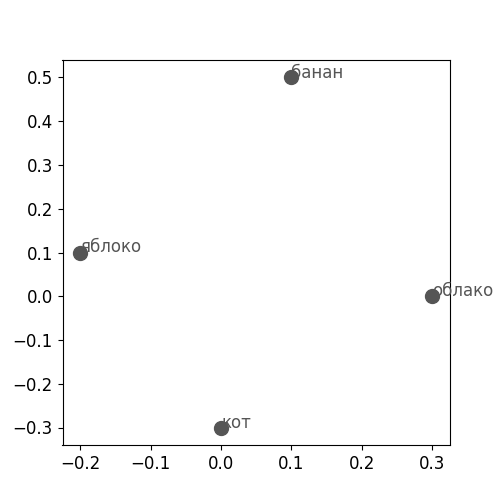
\includegraphics[width=0.4\textwidth]{img/alignment/alignment_1}}
    \hfill
    \subfloat[Эмбеддинги для слов из эпохи 2.\label{fig:alignment2}]
    {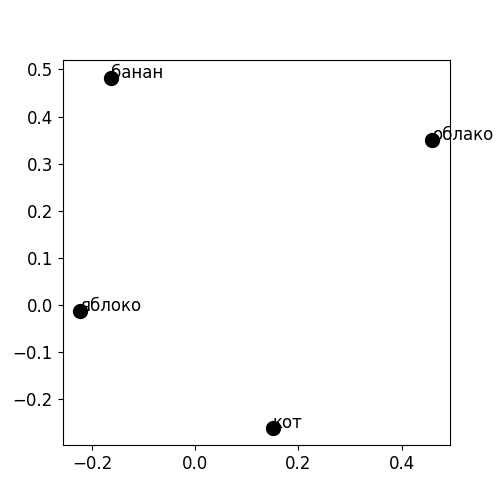
\includegraphics[width=0.4\textwidth]{img/alignment/alignment_2}}
    \\
    \subfloat[Эмбеддинги эпохи 2 после применения метода Прокруста.\label{fig:alignment3}]
    {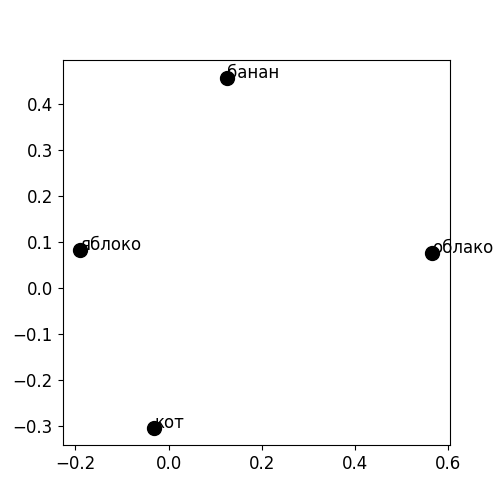
\includegraphics[width=0.4\textwidth]{img/alignment/alignment_3}}
    \hfill
    \subfloat[Сравнение векторных пространств. Выявление сдвига слова \textit{облако}.\label{fig:alignment4}]
    {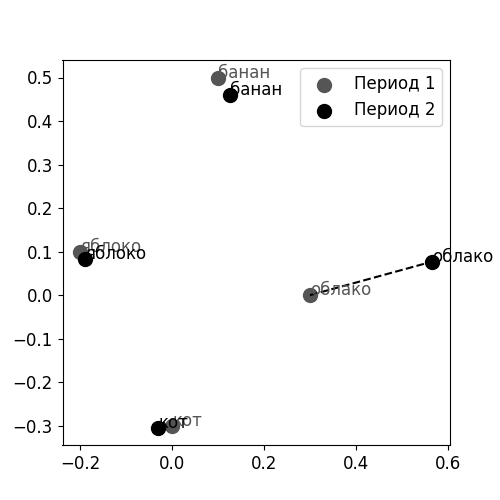
\includegraphics[width=0.4\textwidth]{img/alignment/alignment_4}}
    \caption{Пример поиска семантических изменений для статических эмбеддингов с использованием метода Прокруста.}
    \label{fig:mainfig_static_embeddings}
\end{figure}

Статические эмбеддинги оставались наиболее актуальными в задаче определения семантических изменений вплоть до 2020,
где показывали лучшие результаты в соревновании по обнаружению изменений значения слов SemEval-2020 Task 1~\cite{semeval2020task}.
%Они эффективно моделируют значение слов в зависимости от обучающего корпуса
%без опоры на объемные предобученные модели,
%превосходя по этому качеству модели, основанные на совстречаемости слов.

Среди недостатков статических эмбеддингов можно отметить:
\begin{itemize}
    \item необходимость большого объема слов в исследуемых корпусах для стабильности эмбеддингов,
    \item необходимость выравнивания моделей, обученных на отдельных наборах данных,
соответствующим временным срезам, что может вносить шум,
    \item моделируется только усреднённое значение слова на основе его употребления в корпусе,
не позволяя различать отдельные значения слова.
\end{itemize}

\subsection{Определение контекстуальных эмбеддингов}

Статические модели вложений слов присваивают каждому слову (лемме) один и тот же вектор
независимо от контекста, в то время как современные достижения в области обработки
естественного языка позволили разработать модели,
обеспечивающие получение контекстуализированных представлений высокого качества.
Данные модели присваивают токенам (минимальным единицам текста, с которыми работают модели,
обычно это слова, части слова или пунктуация) различные эмбеддинги
в зависимости от их контекста, что позволяет различать отдельные значения одного слова.

Например, в работе А.В. Кутузова приводится наглядный пример работы
контекстуальных эмбеддингов~\cite{Kutuzov2020Thesis}.
На Рисунке~\ref{fig:Контекстуальные вложения} показана проекция вложений ELMo для слова \textit{cell} (клетка)
в 2000-ые годы в английском языке.
На визуализации видны три кластера, отражающие различные значения слова \textit{cell} (клетка).
Два кластера, расположенные слева, представляют традиционные значения:
внизу биологическое значение, связанное с клетками живых организмов,
и вверху тюремное, где \textit{cell} означает камеру.
Кластер, который занимает правую сторону рисунка и чётко отделён от левых,
демонстрирует современное употребление слова \textit{cell},
где оно используется в контексте мобильной связи.

\begin{figure}[H]
	\centering
	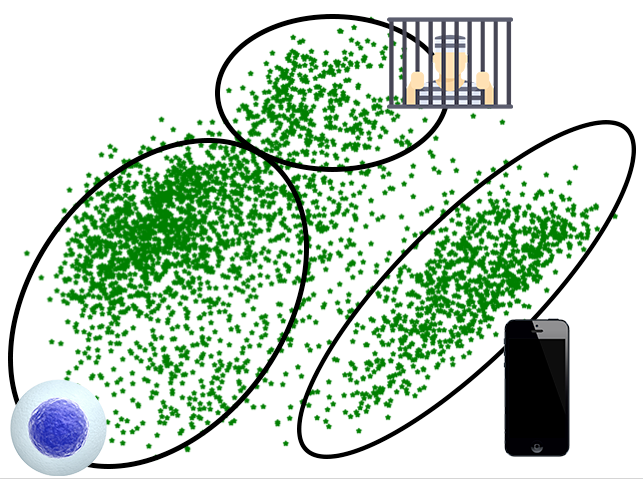
\includegraphics[width=0.75\textwidth]{img/theory/cell_projection_2000_photoshop}
	\caption{Проекция эмбеддингов использований слова \textit{cell} в 2000-ые годы}
	\label{fig:Контекстуальные вложения}
\end{figure}

Применение контекстуализированных векторных представлений задало новый стандарт для
высококачественных, чувствительных к контексту представлений в обработке естественного языка.
В работе, где исследователи использовали предварительно обученные модели BERT и ELMo,
%настроенные на полном корпусе Русского национального корпуса, было обнаружено,
настроенные на Национальном корпусе русского языка, было обнаружено,
что эти модели показывают значительную корреляцию с человеческими оценками
при определении диахронического семантического изменения слов в русском языке~\cite{rodina2020elmo}.
%Использовались алгоритмы, такие как косинусное сходство по прототипам слов и методы кластеризации,
%для выявления семантических сдвигов.

\subsection{Соревнование по выявлению семантических изменений Rushifteval}

Теме автоматического выявления семантических сдвигов для русского языка
было посвящено соревнование RuShiftEval, прошедшее в 2021 году~\cite{rushifteval}.
В ходе него участники должны были рассмотреть три исторических периода русского языка и общества:
предсоветский (1700-1916), советский (1918-1990) и постсоветский (1992-2016).
Исследование базировалось на наборе данных RuShiftEval, который состоит из
111 русских существительных (99 в тестовом наборе и 12 в наборе для разработки),
вручную аннотированных по степени изменения их значения в трех парах временных периодов.

Аннотаторам предлагалась задача, которую можно свести к оценке семантической связи между значениями
целевого слова в парах предложениях из разных временных периодов.
Оценки (от 1 до 4) отражают степень семантического сходства между значениями слова, где
1 обозначает отсутствие связи между значениями, а 4 – их совпадение.
Затем индивидуальные оценки усредняются, формируя общую меру семантического сходства между
употреблениями слова в разные временные периоды.
%Такая задача, как правило, называется Word-in-Context.

Вхождение в датасет Rushifteval представлено в Таблице~\ref{tab:Пример вхождения в датасет Rushifteval}.

\begin{table}[H]
\centering
\caption{Пример вхождения в датасет Rushifteval}
\label{tab:Пример вхождения в датасет Rushifteval}
\begin{tabular}{|>{\raggedright\arraybackslash}p{4cm}|>{\raggedright\arraybackslash}p{10cm}|}
\hline
\textbf{Слово} & радикал \\
\hline
\textbf{Предложение 1} & А вот социалисты и наши \textbf{\textit{радикалы}} – это совсем другого подбора. \\
\hline
\textbf{Предложение 2} & При некоторых условиях при отдельных элементарных реакциях возникают сразу два \textbf{\textit{радикала,}} что приводит к разветвлению цепи. \\
\hline
\textbf{Среднее} & 1.0 \\
\hline
\textbf{Аннотатор 1} & 1 \\
\hline
\textbf{Аннотатор 2} & 1 \\
\hline
\textbf{Аннотатор 3} & 1 \\
\hline
\end{tabular}
\end{table}

Для каждого из 99 целевых русских слов участники должны
были представить три значения, соответствующих семантическому изменению в упомянутых парах
временных периодов.
Эти значения использовались для построения трех ранжирований:
RuShiftEval-1 (изменение значений между досоветским и советским периодом),
RuShiftEval-2 (изменение значений между советским и постсоветским периодом)
и RuShiftEval-3 (изменение значений между досоветским и постсоветским периодом).
В качестве метрики оценки использовалась ранговая корреляция Спирмена между ранжированием слов,
сгенерированным системой, и эталонным ранжированием, полученным ручной аннотацией.
После этого бралась средняя оценка между ранжированиями.

Пример того, как выглядит эталонный файл с оценками, представлен в Таблице~\ref{tab:goldset_rushifteval}.

\begin{table}[H]
\centering
\caption{Отрывок тестового файла, содержащего обобщённые оценки аннотаторов}
\label{tab:goldset_rushifteval}
\begin{tabular}{|l|p{2.75cm}|p{2.75cm}|p{2.75cm}|}
\hline
\textbf{слово} & \textbf{досоветский: советский} & \textbf{советский: постсоветский} & \textbf{досоветский: постсоветский} \\
\hline
авторитет & 3.233 & 2.956 & 2.844 \\
\hline
амбиция & 3.111 & 3.444 & 3.333 \\
\hline
апостол & 3.494 & 3.427 & 3.424 \\
\hline
благодарность & 3.233 & 3.567 & 3.656 \\
\hline
\end{tabular}
\end{table}

Победители вышеупомянутого соревнования (команда GlossReader) указывают,
что проблемой в существующих решениях являлось то,
что эмбеддинги несут в основном информацию о форме слова, а не значении~\cite{GlossReader}.
Чтобы решить это, они дообучали модель XLM-R на задаче генерации эмбеддингов, максимально близким
к таким, какие получены на соответстующим использованиям слов словарным определениям
~\cite{XLM-R}.

При дообучении их система включает в себя два отдельных кодировщика на основе XLM-R:
Кодировщик контекcтов для кодирования использований целевых слов и
кодировщик определений для кодирования значения слова.
Система обучается, минимизируя расстояние между векторным представлением слова и соответствующим ему
определению.
При этом для обучения использовались данные только по английскому языку,
но модель также показала хорошие результаты для русского языка.

Далее, исследователи получали эмбеддинги пар контекстов слов с помощью
кодировщика контекстов, высчитывали расстояние между эмбеддингами с помощью различных метрик,
самым эффективным из которых были евклидово расстояние с нормализацией, после чего
логистическая регрессия приводила значения к формату датасета, то есть к значениям от 1 до 4.

%Авторы статьи предоставляют доступ к части исходного кода их исследования~\citeurl{GlossReaderGitHub}.
%Так, были опубликованы следующие компоненты:
%\begin{enumerate}
%    \item программный модуль генерации прогнозов на основе заранее вычисленных эмбеддингов,
%полученных с использованием обученной нейросетевой модели,
%    \item программный модуль оценки результатов.
%\end{enumerate}

%В то же время, авторы исследования не представили в открытый доступ следующие части:
%\begin{enumerate}
%    \item программный модуль предварительного обучения модели.
%    \item программный модуль для получения контекстуализированных
%    эмбеддингов, сформированных на основе предварительно обученной нейросетевой модели.
%\end{enumerate}

%Результаты исследования были нами воспроизведены и представлены в таблице~\ref{tab:GlossReader}.
%
%\begin{table}[H]
%\centering
%\caption{Коэффициэнты корреляции}
%\label{tab:GlossReader}
%\begin{tabular}{|l|c|}
%\hline
%Пары периодов                  & Коэффициент корреляции \\
%\hline
%Среднее            & 0.8021                  \\
%\hline
%досоветский:советский           & 0.7808                  \\
%\hline
%советский:постсоветский          & 0.8032                  \\
%\hline
%досоветский:постсоветский      & 0.8223                  \\
%\hline
%\end{tabular}
%\end{table}

Среди недостатков работы можно отметить неспособность модели корректно выявлять
значения тех слов, которые отличаются от ближайших аналогов в английском, например,
\textit{пионер}, связанный с коммунистической идеологией и не соответствующий в полной мере
слову \textit{scout}.

Второй подход к решению задачи определения семантических изменений был также получен
в рамках соревнования RuShiftEval и представлен в ~\cite{DeepMistake}.
%Кроме того, команда DeepMistake представила решение, занявшее в соревнование второе место
%~\cite{DeepMistake}.
%Однако, они смогли доработать его и повысить результаты до первого уже после окончания
%соревнования.

Исследователи обучали XLM-R на обширном многоязычном датасете с оценками аннотаторов,
затем дообучали ее на наборе данных RuSemShift (аналог Rushifteval с другими лексемами)
для настоящей задачи.
%В отношении архитектуры авторы утверждают, что применение линейного слоя на верхнем уровне,
%основанного на объединении L1-метрики и скалярного произведения между контекстуализированными
%эмбеддингами XLM-R, показывает лучшую производительность по сравнению с
%более традиционными подходами, такими как конкатенация эмбеддингов и
%использование нелинейных классификаторов.

%Исследователи выложили исходный код полностью и предлагают возможность воспроизвести их
%результат~\citeurl{DeepMistakeGitHub}.
%Результаты исследования были нами воспроизведены и представлены в таблице~\ref{tab:DeepMistake}.
%
%\begin{table}[H]
%\centering
%\caption{Коэффициэнты корреляции}
%\label{tab:DeepMistake}
%\begin{tabular}{|l|c|}
%\hline
%Пары периодов                  & Коэффициент корреляции \\
%\hline
%Среднее            & 0.8494                  \\
%\hline
%досоветский:советский           & 0.8563                  \\
%\hline
%советский:постсоветский          & 0.841                  \\
%\hline
%досоветский:постсоветский      & 0.8511                  \\
%\hline
%\end{tabular}
%\end{table}

Среди недостатков статьи можно выделить то, что авторы не предоставляют возможность визуализации
или интерпретации результатов, кроме непосредственно получившегося значения метрики.

Тем не менее, применимость таких методов была подвергнута сомнению в работе
\cite{DefinitionGenerationMainArticle},
где
%ставится под сомнение широкая практичность ранее упомянутых подходов. Они
утверждается, что такие методы практически неинтерпретируемы,
поскольку они не дают описаний значений слов,
а лишь бинарные результаты наличия или отсутствия семантического изменения.
Исследование, которое в наибольшей степени занимается этой проблемой, – это GlossReader~\cite{GlossReader},
где исследователи предлагают способ визуализации и интерпретации результатов.
Однако у этого метода есть свои недостатки, обсуждаемые выше, а также
необходимость определять заранее значения, для которых будет строиться визуализация.
Учитывая эти факты, новый подход моделирования определений,
является актуальным для задачи обнаружения семантических изменений.

\subsection{Моделирование определений}

Моделирование определений (также генерация определений) описывается исследователями как
«задача генерации определений слов в формате,
который может быть прочитан людьми, как те, что можно найти в словарях»,
где на вход подается целевое слово и пример его использования, а на выход
ожидается сгенерированное определение~\cite{DefinitionGenerationMainArticle}.
Пример представлен в Таблице~\ref{tab:Definition modeling example}.

\begin{table}[H]
\centering
\caption{Пример моделирования определений}
\label{tab:Definition modeling example}
\begin{tabular}{|l|p{8cm}|}
\hline
\textbf{Пример использования} & Примерно половина солдат в наших стрелковых взводах были призывниками, которых мы обучали около шести недель. \\
\hline
\textbf{Целевое слово} & призывник \\
\hline
\textbf{Сгенерированное определение} & Человек, который подлежит призыву в вооруженные силы \\
\hline
\end{tabular}
\end{table}

Начало интереса к моделированию определений как теме исследования
в области обработки естественного языка можно отнести
к исследованию~\cite{noraset2016definition}.
В работе они исследовали потенциал использования векторных представлений слов
для автоматической генерации определений.
Изначально была поставлена упрощенная задача с моносемантическими словами,
которые, имеют одно значение и, следовательно, одно определение.

Однако оставалась нерешенной проблема многозначных слов.
\cite{gadetsky-etal-2018-conditional} выделили важное условие для моделирования определений:
необходимость контекста для точного описания значений.
Было предложено включить примеры использований слова для предоставления контекста модели,
что оказалось решающим шагом в возможности модели справляться с полисемией и улучшении
ее производительности.

Несмотря на достижения, сделанные вышеупомянутыми исследователями,
область моделирования определений все еще сталкивалась с значительными проблемами.
Так, у данных подходов есть следующие недостатки~\cite{huang-etal-2021-definition}:
\begin{itemize}
    \item проблема слов вне словаря, когда модели сталкиваются с трудностями в работе со словами,
не встречавшимися во время обучения,
    \item проблемы избыточной и недостаточной специфичности в определениях.
\end{itemize}
Исследователи сообщают: «Избыточно специфичные определения представляют узкие значения слов,
в то время как недостаточно специфичные определения представляют общие и
нечувствительные к контексту значения.»
В \cite{huang-etal-2021-definition} предлагается использовать предварительно обученную модель энкодера-декодера,
а именно Text-to-Text Transfer Transformer (T5),
и ввели механизм ранжирования, предназначенный для тонкой настройки специфичности
генерируемых определений.
Метод был протестирован и продемонстрировал значительное
улучшение по сравнению с предыдущими решениями.

На момент написания работы, по мнению автора, лучший реализацией метода моделирования определений
является решение, представленное в \cite{DefinitionGenerationMainArticle}.

Авторы определяют задачу генерации определений следующим образом: для заданного слова \(w\) и примера
использования \(s\) (предложения, содержащего \(w\)) необходимо сгенерировать определение \(d\) на
естественном языке, которое будет грамматически корректным и точно передавать значение слова
\(w\) в контексте его использования.
Для генерации определений они используют модель Flan-T5, версию трансформера T5,
большую генеративную языковую модель,
дополнительно обученную на 1800 задачах по обработке естественного языка.

%Первым шагом исследователи выбирают, используя метрики BLEU, NIST, BERTScore, наиболее
%подходящий под задачу промпт из нескольких вариантов, например
%«what is the definition of <trg>?» или «define the word <trg>».

Для дообучения модели авторы используют три датасета, каждый из которых содержит определения
слов, сопровождаемые примерами употребления: WordNet, данные Оксфордского словаря и CoDWoE,
основанный на определениях и примерах, извлеченных из Викисловаря.

Для оценки качества модели исследователи предлагают использовать метрики SacreBLEU, ROUGE-L и BERT-F1.

Для демонстрации работы со сгенерированными определениями авторы
работы используют датасет, в котором слова представлены в графах диахронного использования
слов (Diachronic Word Usage Graphs, DWUG), взвешенных, ненаправленных графах,
узлами которых служат примеры использования слов, а веса рёбер отражают семантическую
близость пар употреблений.
DWUG созданы на основе многоэтапного процесса аннотации экспертами, в ходе которого аннотаторы
оценивали семантическое сходство пар употреблений слов по 4-балльной шкале
по схожей схеме с датасетом соревнования Rushifteval.

Прежде всего, авторы исследования проводят анализ корреляции между близостью пар слов в DWUG
и контекстуальными эмбеддингами токенов, эмбеддингами предложений примеров использования, а также
сгенерированными определениями и эмбеддингами, полученными на основе них.
Результаты показали, что сгенерированные определения обладают более высокой степенью
корреляции с данными из DWUG, чем контекстуальные эмбеддинги.

%Далее исследователи анализируют пространство эмбеддингов определений слов,
%чтобы выяснить, как они могут помочь в различении разных значений слов.
Кроме того, исследователи обнаружили, что эмбеддинги определений образуют более плотные и четко определенные
кластеры по сравнению с традиционными эмбеддингами, что делает их
подходящими для представления значений слов.

Далее авторы исследовали возможность присваивать кластерам, полученным на основе данных из DWUG,
соответствующие им определения.
Для обобщения определений в одном кластере авторы использовали самое прототипическое из них.
Они представляли все определения с помощью их эмбеддингов предложений и выбирали в качестве
прототипичного определение такое, эмбеддинг которого наиболее близок к среднему значению всех
эмбеддингов в кластере.

Авторы приходят к выводу, что сгенерированные определения слов могут играть роль
семантического представления слов, аналогичную традиционным эмбеддингам.
Они находят большие языковые модели достаточно развитыми для генерации определений
простым промптом.
При этом полученные таким образом определения превосходят по качеству
традиционные эмбеддинги и являются более наглядными.

\section{Метрики оценки качества сгенерированных определений}

При запуске модели на тестовой части датасета,
представляется возможным сравнить каждое полученное определение с эталонным определением из датасета.

Одним из основных способов оценки сгенерированных определений являются метрики
сходства строк~\cite{DefinitionModelingReviewAndDatasetAnalysis}.

Примером такой метрики является BLEU (Bilingual Evaluation Understudy).
BLEU — это стандартный алгоритм, используемый для оценки машинных переводов~\cite{BLUE}.
BLEU рассчитывается как точность n-грамм, то есть отношение правильных n-грамм к общему числу n-грамм в выходной строке.
Недостатком BLEU является то, что он оценивает только совпадение n-грамм.

\begin{equation}
\text{BLEU} = \exp \left( \text{BP} + \sum_{n=1}^{N} w_n \log p_n \right),
\end{equation}

где \(\text{BP}\) — это brevity penalty, который вычисляется как

\begin{equation}
\text{BP} = \min\left(1 - \frac{L_r}{L_c}, 0 \right),
\end{equation}

где \(L_r\) — длина эталонного определения,
\(L_c\) — длина сгенерированного определения,
\(w_n\) — веса для n-грамм,
\(p_n = \frac{\text{Число пересечений n-грамм}}{\text{Общее число n-грамм в сгенерированном тексте}}\) — точность n-грамм,.

Например, для текстов \textit{Кошка залезла на шкаф} и \textit{Кошка залезла на стол} BLEU будет равен 59.46 (от 100).

%Например, для текстов \textit{Кошка залезла на шкаф} и \textit{Кошка залезла на стол} будет рассчитываться так:
%
%Для простоты рассмотрим биграммы более подробно, а остальные параметры сразу укажем.
%
%\begin{enumerate}
%    \item Биграммы текста 1: \textit{Кошка залезла}, \textit{залезла на}, \textit{на шкаф}
%
%Биграммы текста 2: \textit{Кошка залезла}, \textit{залезла на}, \textit{на стол}
%    \item Считаем точность биграмм:
%
%Совпавшие биграммы: \textit{Кошка залезла}, \textit{залезла на}
%
%Точность биграмм (p2): 2/3
%    \item Штраф за краткость (BP):
%
%Длина эталонного текста (Lr): 4 слова
%
%Длина перевода (Lc): 4 слова
%
%BP = min(1, Lr / Lc) = min(1, 4/4) = 1
%    \item Итоговый расчет BLEU:
%
%Для униграмм (p1): 0.75
%
%Для триграмм (p3): 0.5
%
%Для четырехграмм (p4): 0.0
%    \item Подставляем значения (вместо логарифма 0.0 подставим 0.1, чтобы избежать деления на ноль):
%\[
%\text{BLEU} = 1 \cdot \exp \left( \frac{1}{4} (\log 0.75 + \log 0.6667 + \log 0.5 + \log 0.1) \right)
%\]
%\end{enumerate}

%Итак, BLEU score для \textit{Кошка залезла на шкаф} и \textit{Кошка залезла на стол} составляет примерно 59.46 (от 100).

Еще одной популярной метрикой является ROUGE-L (Recall-Oriented Understudy for Gisting Evaluation).
ROUGE измеряет совпадение n-грамм между эталонным и кандидатом на определение~\cite{ROUGE}.
ROUGE-L — это модифицированная версия ROUGE, которая использует наибольшую общую подпоследовательность
для измерения сходства между двумя определениями.
Преимуществом ROUGE-L является то, что он автоматически определяет самые длинные последовательные общие n-граммы.
Формула для расчета ROUGE-L выглядит следующим образом:

\begin{equation}
\text{ROUGE-L} = \frac{LCS(X, Y)}{L_r}
\end{equation}

где $LCS(X, Y)$ — длина наибольшей общей подпоследовательности между строками $X$ и $Y$, а $L_r$ — длина эталонного определения.

Например, для \textit{Кошка залезла на шкаф} и \textit{Кошка залезла на стол} ROUGE-L составит 0.75 (от 1).

Тем не менее, у таких метрик есть недостаток.
Они анализируют не семантику слов, а только буквальное совпадение n-грамм между ними.

Примером более продвинутой метрики является BERTScore.
BERTScore (Bidirectional Encoder Representations from Transformers) — это метрика,
которая вычисляет оценку сходства между кандидатом и эталонным определением
на основе предварительно обученных контекстуальных эмбеддингов из BERT~\cite{BERTScore}.
BERTScore вычисляет точность~\eqref{eq:Precision}, полноту~\eqref{eq:Recall} и F1-меру~\eqref{eq:F1}.
Формулы для расчета BERTScore выглядят следующим образом:

\begin{equation}
\text{Precision} = \frac{1}{|C|} \sum_{x \in C} \max_{y \in R} \text{cos}(x, y)\label{eq:Precision}
\end{equation}

\begin{equation}
\text{Recall} = \frac{1}{|R|} \sum_{y \in R} \max_{x \in C} \text{cos}(x, y)\label{eq:Recall}
\end{equation}

\begin{equation}
\text{F1} = 2 \cdot \frac{\text{Precision} \cdot \text{Recall}}{\text{Precision} + \text{Recall}}\label{eq:F1}
\end{equation}

где $C$ — множество токенов кандидата, $R$ — множество токенов эталона,
и $\text{cos}(x, y)$ — косинусное сходство между эмбеддингами токенов $x$ и $y$.

Например, для текстов \textit{выложил документ в удалённое хранилище}, \textit{выгрузил файл в облако}
значение BERT-F1 – 76.21 (от 100), несмотря на непосредственное совпадение лишь одного слова.

Использование нескольких метрик позволяет получить более полную картину качества модели,
поскольку каждая из них оценивает разные аспекты сгенерированного текста.
Как традиционные BLEU и ROUGE-L, так и более современный BERT-F1 активно используются в
задачах обработки естественного языка, в том числе в задачах генерации текста~\cite{BLUE,ROUGE,BERTScore}.
Так, в обзорной статье по моделированию определений утверждается, что на момент выпуска статьи метрика BLUE
использовалась в 9 научных публикациях по теме, а ROUGE-L и BERTScore – в 3~\cite{DefinitionModelingReviewAndDatasetAnalysis}.

\section{Классификация ошибок сгенерированных определений}

В работах \cite{huang-etal-2021-definition} и \cite{noraset2016definition} проводится оценка выборки сгенерированных определений,
для которой они предсталяют классификацию ошибок,
часто встречаемых в сгенерированных определениях.
Далее представлена классификация ошибок на основе классификации \cite{huang-etal-2021-definition}.

Исключением является «Избыточность или чрезмерное использование общих фраз»,
которую авторы опустили в исследовании из-за её редкости.
%Данный тип ошибки будет описан нами.

Таким образом, ошибками являются:

\begin{enumerate}
\item \textbf{Избыточное конкретизирование.} Определение даёт слишком узкое описание слова.

   Слово: дуновение

   Пример: дуновение – ’движение неприятного запаха через воздух’.

   Эталонное определение: «Лёгкий порыв ветра; движение воздуха.»~\cite{TolkovyKuznetsov}

   Объяснение ошибки: Ошибка заключается в том, что определение ограничивает значение слова компонентом ’неприятный запах’, тогда как оно имеет более широкое значение.

\item \textbf{Недостаточное конкретизирование.} Определение даёт слишком общее или неполное описание.

   Слово: капитан

   Пример: капитан – ’член команды’.

   Эталонное определение: «Командир, начальник судна.»~\cite{TolkovyKuznetsov}.

   Объяснение ошибки: Ошибка заключается в отсутствии указания на ключевые семантические компоненты руководящей роли капитана, что приводит к недостаточной конкретизации значения слова.

\item \textbf{Самореференция.} Определение содержит само слово или его производные.

   Слово: самосознание

   Пример: самосознание – ’состояние, при котором у человека присутствует самосознание’.

   Эталонное определение: «Полное понимание самого себя, своего значения, роли в жизни, обществе.»~\cite{TolkovyKuznetsov}.

   Объяснение ошибки: Ошибка заключается в том, что в определении не раскрывается семантическая сущность слова, так как для описания значения используется само же рассматриваемое слово.

\item \textbf{Неправильная часть речи.} Модель даёт такое определение, которое относится к лексеме другой части речи.

   Слово: стекло

   Пример: стекло – ’переместиться вниз, сбежать (о жидкости)’ для контекста «После урока стекло оказалось сломанным.»

   Эталонное определение: «изделие из твёрдого прозрачного материала.»~\cite{TolkovyDmitriev}

   Объяснение ошибки: Определение относится к глаголу \textit{стекло}, тогда как слово в контексте является существительным.

\item \textbf{Противоположное значение.} Определение выражает смысл, противоположный истинному значению слова.

   Слово: внутрь

   Пример: внутрь – ’ненаправленный в центр’.

   Эталонное определение: «Во внутреннюю часть, в пределы, в глубину, в середину.»~\cite{TolkovyKuznetsov}.

   Объяснение ошибки: Определение выражает противоположное значение истинному значению слова.

\item \textbf{Близкая семантика.} Определение верно передает только часть компонентов значения.

   Слово: машина

   Пример: машина – ’устройство с автоматическими функциями’.

   Эталонное определение: «Механизм или совокупность механизмов, совершающие какую-л. полезную работу путём преобразования одного вида энергии в другой.»~\cite{TolkovyKuznetsov}.

   Объяснение ошибки: Определение верно передает только основную сему \textit{’механизм’}, предлагая совершенно необязательную сему \textit{’автоматизированности’} и упуская семы совершения полезной работы.

%   Слово: милый
%
%   Пример 2: милый – ’имеющий признаки ребёнка’.
%
%   Эталонное определение: Затычка.
%
%   Объяснение ошибки: Определение не охватывает все значения, связанные с этим словом.

\item \textbf{Некорректность.} Определение полностью ошибочно и не соответствует значению слова.

   Слово: первый

   Пример: первый – ’следующий после всех остальных в списке предметов’.

   Эталонное определение: «При счёте вы называете первым предмет, элемент, человека и т. д., с которого начинаете счёт.»~\cite{TolkovyDmitriev}

   Объяснение ошибки: Определение полностью ошибочно.

%   Слово: упаковать
%
%   Пример 2: упаковать – ’сделать внезапный звук’.
%
%   Эталонное определение: Затычка.
%
%   Объяснение ошибки: Определение полностью ошибочно.

\item \textbf{Избыточность или чрезмерное использование общих фраз.} Определение содержит повторы или избыточные формулировки.

%   Слово: пропан
%
%   Пример 1: пропан – ’горючий газ, используемый для горения газа’.
%
%   Эталонное определение: Затычка.
%
%   Объяснение ошибки: Определение содержит избыточные формулировки.

   Слово: спутник

   Пример: спутник – ’тот, кто совершает путь, путь вместе с кем-л.’.

   Эталонное определение: «Тот, кто совершает путь вместе с кем-л.»~\cite{TolkovyKuznetsov}.

   Объяснение ошибки: Определение содержит повтор слова \textit{путь}.

\end{enumerate}

Также среди определений можно выделить:
\begin{itemize}
\item \textbf{Корректные.} Определение точно и в нужной степени полно передает значение слова и не содержит какие-либо из вышеописанных ошибок.

   Слово: винодельня

   Пример: винодельня – ’заведение, помещение для изготовления вина’.

   Эталонное определение: «Заведение, место, где изготовляется виноградное вино.»~\cite{ushakov1940}

   Объяснение: Определение точно и полно передает значение слова.
\end{itemize}

\section*{Выводы}

В последние годы возрос интерес к полуавтоматическим
и автоматическим подходам выявления семантических изменений,
основанным на векторных представлениях слов (эмбеддингах).
Статические эмбеддинги, обучаемые на корпусах текстов, позволяют выявлять семантические сдвиги,
однако имеют ограничения, связанные с необходимостью выравнивания моделей и неразличением значений
отдельного слова.
Контекстуальные эмбеддинги, генерируемые современными языковыми моделями,
показывают более высокую точность в задачах обнаружения семантических изменений,
поскольку учитывают контекст употребления слов.

Новым перспективным направлением является использование моделирования определений слов
на основе генеративных больших языковых моделей.
Сгенерированные определения демонстрируют более высокую корреляцию с данными о семантической близости слов,
чем традиционные эмбеддинги, и могут служить семантическим представлением слов,
превосходящим по качеству векторные репрезентации.
Существует несколько способов оценки сгенерированных определений:
от метрик сходства текста до классификаций для качественного анализа.

Тем не менее, моделирование определений остаётся недостаточно исследованной темой
в контексте семантических изменений, особенно на материале русского языка.

\chapter{Предлагаемый подход}

%Методология настоящей работы заключается в следующем.

В данном исследовании предлагается метод моделирования определений слов,
который характеризуется как задача генерации определений в формате,
доступном для чтения людьми, аналогично тем, что представлены в словарях.
Входными данными для модели служат целевое слово \( w \) и пример его использования в предложении \( s \),
на выходе генерируется определение \( d \).

Основными этапами предлагаемого подхода являются:

\textbf{Этап 1}: Обучение

Пусть имеется датасет \( D = \{(w_i, s_i, d_i)\}_{i=1}^{N} \),
где \( w_i \) — это слово, \( s_i \) — пример его использования в предложении,
а \( d_i \) — определение данного слова.
Целью первого этапа является обучение генеративной большой языковой модели.
Модель \( M \) обучается на данных словаря, содержащих определения слов и их контекст использования,
с целью генерации определений слов, аналогичных тем, что можно найти в словарях.
Формально, модель \( M \) обучается минимизировать функцию потерь \( L \), определенную как:

\begin{equation}
L(M) = \sum_{i=1}^{N} \text{loss}(M(w_i, s_i), d_i),
\end{equation}

где \(\text{loss}\) — это функция потерь,
измеряющая расхождение между сгенерированным определением и эталонным определением.

\textbf{Этап 2}: Тестирование

На втором этапе проводится тестирование обученной модели по ряду метрик.
Этот этап включает:

1. Генерацию определений для тестовой выборки \( D_{\text{test}} = \{(w_j, s_j, d_j)\}_{j=1}^{P} \)
и последующую оценку качества сгенерированных определений \( \hat{d}_j = M(w_j, s_j) \) относительно
эталонных определений \( d_j \).
Для оценки качества используются меры сходства текста, которые оценивают формальную схожесть или семантику сравниваемых текстов.
Формально, метрика \( \text{metric} \) определяется как:

\begin{equation}
\text{metric} = \frac{1}{M} \sum_{j=1}^{P} \text{similarity}(\hat{d}_j, d_j)
\end{equation}

где \(\text{similarity}\) — такая функция, измеряющая сходство между сгенерированным и эталонным определениями,
как BLEU, ROGUE-L и BERT-F1.

2. Проверку модели на датасете, посвященном детектированию семантических изменений и
содержащих оценки аннотаторов между парами вхождений.

Для каждой пары использований слов в датасете генерируются определения \( (\hat{d}_{k1}, \hat{d}_{k2}) \),
которые затем векторизуются \( (\vec{d}_{k1}, \vec{d}_{k2}) \).
Полученное значение расстояния между векторизованными определениями \( \text{dist}(\vec{d}_{k1}, \vec{d}_{k2}) \)
сравнивается с оценками аннотаторов в датасете.

\textbf{Этап 3}: Визуализация

Для визуализации семантических изменений слов полученные с помощью модели определения векторизуются
с помощью векторизатора \( V \).
   \begin{equation}
   \mathbf{v}_i = V(d_i)
   \end{equation}

Определения, имеющие семантически близкие значения,
группируются с использованием алгоритма кластеризации \( C \).
   \begin{equation}
   \{K_1, K_2, \ldots, K_m\} = C(\{\mathbf{v}_1, \mathbf{v}_2, \ldots, \mathbf{v}_n\})\text{,}
   \end{equation}
   где \( m \) – количество кластеров.

Для каждого кластера \( K_j \) выбирается прототипическое определение \( \hat{d}_{\text{proto}} \),
которое определяется как наиболее близкое к центру кластера (центроиду).

Пусть \( \mathbf{c}_j \) — центроид кластера \( K_j \):

\begin{equation}
\hat{d}_{\text{proto}, j} = \arg\min_{\mathbf{v} \in K_j} d(\mathbf{v}, \mathbf{c}_j)\text{,}
\end{equation}

где \( d \) — метрика расстояния.

Затем создаются столбчатые диаграммы,
отражающие частоту употреблений различных значений слова во времени,
с обозначением категорий цветовой градацией и легендой.

\textbf{Этап 4}: Качественный анализ

Проводится качественный анализ результатов, полученных с помощью визуализаций,
на наборе слов из \cite{TwoCenturies}.
Полученные определения сравниваются с информацией из семантических описаний слов,
написанных на основе метода обобщения словарных дефиниций И.А. Стернина~\cite{SemanticDefinitionsAndAnalysis},
и классифицируются на основе классификации ошибок,
сделанной на основе \cite{huang-etal-2021-definition},
а статистическая информация о частоте использования тех или иных значений сравнивается
с информацией из \cite{TwoCenturies}.

%Настоящее исследование базируется на методе моделирования определений,
%который определяется исследователями как «задача генерации определений слов в формате,
%который может быть прочитан людьми, как те, что можно найти в словарях»,
%где на вход подается целевое слово, пример его использования, а на выход
%ожидается сгенерированное определение.
%
%На первом этапе исследования планируется обучение генеративной языковой модели
%на основе архитектуры Трансформер.
%Данная модель будет обучена на данных словаря,
%содержащих определения слов и их контекст использования, с целью генерации определений слов,
%аналогичных тем, что можно найти в словарях.
%
%На втором этапе работы планируется провести тестирование обученной модели на метриках.
%Этот этап включает в себя, во-первых, генерацию определений для тестовой выборки
%и последующую оценку качества сгенерированных определений относительно
%эталонных определений из тестовой выборки для оценки точности и качества работы модели.
%Для оценки качества будут использоваться меры сходства текста,
%которые оценивают формальную схожесть или семантику сравниваемых текстов.
%Во-вторых, этот этап включает проверку модели на датасете соревнования Rushifteval,
%посвященному детектированию семантических изменений.
%Для каждой пары использований слов в датасете будут сгенерированы определения,
%которые позже будут векторизованы.
%Далее будет получено значение, насколько расстояние между векторизованными определениями
%совпадает с оценками аннотаторов в датасете.
%
%После тестирования модели на третьем этапе будет осуществляться визуализация
%результатов работы модели столбчатыми графиками.
%
%Также будет проведен качественный анализ результатов, полученных с помощью визуализаций,
%на наборе из слов.
%Полученные определения будут сравниваться с таковыми из словарей,
%а статистическая информация о частоте использования тех или иных значений
%будет сравниваться с информацией из лексикографических изданий.
%
%Действия, описанные далее, подкрепляются кодом, выложенным в открытый доступ, на сайте GitHub
%и могут быть воспроизведены.~\cite{WorkGitHub}

\chapter{Анализ предлагаемого подхода}

\section{Обучение языковой модели на данных тезауруса}

В качестве модели была выбрана FRED-T5-1.7B, являющаяся одной из новейших языковых моделей,
выпущенных SberDevices и обученных с нуля на материале русского языка~\cite{FRED-T5}.
Для выбора модели использовался бенчмарк для оценки продвинутого понимания русского языка
RussianSuperGLUE~\cite{RussianSuperGLUE}.
В бенчмарке присутствуют несколько групп задач, охватывая
общую диагностику языковых моделей и различные лингвистические задачи:
понимание здравого смысла, логическое следование в естественном языке,
рассуждения, машинное чтение и знания о мире.
На момент написания работы FRED-T5-1.7B занимает самое высокое место в лидерборде данного бенчмарка,
со значением 0.762,
уступая лишь результатам выполнения данных заданий людьми со значением 0.811,
что свидетельствует о ее способности к выдающемуся языковому пониманию и анализу.
Таким образом, FRED-T5-1.7B представляется наиболее подходящей языковой моделью
для задачи генерации определений.

Одной из ключевых особенностей модели FRED-T5-1.7B является наличие денойзеров.
Денойзеры — это специальные механизмы, задача которых состоит в очистке текста от шума,
то есть в восстановлении удаляемых или искажаемых частей текста.
В модели используется семь различных денойзеров, каждый из которых выполняет
уникальную функцию в процессе обучения.
Основные задачи денойзеров включают в себя:
\begin{itemize}
    \item восстановление удаленных участков текста;
    \item продолжение текстовых последовательностей.
\end{itemize}

Каждый из денойзеров помечен специальным токеном.
В настоящей работе при работе с моделью используется денойзер,
помеченный специальным токеном «<LM>»,
который задействован в задаче продолжения текста.

В качестве материала, используемого для обучения модели, выступил датасет,
включающий в себя материал из МАС – «Малого академического словаря»~\cite{MAS1981}.
Материал МАС был получен с помощью скраппера, написанного на языке Python.
В загруженном наборе данных в каждом вхождении присутствовали
идентификатор статьи, лексема, про которую написана данная статья, а также определения
с примерами использования.
Пример вхождения в набор данных представлен в Таблице~\ref{tab:Пример МАС}.
Определения выделены жирным.

\begin{table}[H]
\centering
\caption{Информация о лексеме из МАС} \\
\label{tab:Пример МАС}
\begin{tabular}{|m{4.5cm}|m{9.5cm}|}
\hline
\textbf{Лексема} & \textbf{Определения и примеры использования} \\
\hline
производительность & \textbf{Способность производить, выпускать то или иное количество продукции:} Производительность машин. Годовая производительность завода.
\newline \textbf{Целесообразность, плодотворность:} Производительность затрат. \\
\hline
\end{tabular}
\end{table}

Полученный материал был очищен от помет, вхождений, не имеющих при себе примеров использования,
или информативных определений, например, \textit{Состояние по знач. глаг. линять},
или не содержащих определений вовсе, а также имеющие такие определения,
которые несут грамматическую информацию о слове вместо лексического значения,
например, \textit{наречие к причастию приглашающий}.
В результате, было получено 122 тысяч 350 вхождений.

Примеры и слова были отформатированы под формат запроса модели.
В начале после слова «Контекст» шел пример использования слова, после чего шла фраза
«Определение слова», в которую включалось само слово.
Таким образом, на вход модель
принимает лексему и контекст, в которой она употреблялась, а на выход ожидается сгенерированное
определение.

\begin{table}[H]
\centering
\caption{Пример отформатированного запроса модели}
\begin{tabular}{|m{2.5cm}|m{9.5cm}|}
\hline
\textbf{Поле}       & \textbf{Значение}                                                                                          \\
\hline
input\_text  & <LM>Контекст: \("\)Усталость возьмет свое, тогда можно жестоко прозябнуть и опасно заболеть.\("\) Определение слова \("\)прозябнуть\("\): \\
\hline
\end{tabular}
\end{table}

FRED-T5-1.7B была дообучена на полученном из «Малого академического словаря» материале
в течение 6 эпох с линейным шагом обучения 0.001,
размером батча 16 и оптимизатором Adafactor на машине с одной видеокартой RTX 3090
с объёмом видеопамяти 24ГБ.
Обучение заняло 11 часов 10 минут. % TODO: вставить позже
Максимальное использование видеопамяти не превышало 11ГБ. % TODO: вставить позже
Для ускорения обучения и экономии видеопамяти использовалась технология LoRA со
следующими параметрами: r – 32, alpha
 – 64, dropout – 0.1, что позволило
уменьшить количество обучаемых параметров до 14155776 (0.8\% от общего числа параметров),
сэкономить используемую память и ускорить обучение.
В качестве метрики потерь (лосса) используется кросс-энтропия.
График потерь представлен на Рисунке~\ref{fig:loss-plot-epoch}.

\begin{FIGURE}[h]{Потери при обучении модели \label{fig:loss-plot-epoch}}
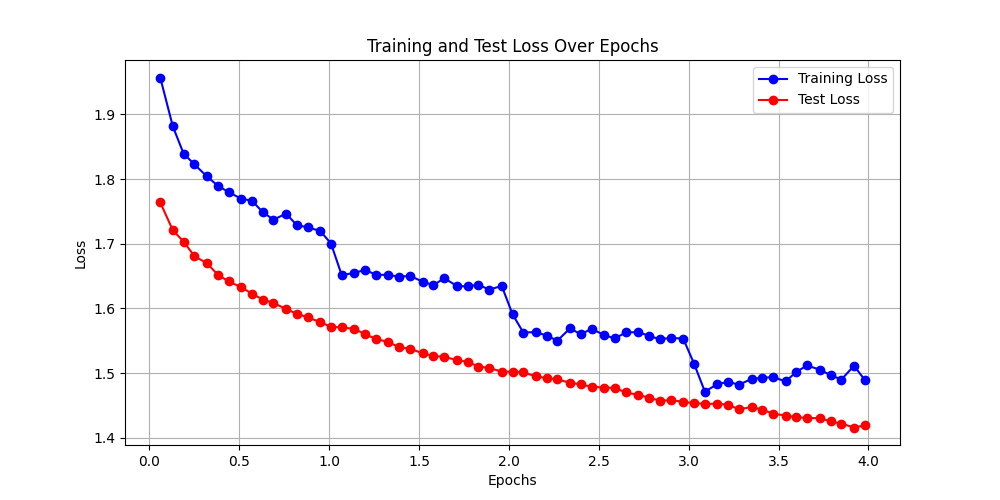
\includegraphics[width=0.8\textwidth]{img/loss-plot-epoch}
\end{FIGURE}

Более подробный обзор гиперпараметров модели доступен в Приложении Б.

\section{Тестирование модели метриками сходства строк}

%Для оценки качества обучения модели использовались метрики BLEU и ROUGE-L,
%которые оценивают формальную схожесть текста: BLEU оценивает точность совпадений n-грамм
%в сгенерированном тексте по сравнению с эталонным текстом~\cite{BLUE}, а ROUGE-L измеряет схожесть между
%сгенерированным текстом и эталонным текстом на основе наибольшей общей последовательности слов~\cite{ROUGE}.
%Также использовалась метрика BERT-F1, учитывающая семантику сравниваемых текстов благодаря
%использованию контекстуальных эмбеддингов при подсчете значения метрики~\cite{BERTScore}.
%Использование нескольких метрик позволяет получить более полную картину качества модели,
%поскольку каждая из них оценивает разные аспекты сгенерированного текста.
%Как традиционные BLEU и ROUGE-L, так и более современный BERT-F1 активно используются в
%задачах обработки естественного языка, в том числе в задачах генерации текста~\cite{BLUE,ROUGE,BERTScore}.
%Так, в обзорной статье по моделированию определений утверждается, что на момент выпуска статьи метрика BLUE
%использовалась в 9 научных публикациях, ROUGE-L и BERTScore – в 3~\cite{DefinitionModelingReviewAndDatasetAnalysis}.
%В настоящей работе результаты данных метрик будут сравниваться с таковыми из статьи
%Giulianelli M. et al., где сообщаются результаты трёх вышеперечисленных метрик при обучении модели
%Т5 для задаче генерации определений на английском языке~\cite{DefinitionGenerationMainArticle}.

В данной работе использовались версии метрик BLEU, ROUGE-L и BERT-F1, взятые из библиотеки \textit{evaluate}~\citeurl{Evaluate}.
Результаты оценки дообученной модели представлены в Таблице~\ref{tab:Similarity metrics}.

\begin{table}[H]
\centering
\caption{Результаты дообучения FRED-T5-1.7B на датасете МАС (от 100, больше – лучше)}
\label{tab:Similarity metrics}
\begin{tabular}{|l|c|}
\hline
Метрика                  & Значение \\
\hline
BLEU            & 11.02                  \\
\hline
ROUGE-L           & 29.36                  \\
\hline
BERT-F1          & 75.22                  \\
\hline
\end{tabular}
\end{table}

Тестирование показывает низкие значения метрик BLEU и ROUGE-L,
что говорит о том, что модель формулирует определения не так,
как они написаны в тестовой выборке.
Тем не менее, это не означает некорректность генерируемых определений.
Судя по результатам метрики BERT-F1, можно сказать, что семантически сгенерированные определения
совпадают с таковыми из тестовой выборки.
Такие результаты можно объяснить тем, что модель выдаёт семантически верные,
но иначе сформулированные определения.
Например, для слова \textit{отощалый} в контексте
«Иван Бедный сидел в развалившейся лачуге, худой, отощалый.»
ожидаемым определением являлось ’ставший тощим, отощавший’,
но моделью было сгенерировано ’сильно исхудавший от недоедания’.
Оба данных определения корректны и описывают того, кто стал худым,
но при этом между ними не совпадает ни единого токена.
Метрики BLEU и ROUGE-L для такой пары показывают 0.
Только BERT-F1 возвращает 70.39,
поскольку данная метрика вместо совпадения последовательности сравниваемых определений
использует векторизатор и сравнивает расстояние между полученными эмбеддингами,
которое обозначает семантическую близость двух текстов.

Следует сказать, что предварительный анализ полученных определений показал
наличие определений, имеющих ошибку самореференции.
Например, для контекста \textit{[Пантелей Прокофьевич] ничего не мог сделать, чтобы восстановить в семье прежний порядок.}
и целевого слова \textit{восстановить}
изначально было сгенерировано «привести в прежнее состояние; восстановить»,
что содержит повторение целевого слова,
а результаты метрик были ниже представленного ранее: 10.64 для BLEU, 29.09 для ROUGE-L, и 75.19 для BERT-F1.

Удалось значительно сократить количество определений с самореференцией,
исключив из генерации токены, соответствующие целевому слову.
Для этого мы заранее определяли все возможные формы целевого слова и
исключали их из процесса генерации определения,
что помогло избавиться от подобных ошибок и улучшить результаты.

%Мы смогли значительно снизить число определений,
%страдающих от проблемы самореференции добавлением в исключения токенов,
%используемых для кодирования целевого слова.
%
%Так, перед генерацией определения для каждого примера создаётся набор возможных
%вариантов написания целевого слова с помощью модуля \textit{pymorphy3},
%после чего кодируем используемым для инференса токенизатором и добавляем
%получившиеся токены в аргумент \textit{bad\_words\_ids} метода \textit{generate},
%что позволило избавиться от такого рода ошибок и повысило результаты.
Например, для контекста \textit{[Пантелей Прокофьевич] ничего не мог сделать, чтобы восстановить в семье прежний порядок.}
и целевого слова \textit{восстановить} после правки было сгененировано
«привести в прежнее состояние, положение».

\section{Тестирование модели на материале соревнования Rushifteval}

С помощью дообученной модели FRED-T5-1.7B были получены определения для тестовой части датасета
соревнования Rushifteval.

Для векторизации сгенерированных определений использовалась модель paraphrase-multilingual-mpnet-base-v2~\citeurl{Vectorizer}.
Данная модель является одним из лидеров по задаче семантической схожести текстов~\citeurl{Encodechka}.
Далее векторы были нормализированы, после чего расстояние между
векторным представлением определений считалось с помощью косинусного расстояния.
Результат приводился в формат значений датасета с помощью линейной регрессии,
тренированной на датасете Rusemeval.
Так, значения косинусного расстояния от 0 до 2, где 0 обозначает идентичность векторов,
а 2 – их противоположность, преобразованы в значения от 1 до 4,
соответствующие оценкам аннотаторов, где 1 – противоположные значения, а 4 – идентичные.
Результаты представлены в Таблице~\ref{tab:Rushifteval results default}.

\begin{table}[H]
\centering
\caption{Коэффициэнты корреляции с использованием LinReg}
\label{tab:Rushifteval results default}
\begin{tabular}{|l|c|}
\hline
\textbf{Пары периодов}                  & \textbf{Коэффициент корреляции} \\
\hline
Среднее            & 0.7156                  \\
\hline
досоветский:советский           & 0.7056                  \\
\hline
советский:постсоветский          & 0.7251                  \\
\hline
досоветский:постсоветский      & 0.7160                  \\
\hline
\end{tabular}
\end{table}

В качестве попытки улучшить результаты в течение трёх эпох
был дообучен векторизатор paraphrase-multilingual-mpnet-base-v2
на материале RuSemShift (аналог RuShiftEval с другими лексемами).
Результаты представлены в Таблице~\ref{tab:Rushifteval 2}.
Авторами соревнования рекомендуется дообучать решения на данном наборе данных для улучшения результатов.
Параметры дообучения векторизатора доступны в Приложении В.

\begin{table}[H]
\centering
\caption{Коэффициэнты корреляции с использованием LinReg и дообученного векторизатора}
\label{tab:Rushifteval 2}
\begin{tabular}{|l|c|}
\hline
\textbf{Пары периодов}                  & \textbf{Коэффициент корреляции} \\
\hline
Среднее            & 0.8002                  \\
\hline
досоветский:советский           & 0.7843                  \\
\hline
советский:постсоветский          & 0.8139                  \\
\hline
досоветский:постсоветский      & 0.8023                  \\
\hline
\end{tabular}
\end{table}

Таким образом, благодаря дообучению векторизатора была улучшена производительность алгоритма
на более чем 8\%.

\section{Сравнение с существующими подходами}

Рассмотрим полученные результаты в сравнении с аналогами из соревнования Rushifteval.

Исходный код лидирующих решений выложен в открытый доступ и доступен для воспроизводства.

Авторы статьи~\cite{GlossReader} предоставляют доступ к части исходного кода
их исследования~\citeurl{GlossReaderGitHub}.
Так, были опубликованы следующие компоненты:
\begin{enumerate}
    \item программный модуль генерации прогнозов на основе заранее вычисленных эмбеддингов,
полученных с использованием обученной нейросетевой модели,
    \item программный модуль оценки результатов.
\end{enumerate}

Результаты исследования были воспроизведены и представлены в Таблице~\ref{tab:GlossReader}.

\begin{table}[H]
\centering
\caption{Коэффициэнты корреляции}
\label{tab:GlossReader}
\begin{tabular}{|l|c|}
\hline
Пары периодов                  & Коэффициент корреляции \\
\hline
Среднее            & 0.8021                  \\
\hline
досоветский:советский           & 0.7808                  \\
\hline
советский:постсоветский          & 0.8032                  \\
\hline
досоветский:постсоветский      & 0.8223                  \\
\hline
\end{tabular}
\end{table}

Другой командой, представившей решение в открытый доступ является~\cite{DeepMistake}.

В Таблице~\ref{tab:DeepMistake} представлен воспроизведённый нами результат~\citeurl{DeepMistakeGitHub}.

%Исследователи выложили исходный код полностью и предлагают возможность воспроизвести их
%результат~\citeurl{DeepMistakeGitHub}.
%Результаты исследования были нами воспроизведены и представлены в таблице~\ref{tab:DeepMistake}.

\begin{table}[H]
\centering
\caption{Коэффициэнты корреляции}
\label{tab:DeepMistake}
\begin{tabular}{|l|c|}
\hline
Пары периодов                  & Коэффициент корреляции \\
\hline
Среднее            & 0.8494                  \\
\hline
досоветский:советский           & 0.8563                  \\
\hline
советский:постсоветский          & 0.841                  \\
\hline
досоветский:постсоветский      & 0.8511                  \\
\hline
\end{tabular}
\end{table}

%\begin{table}[H]
%\centering
%\caption{Результаты алгоритма в сравнении с результатами команд Rushifteval.}
%\begin{tabular}{|m{2.5cm}|m{3cm}|m{3cm}|m{3cm}|m{2.0cm}|}%m{1.5cm}|}
%\hline
%\textbf{Команда} & \textbf{досоветский:
%советский} & \textbf{советский:
%постсоветский} & \textbf{досоветский:
%постсоветский} & \textbf{Среднее} \\% & \textbf{Тип} \\
%\hline
%\textbf{DeepMistake (после соревнования)} & \textbf{0.863} & \textbf{0.854} & \textbf{0.834} & \textbf{0.850} \\% & token \\
%\hline
%GlossReader & 0.781 & 0.803 & 0.822 & 0.802 \\% & token \\
%\hline
%\textbf{FRED-T5-FN с дообучением векторизатора} & \textbf{0.784} & \textbf{0.814} & \textbf{0.802} & \textbf{0.800} \\% & \textbf{token} \\
%\hline
%DeepMistake & 0.798 & 0.773 & 0.803 & 0.791 \\% & token \\
%\hline
%vanyatko & 0.678 & 0.746 & 0.737 & 0.720 \\% & token \\
%\hline
%\textbf{FRED-T5-FN} & \textbf{0.706} & \textbf{0.725} & \textbf{0.716} & \textbf{0.716} \\% & \textbf{token} \\
%\hline
%aryzhova & 0.469 & 0.450 & 0.453 & 0.457 \\% & token \\
%\hline
%Discovery & 0.455 & 0.410 & 0.494 & 0.453 \\% & token \\
%\hline
%UWB & 0.362 & 0.354 & 0.533 & 0.417 \\% & type \\
%\hline
%dschlechtweg & 0.419 & 0.373 & 0.383 & 0.392 \\% & type \\
%\hline
%jenskaiser & 0.430 & 0.310 & 0.406 & 0.382 \\% & type \\
%\hline
%SBX-HY & 0.388 & 0.281 & 0.439 & 0.369 \\% & type \\
%\hline
%Baseline & 0.314 & 0.302 & 0.381 & 0.332 \\% & type \\
%\hline
%svart & 0.163 & 0.223 & 0.401 & 0.262 \\% & type \\
%\hline
%BykovDmitrii & 0.274 & 0.202 & 0.307 & 0.261 \\% & token \\
%\hline
%fdzr & 0.217 & 0.251 & 0.065 & 0.178 \\% & type \\
%\hline
%\end{tabular}
%\end{table}

В Таблице~\ref{tab:Rushifteval all} представлены результаты подхода в сравнении со всеми решениями,
участвовавшими в соревновании.

\begin{table}[H]
\centering
\caption{Результаты алгоритма в сравнении с результатами команд Rushifteval.}
\label{tab:Rushifteval all}
\begin{tabular}{|m{4cm}|m{2.5cm}|m{4cm}|m{3cm}|}
\hline
\textbf{Команда} & \textbf{Среднее} & \textbf{Тип представления слов} & \textbf{Используемая модель} \\
\hline
\textbf{DeepMistake (после соревнования)} & \textbf{0.850} & \textbf{контекст. эбм.} & \textbf{XLM-R} \\
\hline
GlossReader & 0.802 & контекст. эбм. & XLM-R \\
\hline
\textbf{Настоящий подход с дообучением векторизатора} & \textbf{0.800} & \textbf{сген. опр.} & \textbf{FRED-T5-1.7B} \\
\hline
DeepMistake & 0.791 & контекст. эбм. & XLM-R \\
\hline
vanyatko & 0.720 & контекст. эбм. & RuBERT \\
\hline
\textbf{Настоящий подход} & \textbf{0.716} & \textbf{сген. опр.} & \textbf{FRED-T5-1.7B} \\
\hline
aryzhova & 0.457 & контекст. эбм. & RuBERT, ELMo \\
\hline
Discovery & 0.453 & контекст. эбм. & BERT \\
\hline
UWB & 0.417 & статич. эбм. & FastText \\
\hline
dschlechtweg & 0.392 & статич. эбм. & Word2Vec \\
\hline
jenskaiser & 0.382 & статич. эбм. & Word2Vec \\
\hline
SBX-HY & 0.369 & статич. эбм. & Word2Vec \\
\hline
Baseline & 0.332 & статич. эбм. & Word2Vec \\
\hline
svart & 0.262 & статич. эбм. & Word2Vec \\
\hline
BykovDmitrii & 0.261 & контекст. эбм. & XLM-R \\
\hline
fdzr & 0.178 & статич. эбм. & Word2Vec \\
\hline
\end{tabular}
\end{table}

Как видно из Таблицы~\ref{tab:Rushifteval all}, настоящее решение лучше по качеству
большинства аналогов из соревнования Rushifteval.
Два решения с самым высоким качеством были описаны ранее в Главе 1.

\section{Визуализация результатов работы модели}

Для создания визуализаций семантических изменений слов используются используются библиотеки
\textit{matplotlib} и \textit{scikit-learn}.
Полученные с помощью модели определения векторизуются с помощью дообученного
на материале Rusemshift в разделе 3.4 векторизатора.
Так как для слов, имеющих одинаковое значение,
модель склонна генерировать семантически близкие, однако не идентичные дословно определения,
для группировки таких схожих определений применяется алгоритм кластеризации DBSCAN из
библиотеки \textit{scikit-learn} на основе векторных представлений.
Алгоритм кластеризации может настраиваться вручную через два ключевых параметра:
«eps» и «min\_samples».
Параметр «eps» определяет максимальное расстояние между двумя точками,
чтобы они считались находящимися в одном кластере.
«Min\_samples» определяет минимальное количество точек,
которые должны образовывать плотно связанную группу, чтобы она образовывала кластер.
%Затруднительно сказать заранее, какие параметры кластеризации подойдут для визуализации
%каждого конкретного слова.
%Представляется хорошим вариантом сначала выбирать небольшие значения и после повышать их,
%пока близкие определения, сформулированные похожим, но разным образом,
%не объединятся в единые кластеры.
Для достижения оптимальной кластеризации выбираются небольшие значения параметров и
после повышаются, пока близкие определения, сформулированные похожим, но разным образом,
не объединятся в единые кластеры.
После этого, для каждого полученного кластера выбирается прототипическое определение,
векторное представление которого наиболее близко к центру кластера.
Данное определение выбирается для описания данного значения (кластера).
Затем библиотека \textit{matplotlib} применяется для создания столбиковых диаграмм,
отражающих частоту употреблений различных значений слова во времени,
и для обеспечения наглядности с помощью цветовой градации и легенд,
содержащих прототипические определения каждого из значений.

Результатом анализа является рисунок, где представлена столбчатая диаграмма,
показывающая процентное соотношение значений исследуемого слова за разные периоды времени.
Каждая категория обозначена на диаграмме своим оттенком цвета и соответствующим временным интервалом.
Под диаграммой находится расшифровка значений, а также использованные параметры визуализации.

Из достоинств такого подхода к визуализации на основе сгенерированных определений
можно отметить способность выявлять произвольные значения вместо заранее определённых
исследователем, например в отличие от подхода~\cite{GlossReader}, что может быть полезно для исследования новых значений, которые
ещё не задокументированы, а также тех значений,
которые могут быть по каким-либо причинам не отражены в используемых пользователем словарях.
%Такие случаи были отмечены в~\cite{TwoCenturies}, где для слова \textit{свалка}
%было выявлено значение ’Битва’,

Пример визуализации расположен на Рисунке~\ref{fig:Машина_example}.

\begin{figure}[H]
	\centering
	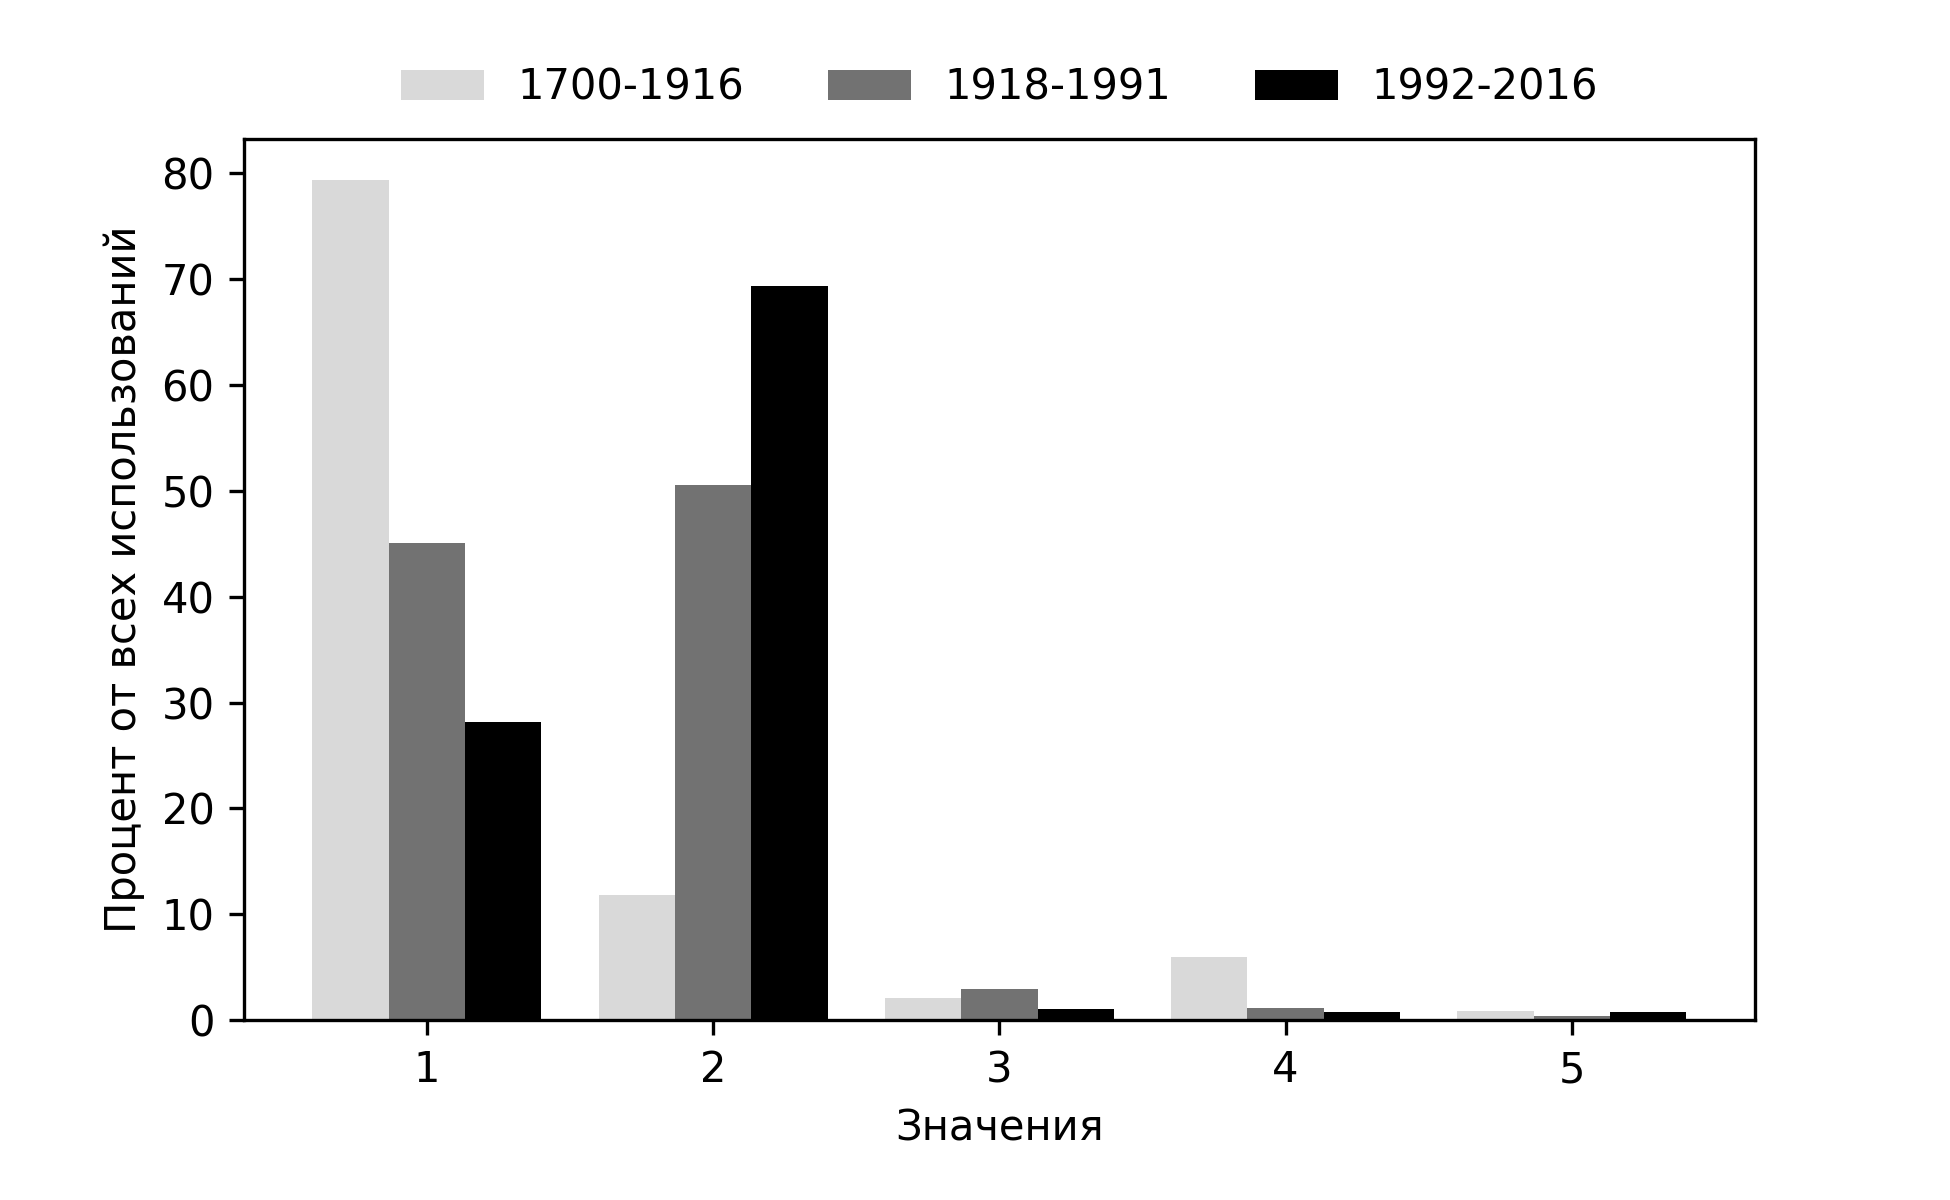
\includegraphics[width=0.8\textwidth]{img/visualizations/mashina_minimal}
	\caption{Изменение значений слова \textit{машина}}
	\label{fig:Машина_example}
\end{figure}

Значения для визуализации слова \textit{машина} (Параметры: eps=0.14, min\_samples=5).

\begin{enumerate}
    \item Приспособление, устройство, служащее для выполнения какой-л. работы.
    \item Автомобиль, транспортное средство.
    \item Самолет, вертолет и т. п.
    \item О человеке, действующем механически, бездумно.
    \item Система, совокупность каких-либо учреждений, организаций, предприятий и т. п.
\end{enumerate}

%\begin{FIGURE}[H]{Изменение значений слова \textit{свалка} \label{fig:example-figure-2}}
%	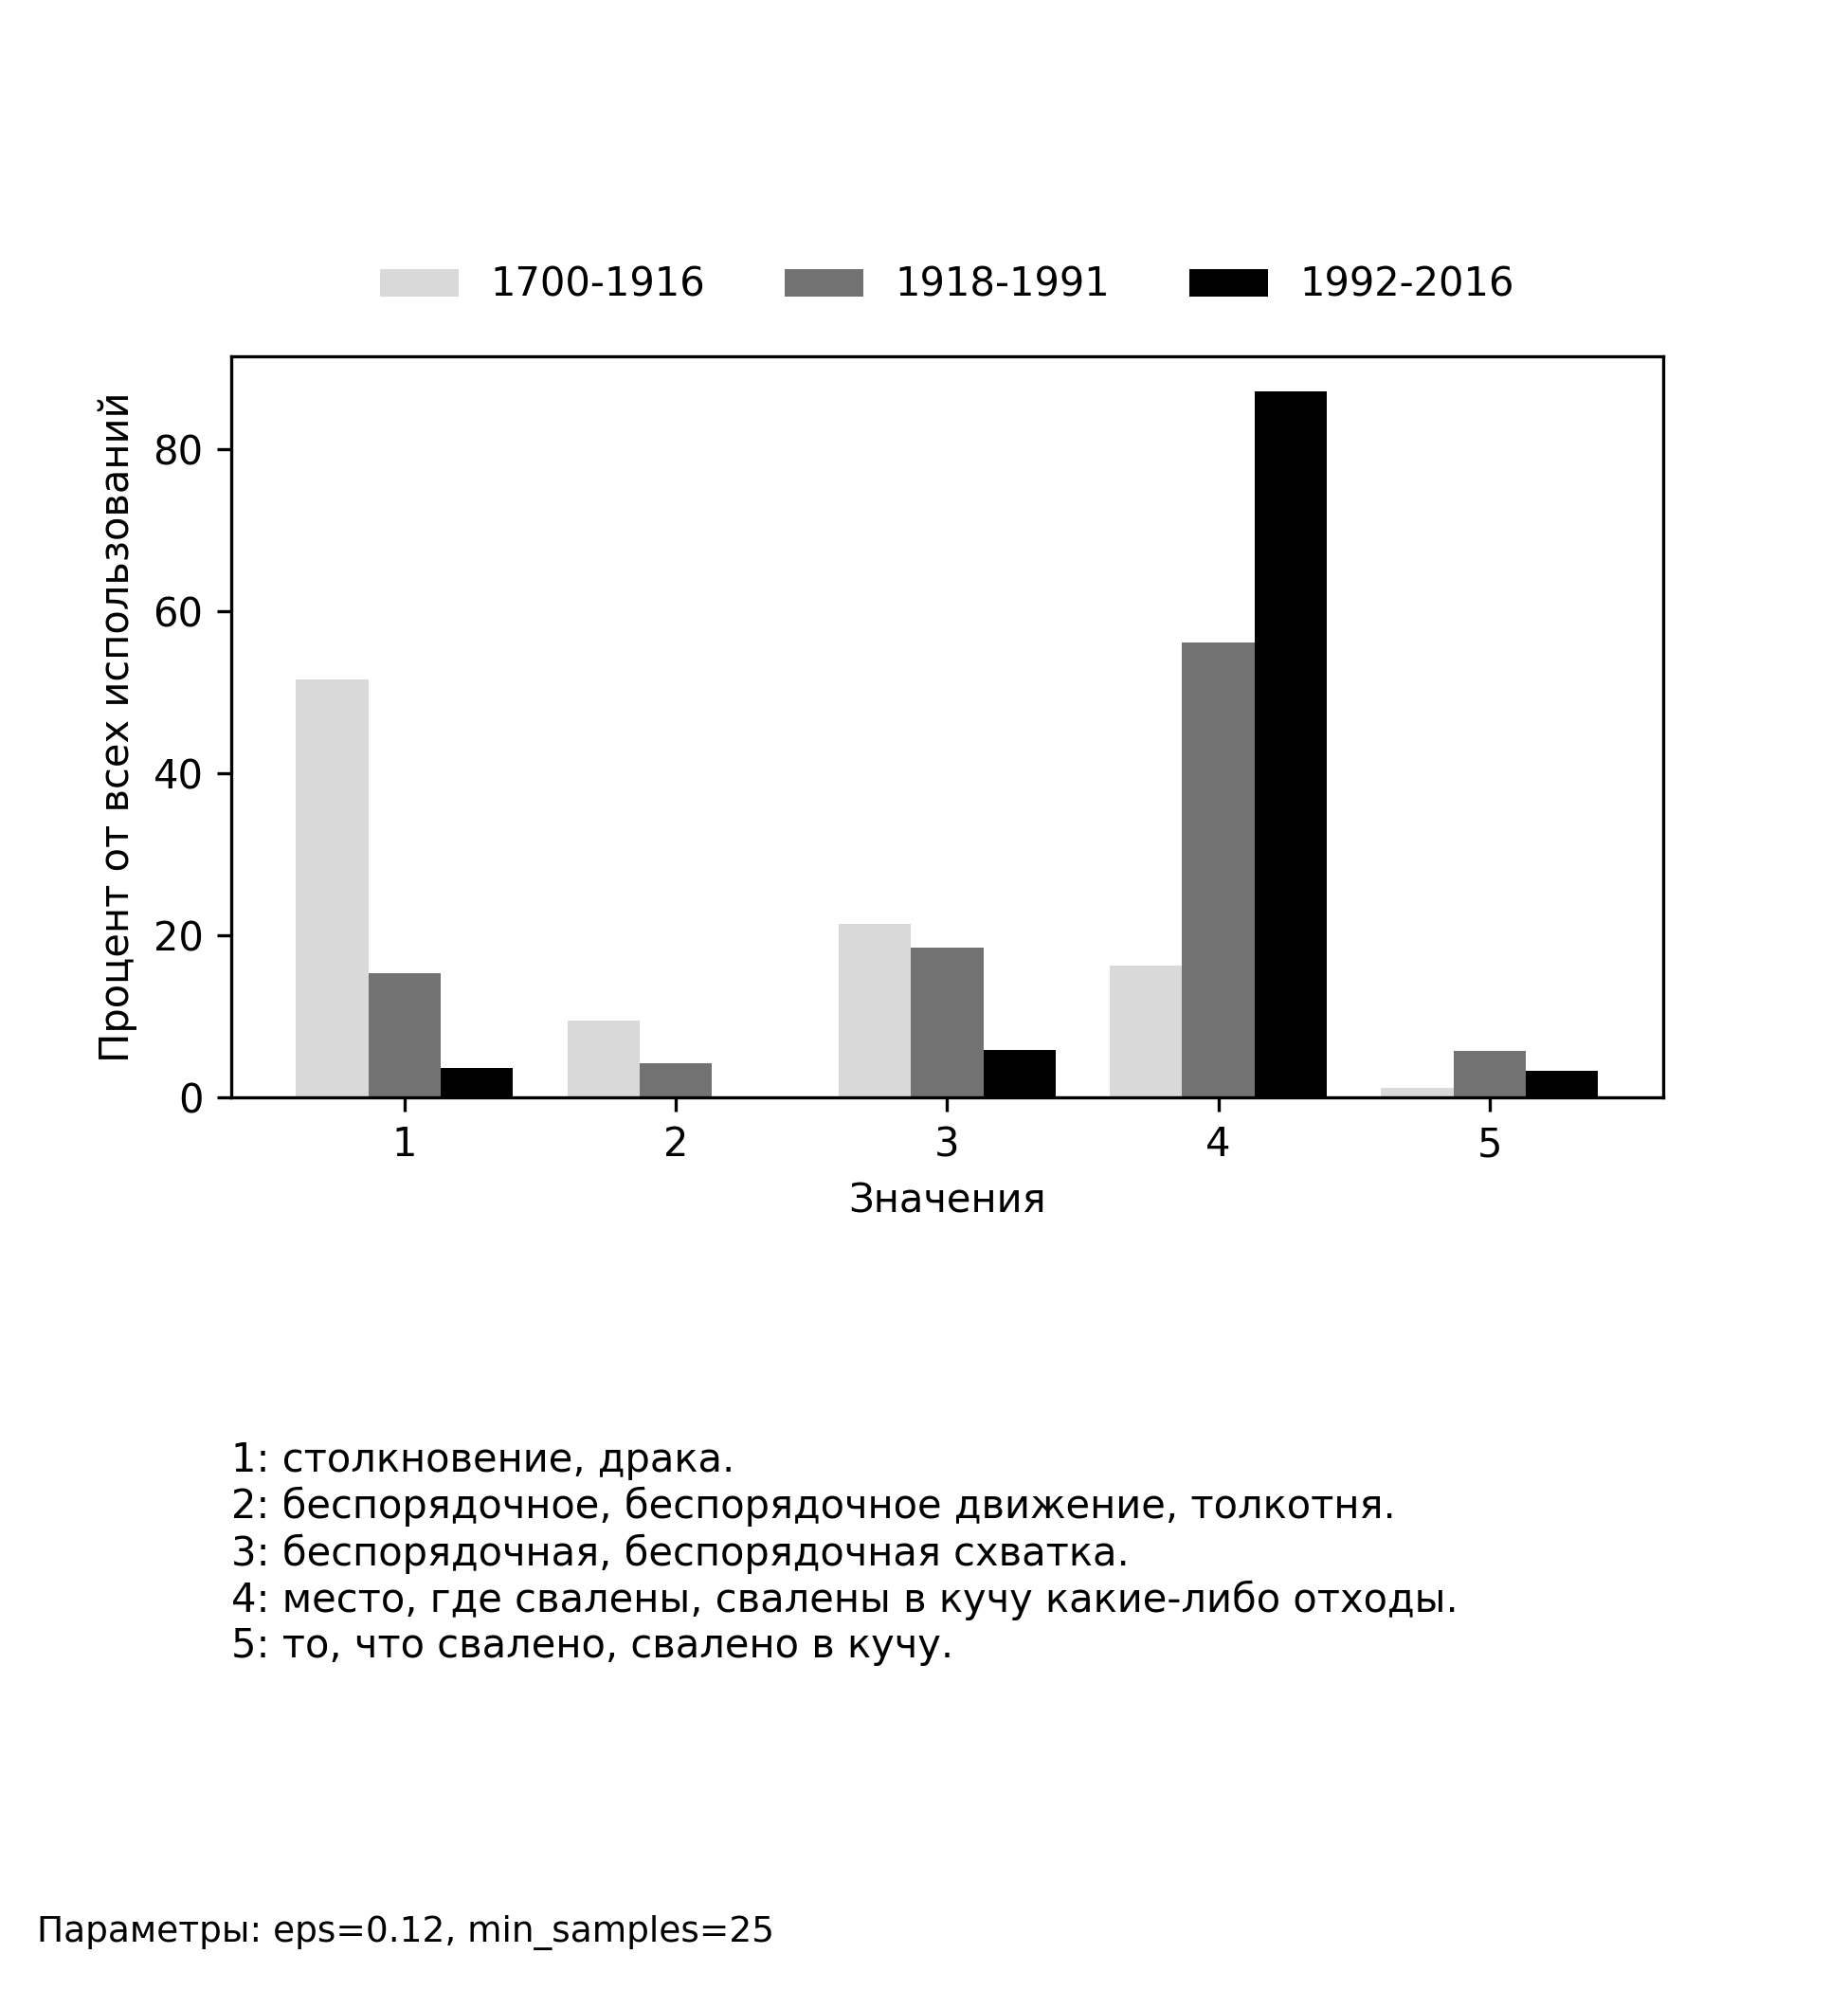
\includegraphics[width=0.75\textwidth]{img/visualizations/svalka}
%\end{FIGURE}

\section{Код работы}

Код, использованный во время выполнения настоящей работы, выложен в открытый доступ
на сайте GitHub.~\citeurl{WorkGitHub}

Проект включает в себя 3277 строки кода на языке python3.11, % (+1156 викисловарь в мейне (всего 4433) или +1277 в бранче)
481 строку скриптов на языке bash,
а также 562 строки документации. % (всего 703 в мейне, 719 с бранчем)

Проект включает следующие модули:
\begin{itemize}
    \item \textit{config}: Запуск тестов и проверок проекта с помощью CI
    \item \textit{latex}: Написание текста работы в формате LaTeX
    \item \textit{model}: Обучение модели и тестирование метриками
    \item \textit{mas\_parser}: Краулер и парсер словаря МАС
    \item \textit{vizvector}: Векторизация определений и визуализация результатов
    \item \textit{rushifteval}: Тестирование алгоритма на материале соревнования Rushifteval
    \item \textit{ruscorpora}: Позволяет осуществить качественный анализ алгоритма
\end{itemize}

Наличие тестов и открытого доступа к коду проекта позволяет
сделать исследование воспроизводимым, а также готовым к внедрению в другие проекты.

\section{Качественный анализ результатов работы алгоритма}

Для дальнейшего анализа результатов алгоритма используются 20 слов с изменившемся
значением из книги «Два века в двадцати словах»~\cite{TwoCenturies}:
\textit{знатный}, \textit{кануть}, \textit{классный}, \textit{мама}, \textit{машина}, \textit{молодец},
\textit{пакет}, \textit{передовой}, \textit{пионер}, \textit{пожалуй}, \textit{пока}, \textit{привет},
\textit{пружина}, \textit{публика}, \textit{свалка}, \textit{сволочь},
\textit{стиль}, \textit{тётка}, \textit{тройка}, \textit{червяк}.
Использования данных слов взяты из диахронического корпуса НКРЯ.

Для каждого рассматриваемого слова из каждого периода (досоветсткий, советский и постсоветсткий)
берётся выборка из 300 вхождений,
где для каждого использования слова генерируется определение, а после строится соответствующая визуализация.

Далее для каждого слова описана семантика слов на основе словарей в соответствии
с рекомендациями издания И.А. Стернина~\cite{SemanticDefinitionsAndAnalysis}.
В соответствии с ними, так как невозможно построить полное описание значения слова
с использованием только одного словаря, требуется обобщение данных нескольких словарей.
В качестве материала взяты три словаря современного русского языка
«Большой толковый словарь» (\textit{БТС})~\cite{TolkovyKuznetsov},
«Толковый словарь русского языка Дмитриева» (\textit{ТСД})~\cite{TolkovyDmitriev} и
«Толковый словарь русского языка» Ожегова и Шведовой (\textit{ТСО}),
а также книга «Два века в двадцати словах».
Книга «Два века в двадцати словах» использована при обобщении значений,
поскольку наряду со словарями содержит описания значений.
Исключением при обобщении значения является информация из помет,
так как модель не обучалась на их генерацию.
После чего проведено сравнение выявленных при семантическом описании лексемы
значений и тех, что выявлены алгоритмом визуализации.

Кроме того, произведено сравнение статистической информации по использованию слов
в разные периоды для значений, соотносимых со значениями из книги
«Два века в двадцати словах».

Следует учитывать то, что в книге исследуются периоды длиной меньше, чем в настоящей работе.
Например, вместо досоветского выделяют 1800-1849, 1850-1874, 1875-1899, а также 1900-1924,
в связи с чем не представляется возможным выявить изменения между короткими периодами из книги.

Определения оцениваются по классификации, описанной в Главе 1 и построенной на основе работ~\cite{huang-etal-2021-definition} и~\cite{noraset2016definition}.

Далее представлен разбор результата работы предлагаемого подхода для 3 слов, чьи результаты анализа
значительно отличаются друг от друга.
После этого представлены общие выводы по качественному анализу.

Подробный анализ результатов по каждому из остальных 17 слов представлен в Приложении А.

%\section*{Свалка}
%
%\subsection*{Семантическое описание лексемы \textit{Свалка} по словарям}
%
%В результате анализа семем лексемы \textit{свалка} в толковых словарях были
%выделены семь групп значений, которые можно условно сформулировать
%следующим образом:
%
%\begin{enumerate}
%    \item Место для сбора мусора, нечистот.
%(\textit{«Место, куда свозят, выбрасывают мусор, нечистоты, негодные вещи.»} в БТС,
%\textit{«Место, куда вывозят, выбрасывают мусор, нечистоты, негодные вещи.»} в ТСД,
%\textit{«Место для сбора мусора, нечистот»} в «Двух веках в двадцати словах»)
%    \item Процесс сваливания.
%(\textit{«к Свалить»} в БТС,
%\textit{«Процесс сваливания»} в «Двух веках в двадцати словах»)
%    \item Всеобщая драка.
%(\textit{«Свалкой называют всеобщую драку, в которой участвует много людей»} в ТСД,
%\textit{«Драка»} в «Двух веках в двадцати словах»)
%    \item Скопление людей, толпа.
%(\textit{«Скопление людей, толпа.»} в «Двух веках в двадцати словах» и в БТС)
%    \item Груда, куча, нагромождение чего-либо.
%(\textit{«Беспорядочно накиданная груда, куча чего-л.»} и
%\textit{«Если кто-либо превращает квартиру в свалку, то это означает, что там в беспорядке нагромождаются предметы, мебель и пр.»} в БТС,
%\textit{«Свалкой называют беспорядочно накиданную груду каких-либо предметов.»} в ТСД,
%\textit{«Груда»} в «Двух веках в двадцати словах»)
%    \item Вооруженное столкновение войск, битва.
%(\textit{«Битва»} в «Двух веках в двадцати словах»)
%\end{enumerate}

%\subsection*{Результат алгоритма}
%
%\begin{figure}[H]
%	\centering
%	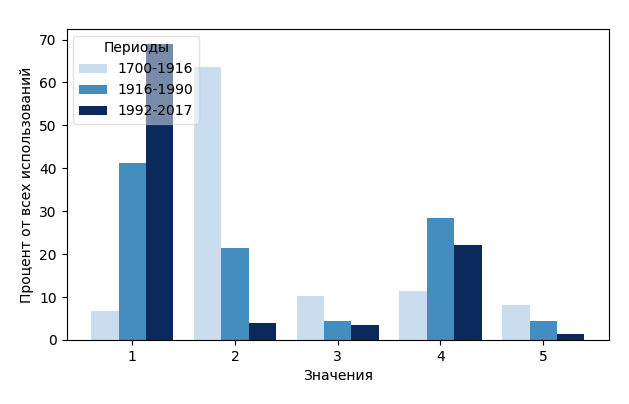
\includegraphics[width=0.8\textwidth]{img/Words_Meanings/Свалка (Больше значений)}
%	\caption{Изменение значений слова \textit{Свалка} (Параметры: eps=0.9, min\_samples=50)}
%	\label{fig:Свалка}
%\end{figure}
%
%%\begin{figure}[H]
%%	\centering
%%	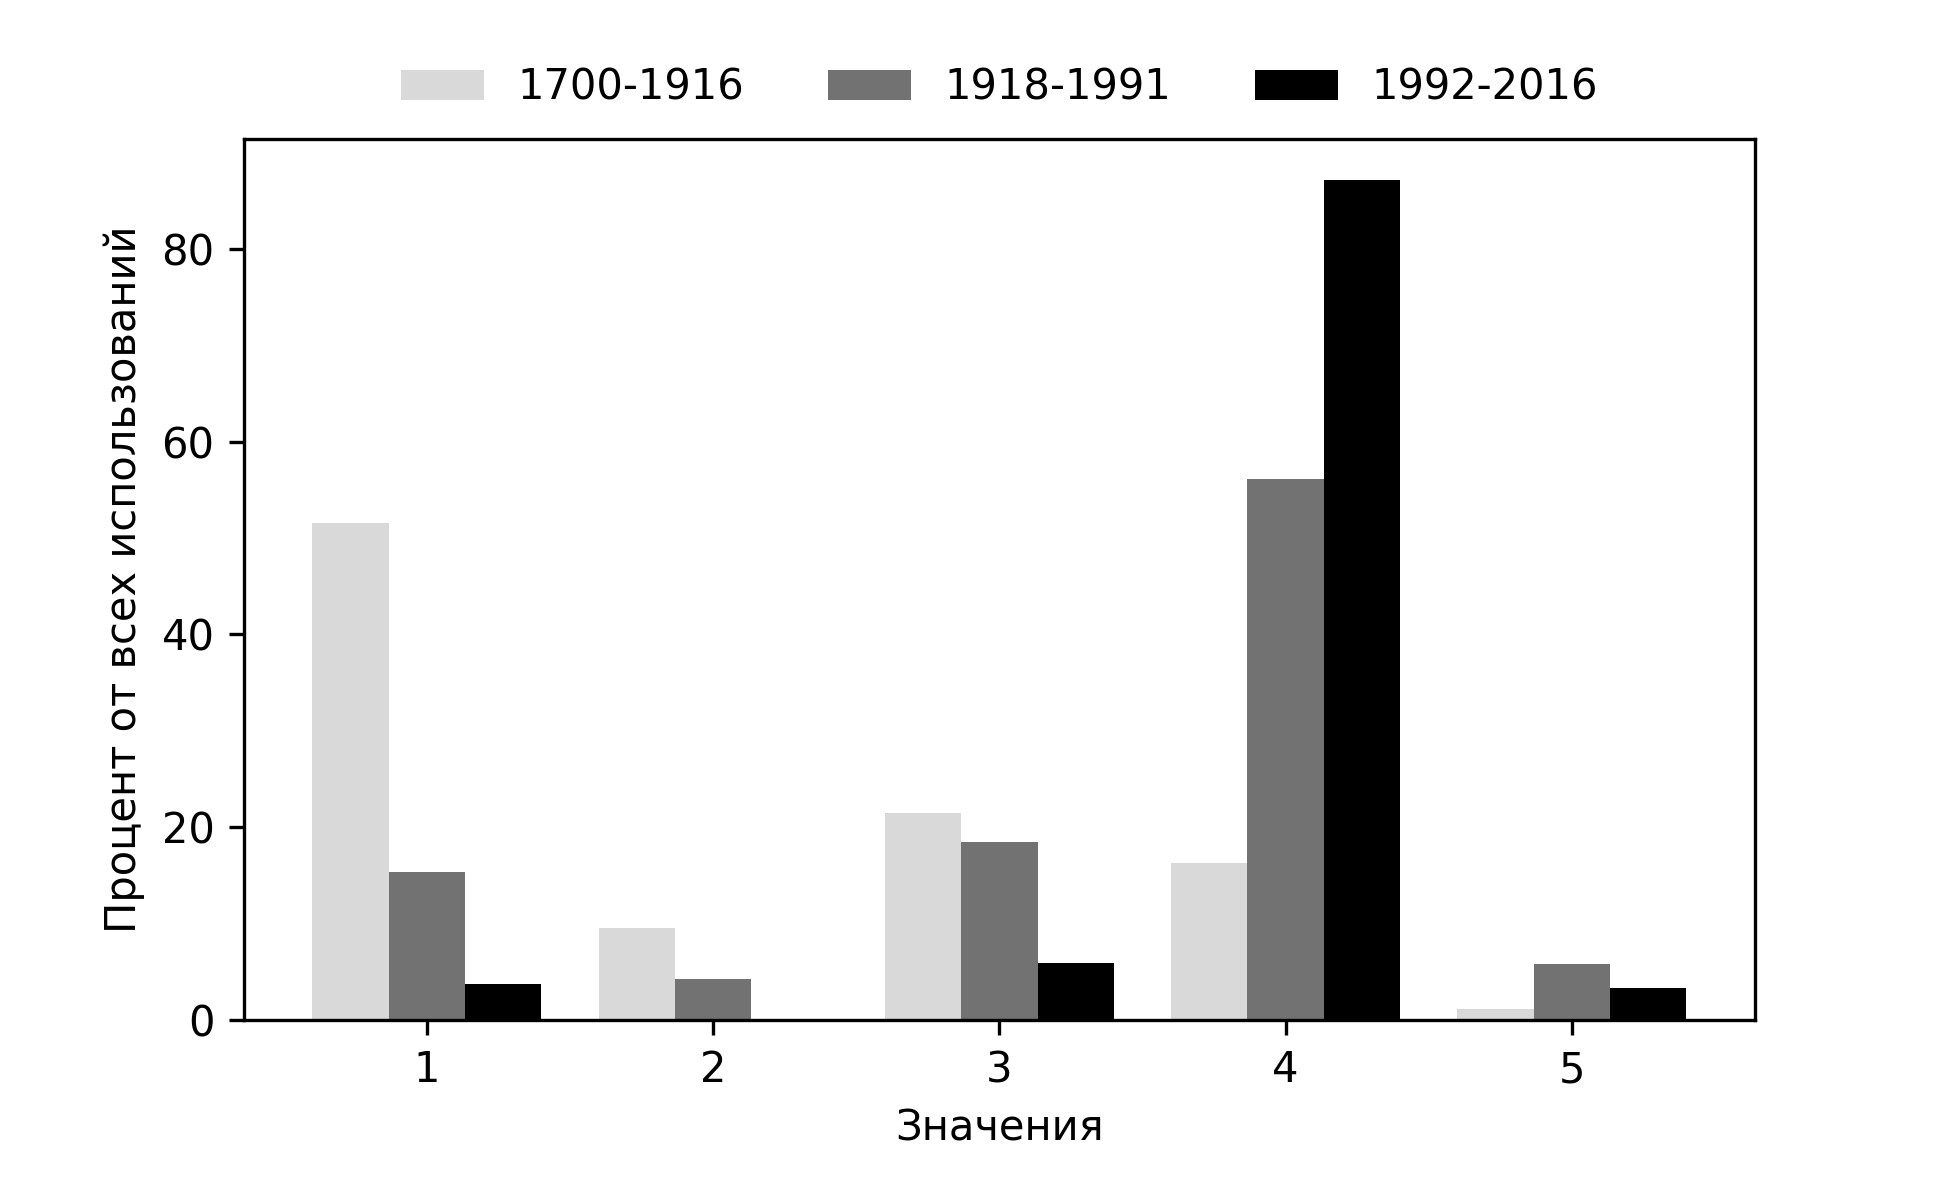
\includegraphics[width=0.8\textwidth]{img/visualizations/svalka_minimal}
%%	\caption{Изменение значений слова \textit{Свалка} (Параметры: eps=0.9, min\_samples=50)}
%%	\label{fig:Свалка}
%%\end{figure}
%
%Значения для визуализации слова \textit{Свалка}:
%
%\begin{enumerate}
%    \item Место, куда свозят, сваливают мусор, отходы.
%    \item Столкновение, драка.
%    \item Беспорядочное скопление кого-либо, чего-либо.
%    \item Место, где свалены, нагромождены какие-л. предметы.
%    \item Беспорядочное, беспорядочное скопление людей.
%\end{enumerate}
%
%%\begin{enumerate}
%%    \item Столкновение, драка.
%%    \item Беспорядочное, беспорядочное движение, толкотня.
%%    \item Беспорядочная, беспорядочная схватка.
%%    \item Место, где свалены, свалены в кучу какие-либо отходы.
%%    \item То, что свалено, свалено в кучу.
%%\end{enumerate}
%
%\subsection*{Анализ результатов}
%
%Первые четыре определения корректно сформулированы.
%Пятое имеет повторение слова «беспорядочное» – ошибку в генерации определения.
%Далее мы будем считать это определение как «Беспорядочное скопление людей.».
%
%Три определения имеют явные аналоги в составленном ранее описании значений слова.
%’Место, куда свозят, сваливают мусор, отходы.’ имеет с
%’Место, куда свозят, выбрасывают мусор, нечистоты, негодные вещи.’
%общие смысловые элементы:
%«место», «своз/сваливание», «отходы/нечистоты».
%
%’Столкновение, драка.’ соответствует определению
%’Всеобщая драка, потасовка.’,
%хоть в словаре оно и более узкое из-за наличия помимо смыслового элемента
%«драка» семы «всеобщности».
%
%’Беспорядочное скопление людей.’ имеет аналог
%’Скопление людей, толпа.’.
%Здесь общие семы «скопление», «люди», хоть и имеется дифференциальная сема «беспорядочности»,
%делающая определение алгоритма более узким.
%
%’Место, где свалены, нагромождены какие-л. предметы.’ близко к
%’Беспорядочно накиданная груда, куча чего-л.’
%Общими семами являются
%«нагромождение», «предметы», однако не акцентируется
%«беспорядочность» явно, вместо этого эта сема присутствует в значениях слова
%«нагромождены» («Нагромоздить –
%построить в чрезмерно большом количестве, очень тесно или в беспорядке.»).
%
%Также алгоритм предлагает более общее значение
%’Беспорядочное скопление кого-либо, чего-либо.’,
%которое может включать как живые, так и неживые объекты, объединяя
%значения ’Скопление людей, толпа.’ и ’Груда, куча, нагромождение чего-либо.’
%
%Алгоритм не предлагает значение ’Процесс сваливания’.
%В этом случае акцентируется действие «свалить», указывающее на процесс перемещения
%предметов/материала с целью создания свалки.
%Однако, это значение не вынесено отдельно ни в одном периоде в «Двух веках в двадцати словах»
%и является редким, что могло быть причиной отсутствия в визуализации.
%
%Кроме того, в визуализации отсутствует значение ’Битва’,
%которое указывается как преобладающее для периода до 1850 года.
%В предсказаниях модели присутвуют примеры с этим значением,
%однако их количество в исследуемом материале незначительно,
%поэтому оно не вошло в визуализацию.
%Например, для \textit{«Но в свалке, как обыкновенно действует кавалерия, сабля или палаш лучше»}
%было сгенерировано определение
%’Бой, в котором участвуют несколько противников’.
%
%%Турки стали отступать после сильной свалки, но, получив подкрепление и пользуясь своим превосходством (пушки и конница), перешли было опять в наступление.
%%Беспорядочное столкновение, бой.
%
%Перейдем к частотности значений.
%
%В книге «Два века в двадцати значениях» как появившееся в 1900-ых годах указано
%значение \textit{«Место для сбора мусора, помойка.»}, соответствующее первому значению,
%предложенному алгоритмом ’Место, куда свозят, сваливают мусор, отходы.’.
%Как видно из графика результатов алгоритма, оно почти не используется в досоветский период,
%но становится главным
%с 40\% использования в советский период и доминирует в постсоветский с около 70\%.
%Эти данные совпадают с тем, что говорится в книге, где утверждается 87\% использования
%значения \textit{«Помойка.»} в 1998-1997 годы, 32\% для 1925-1949 годов.
%
%Уменьшается же судя по графику преимущественно значение 2 (’Столкновение, драка.’),
%которое падает с 65\% использований в досоветский период до 5\% в постсоветский.
%В книге резульаты схожи.
%Так, утверждается, что в 1875-1899 году слово имело значение ’Драка.’
%в 71\% использований,
%а к 1998-1997 значение упало до 12\%.
%
%\noindent % Prevents indentation for this line to align the images at the left margin
%\begin{figure}[H]
%    \centering % Centers the images
%    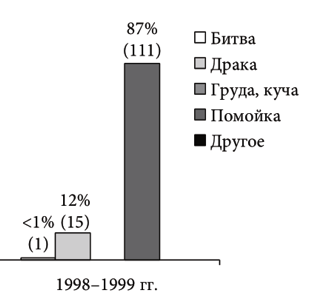
\includegraphics[width=0.32\textwidth]{img/book/Свалка 1998-1999}
%    \hfill % Fills the space between the images
%    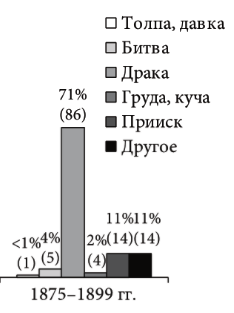
\includegraphics[width=0.32\textwidth]{img/book/Свалка 1875-1799}
%    \hfill % Fills the space between the images
%    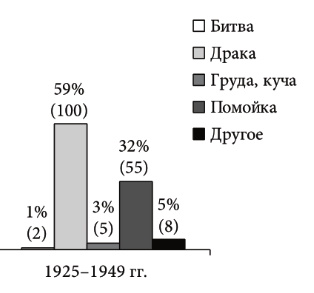
\includegraphics[width=0.32\textwidth]{img/book/Свалка 1925-1949}
%    \caption{Визуализации для слова "Свалка" из книги "Два века в двадцати словах".}
%\end{figure}
%
%Таким образом, модель довольно точно отражает реальное изменение значений слова «свалка»
%во времени, согласуясь с данными из толкового словаря и историческим исследованием.
%Она адекватно выделяет как наиболее широко используемое сегодня значение,
%связанное с местом сбора мусора,
%так и менее очевидные значения, включая драку и беспорядочное скопление предметов или людей.

\subsection*{Анализ слова \textit{тройка}}

В результате анализа семем лексемы \textit{тройка} в толковых словарях были выделены девять значений,
которые можно сформулировать следующим образом:

\begin{enumerate}
    \item Количество три. \textit{Тройка поплавков.}
    (\textit{«Количество три.»} в БТС,
    \textit{«Тройное количество чего-либо.»} в ТСД,
    \textit{«(о сходных или однородных предметах) количество три.»} в ТСО,
    \textit{«Количество, сумма из трех единиц.»} в «Двух веках в двадцати словах»)

    \item Оценка успеваемости в пятибалльной системе, означающая удовлетворительно. \textit{Учиться на тройки.}
    (\textit{«Оценка успеваемости в пятибалльной системе, означающая удовлетворительно.»} в БТС,
    \textit{«Школьная учебная отметка «удовлетворительно»».} в ТСО,
    \textit{«В пятибалльной системе тройкой называют удовлетворительную, посредственную оценку чьих-либо знаний.»} в ТСД,
    \textit{«Оценка в учебе.»} в «Двух веках в двадцати словах»)

    \item Упряжка в три лошади. \textit{Русская тройка.}
    (\textit{«Три лошади в одной упряжке.»} в БТС,
    \textit{«Упряжка в три лошади.»} в ТСО,
    \textit{«Тройкой называют упряжку из трёх лошадей — коренной и двух пристяжных.»} в ТСД,
    \textit{«Лошади.»} в «Двух веках в двадцати словах»)

    \item Костюм, состоящий из пиджака (или жакета), брюк (или юбки) и жилета. \textit{Прийти в тройке.}
    (\textit{«Костюм, состоящий из пиджака (или жакета), брюк (или юбки) и жилета»} в БТС,
    \textit{«Костюм, состоящий из пиджака, брюк (или жакета, юбки) и жилета»} в ТСО,
    \textit{«Костюм, который состоит из пиджака (или жакета), брюк (или юбки) и жилета»} в ТСД,
    \textit{«Костюм»} в «Двух веках в двадцати словах»)

    \item Игральная карта с тремя очками. \textit{Играю тройками.}
    (\textit{«Игральная карта в три очка.»} в БТС,
    \textit{«В картах тройкой называют игральную карту в три очка»} в ТСД,
    \textit{«Игральная карта с тремя очками»} в «Двух веках в двадцати словах»)

    \item Цифра 3. \textit{Написать тройку.}
    (\textit{«Цифра 3»} в БТС,
    \textit{«Цифра 3»} в ТСО,
    \textit{«Тройка — это цифра 3»} в ТСД)

    \item Транспортное средство, обозначенное цифрой 3. \textit{Тройка изменила маршрут.}
    (\textit{«Название автобуса, трамвая, троллейбуса третьего маршрута»} в БТС,
    \textit{«Название чего-н. (обычно транспортного средства), обозначенного цифрой 3»} в ТСО,
    \textit{«Маршрут автобуса, трамвая, троллейбуса, который пронумерован цифрой 3»} в ТСД)

    \item Группа из трёх человек, обычно неразлучная. \textit{Тройка знатоков.}
    (\textit{«Тройкой называют устойчивую группу людей.»} в ТСД,
    \textit{«Три человека»} в «Двух веках в двадцати словах»)

    \item Звено боевых истребителей. \textit{Идёт в пикирование вторая тройка.}
    (\textit{«Тройкой называют звено боевых истребителей»} в ТСД)
\end{enumerate}

%Фразеологизмы:
%\begin{enumerate}
%    \item Пара-тройка.
%    (\textit{«Если кто-либо говорит о паре-тройке чего-либо, то это означает, что речь идёт об очень малом, незначительном количестве чего-либо»} в ТСД)
%
%    \item Первая тройка.
%    (\textit{«Если кто-либо, занимаясь какой-то деятельностью, входит в первую тройку, то это означает, что этот человек назван в числе трёх лучших специалистов, спортсменов и т. п.»} в ТСД)
%\end{enumerate}

\begin{figure}[H]
	\centering
	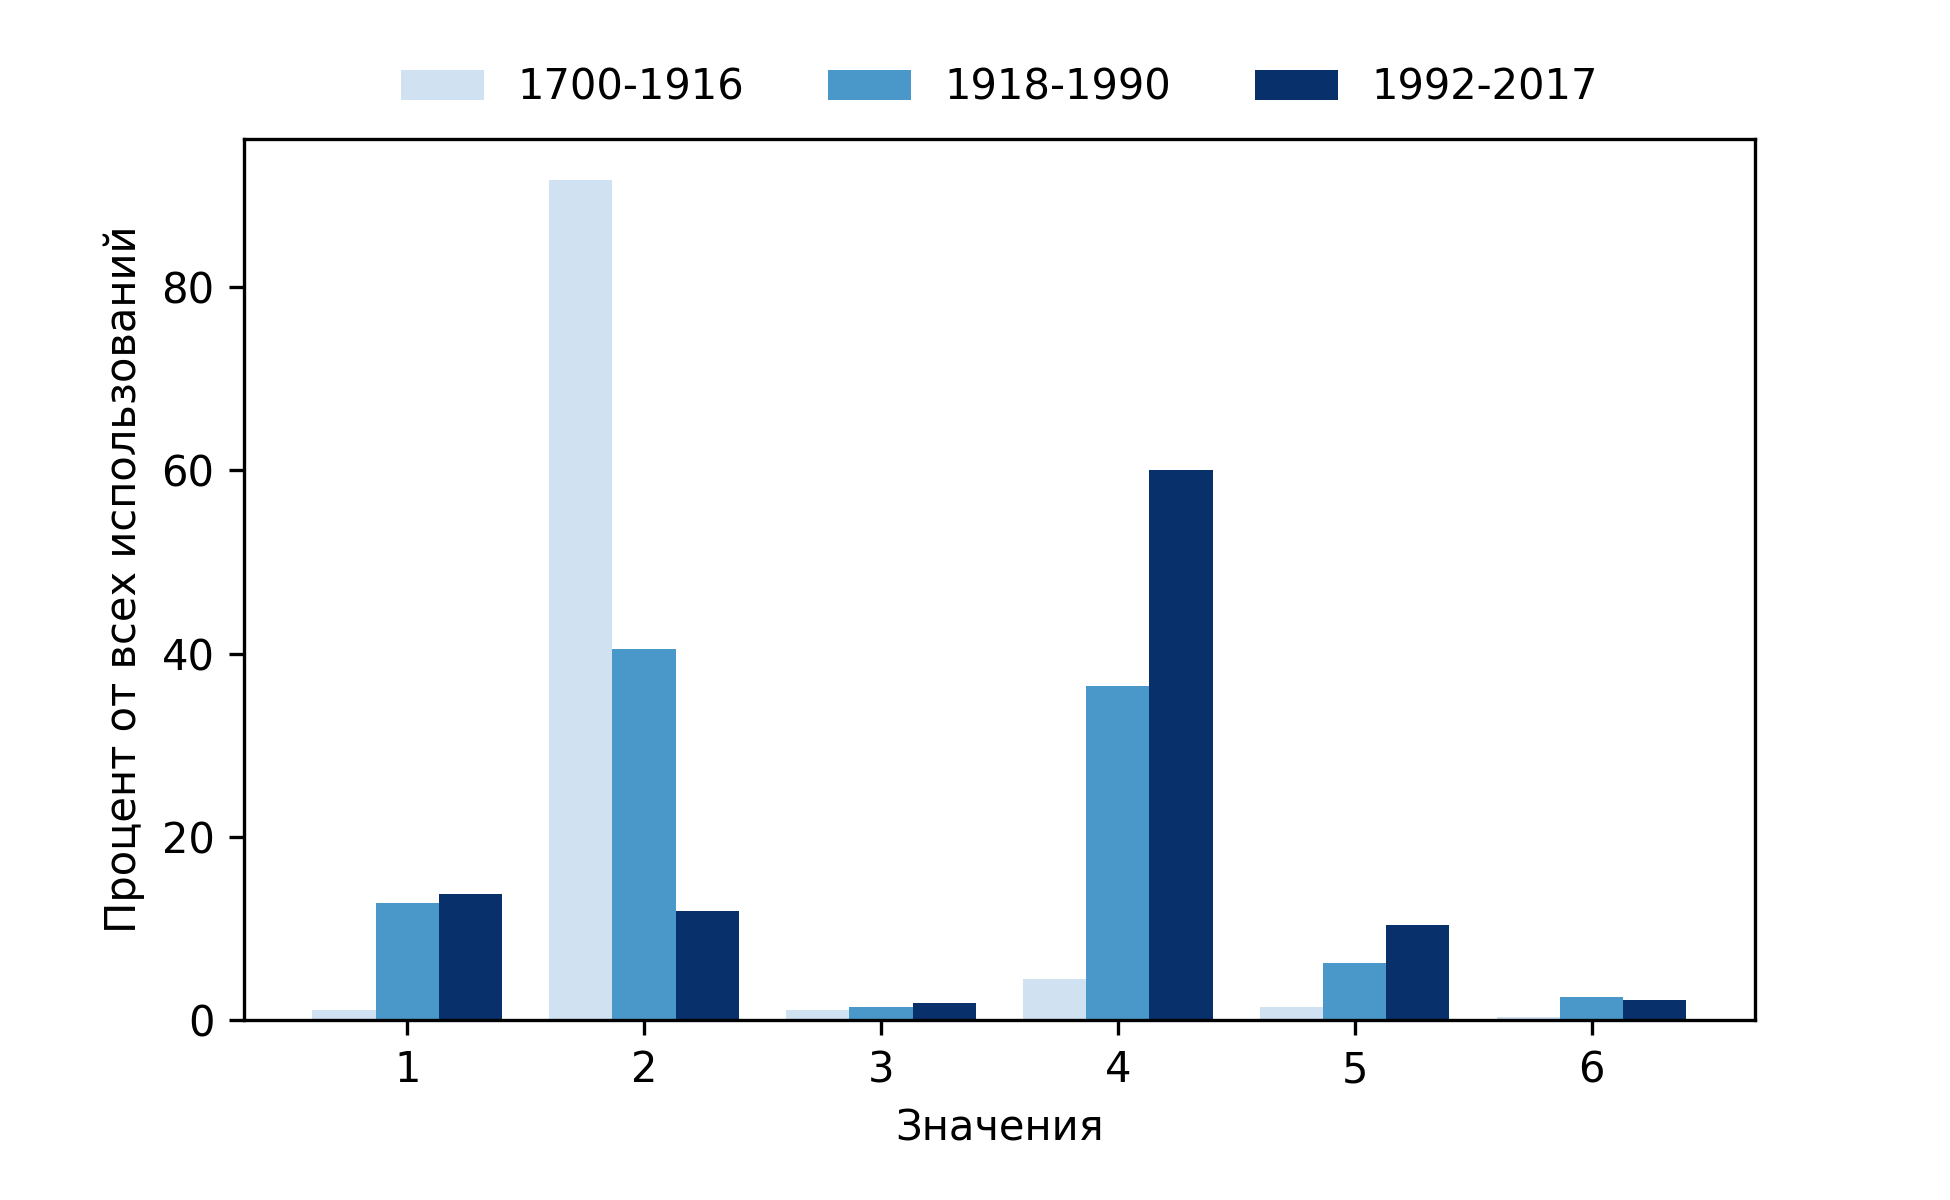
\includegraphics[width=0.8\textwidth]{img/visualizations/trojka_minimal}
	\caption{Изменение значений слова \textit{тройка}}
	\label{fig:Тройка}
\end{figure}

Визуализация для слова \textit{тройка} представлена на Рисунке~\ref{fig:Тройка}.
(Параметры: eps=0.28, min\_samples=12)
Соответствующие значения:
\begin{enumerate}
    \item Неудовлетворительная оценка по какому-либо предмету.
    \item Одна из трех лошадей, запряженных в такую повозку.
    \item Игральная карта с тремя одинаковыми мастями.
    \item Группа лиц, состоящая из трех лиц.
    \item Число 3.
    \item Старинная мужская верхняя одежда из сукна или бархата, застегивавшаяся спереди на пуговицы.
\end{enumerate}

\subsubsection*{Анализ значений слова \textit{тройка}}

Пятое определение корректно сформулировано.
Четвёртое определение избыточно.
Первое, второе, третье и шестое определения полностью не соответствуют обобщенным значениям.

\begin{itemize}
    \item ’Число 3.’ полностью соответствует ’Число 3’.
\end{itemize}

\begin{itemize}
    \item ’Неудовлетворительная оценка по какому-либо предмету.’ является близким значением,
так как в обобщенных значениях имеется ’школьная оценка’
(’Оценка успеваемости в пятибалльной системе, означающая удовлетворительно.’),
но она означает ’удовлетворительно’, а не ’неудовлетворительно’.

    \item ’Одна из трех лошадей, запряженных в такую повозку.’ является близким обобщённому
значению ’Упряжка в три лошади.’,
но формулировка «одна из трех лошадей» некорректна,
так как денотатом является упряжка, включающая в себя все три лошади и повозку.

    \item ’Игральная карта с тремя одинаковыми мастями.’ является близким значением,
так как в обобщенных значениях имеется игральная карта с тремя очками,
но формулировка «с тремя одинаковыми мастями» некорректна,
мастью же является одна из четырёх категорий карт (В БТС:
«Масть – один из четырёх разрядов на которые делится колода карт по цвету и форме очков.»).

    \item ’Группа лиц, состоящая из трех лиц.’ соответствует
’Группа из трёх человек, обычно неразлучная.’, так как включает те же семы \textit{’группа лиц’}, \textit{’три’},
однако содержит повторение слова \textit{лиц}, которое делает его избыточным.

    \item ’Старинная мужская верхняя одежда из сукна или бархата, застегивавшаяся спереди на пуговицы.’
является некорректным определением, так как такое описание больше соответствует
историческим видам одежды, таким как кафтан или сюртук, но не «костюму»,
представляющему собой комплект из брюк, пиджака и жилета.
\end{itemize}

Обобщённые значения, не найденные в визуализации:
\begin{itemize}
    \item ’Цифра 3.’ отсутствует среди предложенных моделью значений.  % TODO: привести генерацию
%Можно предположить, что информации из контекста использований недостаточно для выделения этого значения.
Можно предположить, что модель могла не выделить это значение из-за ограниченного количества использований.

    \item ’Транспортное средство, обозначенное цифрой 3.’ также отсутствует в визуализации.
%Однако, модель способна на выделение данного значения.  % TODO: привести генерацию

    \item ’Звено боевых истребителей.’ отсутствует среди предложенных моделью значений.  % TODO: привести генерацию
Модель, вероятно, могла не выделить это значение из-за ограниченного количества использований.
\end{itemize}

Таким образом, для лексемы \textit{тройка} представлено 1 корректное определение.
Среди ошибок присутствуют:
\begin{itemize}
    \item Избыточность или чрезмерное использование общих фраз: 1
    \item Некорректность: 1
    \item Близкое значение: 3
\end{itemize}

Перейдем к частотности значений.

Судя по книге «Два века в двадцати словах»,
данные которой представлены на Рисунках~\ref{fig:TwoCenturiesTrojka1} и~\ref{fig:TwoCenturiesTrojka2}, в XIX веке для слова \textit{тройка}
преимущественным является значение ’Упряжка в три лошади.’ с около 95\% использований,
что также отражено в нашей визуализации с около 90\% использований близкого значения
’Одна из трех лошадей, запряженных в такую повозку.’
Начало советского периода, утверждается в книге, характерно увеличением использования значения
’Три человека’ в 20-ые годы, а также ’Оценка успеваемости в пятибалльной системе, означающая удовлетворительно.’
в 40-ые годы.
К концу советского периода используется множество значений и
’Упряжка в три лошади.’ больше не является
лидирующим.
Это информация отражена в нашей визуализации, где ’Одна из трех лошадей, запряженных в такую повозку.’
падает до 40\% в советское время и 15\% постсоветское.
Вместо него самым частым становится ’Группа лиц, состоящая из трех лиц.’ с около 60\%
в постсоветский период, а также частыми становятся значения школьной оценки
и числа 3 с 10-15\% использования.

\noindent % Prevents indentation for this line to align the images at the left margin
\begin{figure}[H]
    \centering % Centers the images
    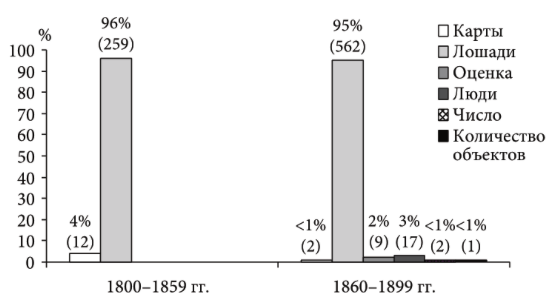
\includegraphics[width=0.8\textwidth]{img/book/trojka/1800-1899}
    \caption{Значения слова \textit{тройка} для 1800-1899 согласно~\cite{TwoCenturies}}
    \label{fig:TwoCenturiesTrojka1}
\end{figure}

\begin{figure}[H]
    \centering % Centers the images
    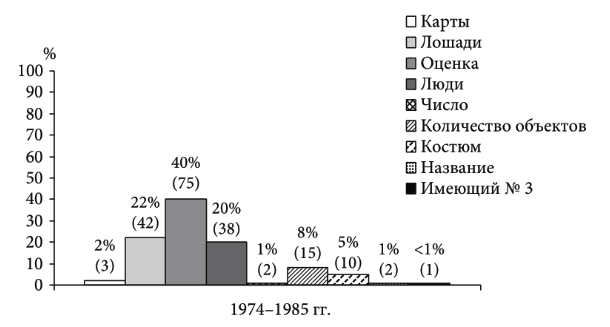
\includegraphics[width=0.8\textwidth]{img/book/trojka/1974-1985}
    \caption{Значения слова \textit{тройка} для 1974-1985 согласно~\cite{TwoCenturies}}
    \label{fig:TwoCenturiesTrojka2}
\end{figure}

Таким образом, предложенный подход по большей части отражает значения, в которых использовалось
слово \textit{тройка}, не полностью согласуясь с данными из толкового словаря,
но соответствуя историческим исследованием.

\subsection*{Анализ значений слова \textit{пока}}

\begin{enumerate}
    \item В течение некоторого времени; до сих пор ещё; впредь до чего-л. \textit{Пока ничего не известно.}
(\textit{«В течение некоторого времени; до сих пор ещё; впредь до чего-л.»} в БТС,
\textit{«В течение нек-рого времени, впредь до чего-н.; до сих пор еще.»} в ТСО,
\textit{«Наречие – в течение некоторого времени, до сих пор еще.»} в «Двух веках в двадцати словах»)

    \item В то время как. \textit{Пока он учится, надо ему помочь.}
(\textit{«В то время как; до того времени как.»} в БТС,
\textit{«В течение того времени как.»} в ТСО,
\textit{«Союз с фоновым значением ("в то время как").»} в «Двух веках в двадцати словах»)

    \item До того времени как. \textit{Пока солнце не взойдёт, на траве лежит иней.}
(\textit{«В то время как; до того времени как.»} в БТС,
\textit{«Союз с предельным значением ("вплоть до того как").»} в «Двух веках в двадцати словах»)

    \item Употребляется при прощании, до свидания. \textit{Ну, я пошел, пока!}
(\textit{«Приветствие при прощании, до свидания.!»} в ТСО,
\textit{«Элемент формулы прощания.»} и \textit{«Этикетное слово — до свидания.»} в «Двух веках в двадцати словах»)
\end{enumerate}

\begin{figure}[H]
	\centering
	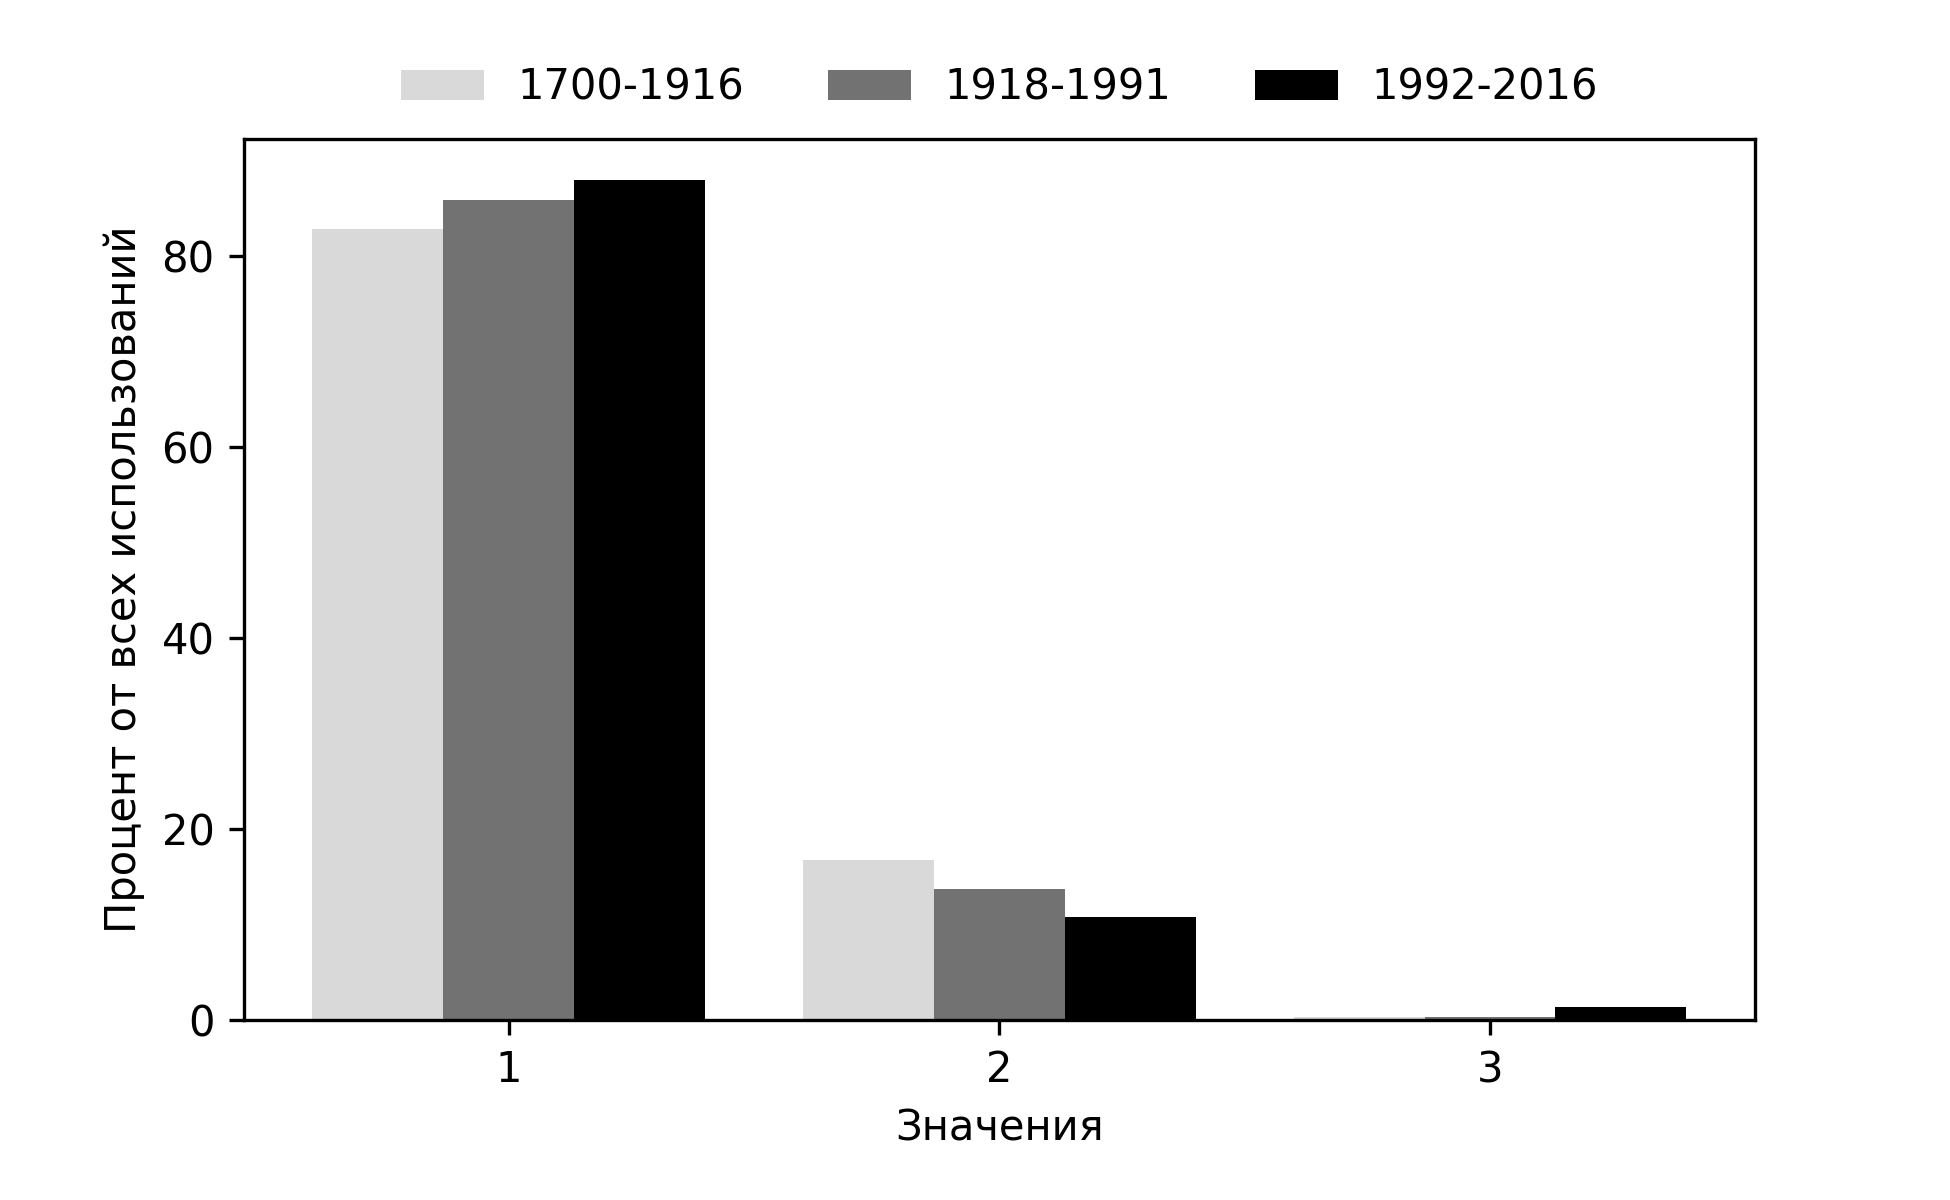
\includegraphics[width=0.8\textwidth]{img/visualizations/poka_minimal}
	\caption{Изменение значений слова \textit{пока}}
	\label{fig:Пока}
\end{figure}

Значения для визуализации слова \textit{пока} (Параметры: eps=0.25, min\_samples=5).

\begin{enumerate}
    \item В настоящее время, до тех пор.
    \item Употребляется при обозначении времени, в течение которого совершается действие.
    \item Употребляется при прощании с кем-л.
\end{enumerate}

\subsubsection*{Анализ значений слова \textit{пока}}

Первое, второе и третье определения корректно сформулированы.

\begin{itemize}
    \item ’В настоящее время, до тех пор.’ имеет общий смысловой элемент с
’В течение некоторого времени; до сих пор ещё; впредь до чего-л.’,
а именно семы \textit{’время’}, \textit{’до сих пор’}, \textit{’в течение’}.

    \item ’Употребляется при обозначении времени, в течение которого совершается действие.’ полностью соответствует
’В то время как.’, так как включает те же семы \textit{’время’}, \textit{’совершение действия’}.

    \item ’Употребляется при прощании с кем-л.’ полностью соответствует
’Употребляется при прощании, до свидания.’, так как включает те же семы \textit{’прощание’}, \textit{’до свидания’}.
\end{itemize}

Обобщённые значения, не найденные в визуализации:
\begin{itemize}
    \item ’До того времени как.’ отсутствует среди предложенных моделью значений.
Это значение близко к ’В то время как’, но с акцентом на предельность времени,
что могло привести к отсутствию этого значения в визуализации.
\end{itemize}

Таким образом, для лексемы \textit{пока} представлены 3 корректных определения.

Перейдем к частотности значений.

В книге, данные которой представлены на Рисунке~\ref{fig:TwoCenturiesPoka}, сообщается,
что изначальным и всегда преобладающим было использование слова в качестве
союза, после чего в XIX веке появилось использование как наречие, а затем в советский период
– как этикетное слово.
Данные из визуализации предложенного подхода поддерживают появление значения
’Употребляется при прощании с кем-л.’
поздно – несколько процентов для постсоветского периода, однако данные для наречия и союза
не совпадают.
Можно предположить, что модели сложно различать эти значения из-за их схожести.
Например, для
\textit{«Когда мы забирали щенка, нас предупредили, что ей категорически нельзя наверх забираться,
пока у нее слабые лапы.»}
было сгенерировано ’В настоящее время, до тех пор.’,
что относит его к наречию,
но из примера видно, что \textit{пока} связывает части предложения и является союзом.

\begin{figure}[H]
    \centering % Centers the images
    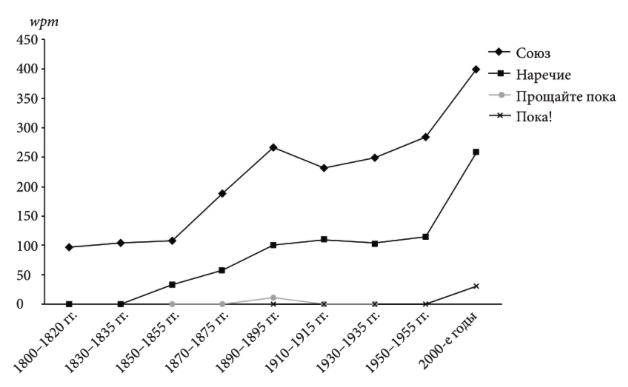
\includegraphics[width=0.8\textwidth]{img/book/poka/all}
    \caption{Значения слова \textit{пока} согласно~\cite{TwoCenturies}}
    \label{fig:TwoCenturiesPoka}
\end{figure}

Таким образом, предложенный подход лишь по большей части не отражает значения, в которых использовалось
слово \textit{пока}, так как из 3 выделенных значений, хоть и правильно сформулированных,
статистика использования не согласуется с данными книги.

\subsection*{Анализ значений слова \textit{пакет}}

\begin{enumerate}
    \item Упакованный в бумажную или иную обёртку какой-л. предмет (предметы); свёрток. \textit{Пакет сахарного песка.}
(\textit{«Упакованный в бумажную или иную обёртку какой-л. предмет (предметы); свёрток.»} в БТС,
\textit{«Бумажный сверток, упаковка с чем-н.»} в ТСРЯ,
\textit{«Предмет, который завёрнут в бумажную или другую упаковку.»} в ТСД,
\textit{«Упаковка, сверток»} в «Двух веках в двадцати словах»)

    \item Конверт с письмом официально-делового содержания. \textit{Он вскрыл пакет и углубился в чтение.}
(\textit{«Конверт с письмом официально-делового содержания.»} в БТС,
\textit{«Конверт с письмом официального назначения.»} в ТСРЯ,
\textit{«Конверт с письмом официально-делового содержания.»} в ТСД,
\textit{«Письмо, конверт, почтовое отправление»} в «Двух веках в двадцати словах»)

    \item Бумажный или полиэтиленовый мешок для упаковки каких-л. предметов, продуктов и т.п. \textit{Продажа овощей в пакетах.}
(\textit{«Бумажный кулёк для упаковки каких-л. предметов, продуктов и т.п.»} в БТС,
\textit{«Бумажный мешок для продуктов, кулек.»} в ТСРЯ,
\textit{«Бумажный или полиэтиленовый кулёк с ручками или без для упаковки каких-либо предметов, продуктов и т. п.»} в ТСД, \textit{«Ёмкость, тара»} в «Двух веках в двадцати словах»)

    \item Комплект документов, официальных бумаг. \textit{Пакет требований забастовщиков.}
(\textit{«Комплект документов, официальных бумаг.»} в БТС,
\textit{«В нек-рых сочетаниях: комплект документов, официальных бумаг.»} в ТСРЯ,
\textit{«Комплект документов или официальных бумаг.»} в ТСД)

    \item Стопка ящиков или одинаковых деталей, строительных материалов и т.п., уложенных на специальный поддон для погрузки, перевозки и т.п. \textit{Пакет труб.}
(\textit{«Стопка ящиков или одинаковых деталей, строительных материалов и т.п., уложенных на специальный поддон для погрузки, перевозки и т.п.»} в БТС,
\textit{«Стопка грузов, уложенная на поддон (спец.).»} в ТСРЯ,
\textit{«Комплект одинаковых деталей, строительных материалов и т. п.»} в ТСД)

    \item Некоторое число акций какого-либо предприятия или компании, которым владеет человек или какая-либо организация, предприятие. \textit{Контрольный пакет.}
(\textit{«Пакетом акций является некоторое число акций какого-либо предприятия или компании, которым владеет человек или какая-либо организация, предприятие.»} в ТСД,
\textit{«Пакет акций»} в «Двух веках в двадцати словах»)

    \item Совокупность информации, собранной для разовой передачи по компьютерной сети. \textit{Пакет данных.}
(\textit{«Совокупность информации, собранной для разовой передачи по компьютерной сети.»} в БТС)

    \item Набор взаимосвязанных элементов, объединённых общей целью. \textit{Пакет льгот и скидок.}
(\textit{«Наборы» ('нематериальная совокупность')} в «Двух веках в двадцати словах»)
\end{enumerate}

\begin{figure}[H]
	\centering
	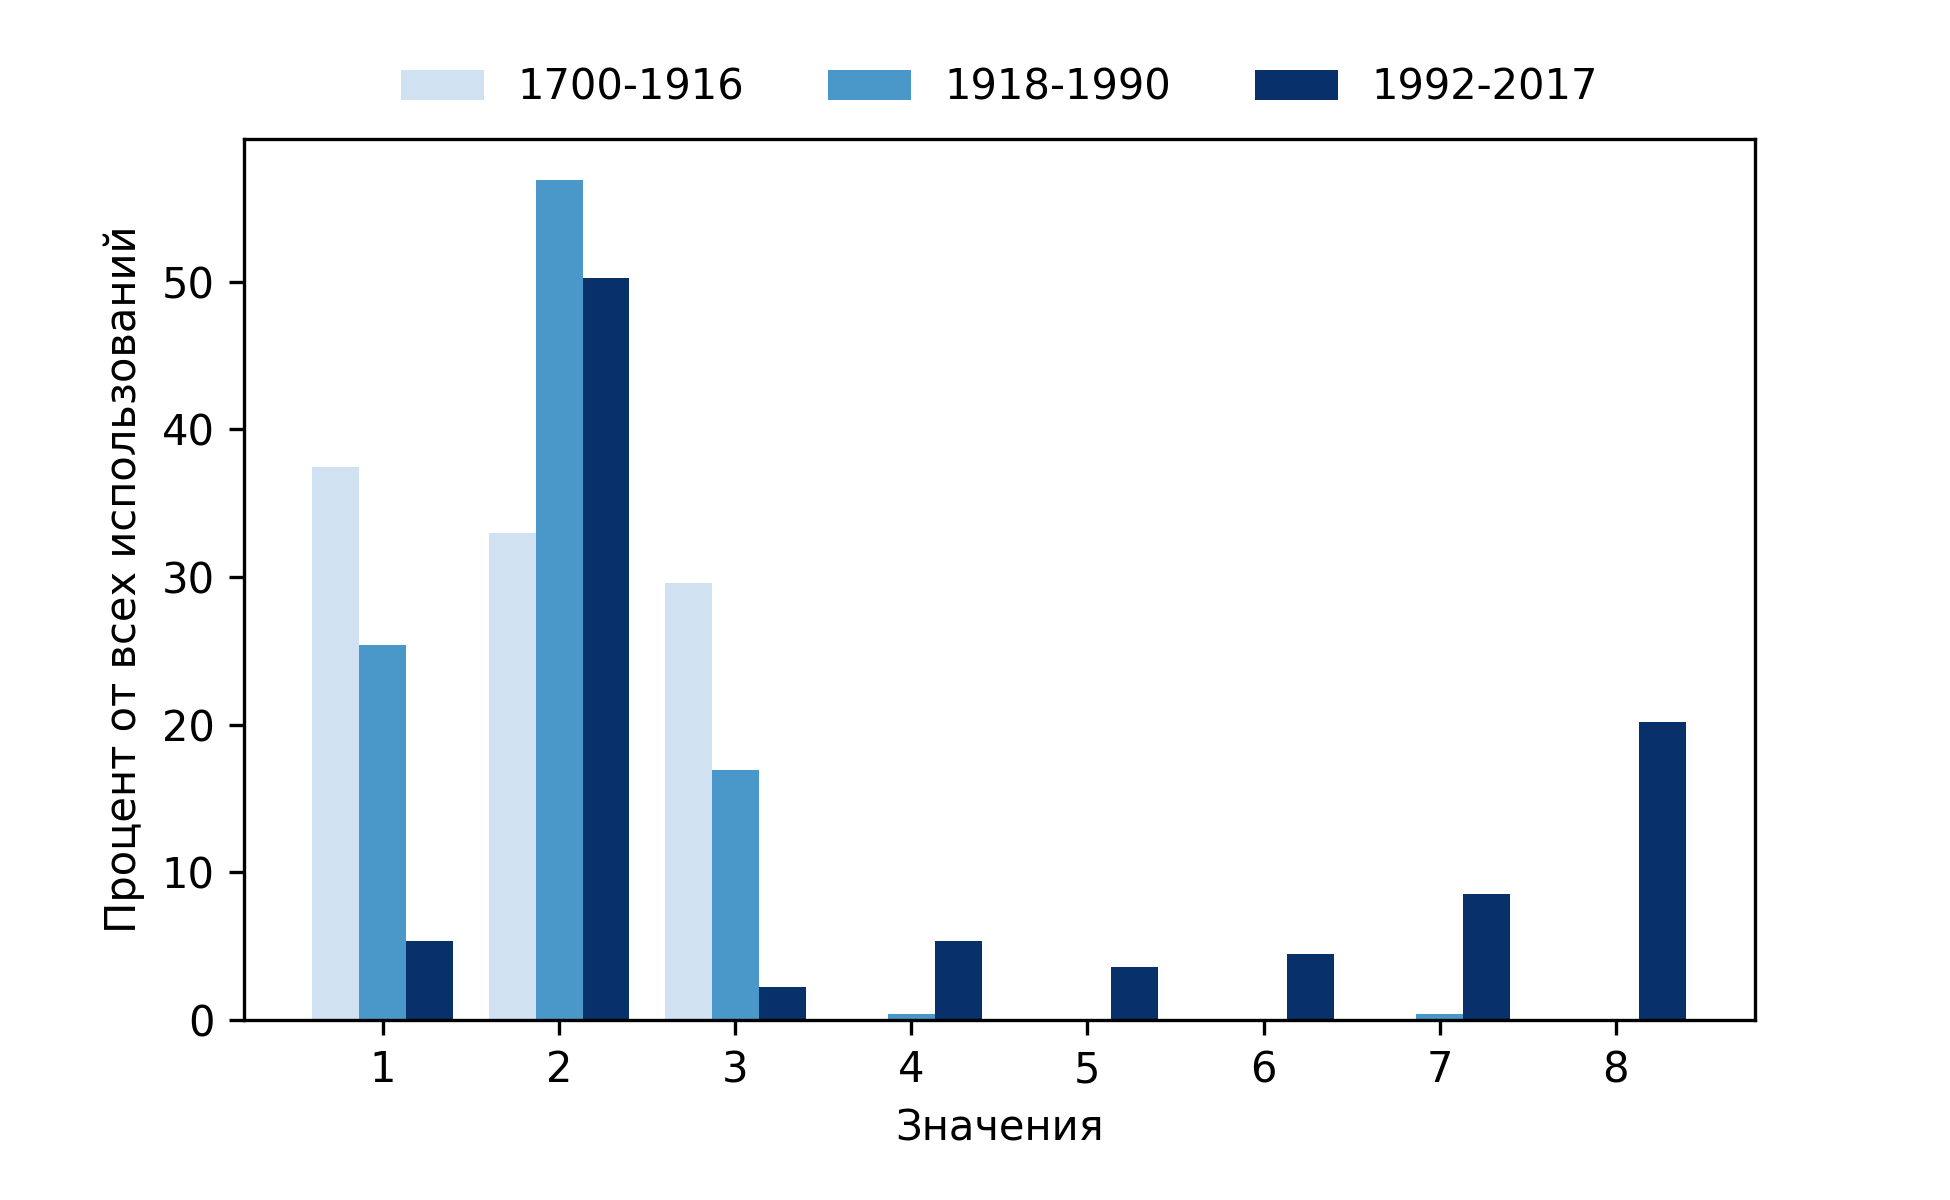
\includegraphics[width=0.8\textwidth]{img/visualizations/paket_minimal}
	\caption{Изменение значений слова \textit{пакет}}
	\label{fig:Пакет}
\end{figure}

Значения для визуализации слова \textit{пакет} (Параметры: eps=0.11, min\_samples=8).

\begin{enumerate}
    \item Письмо, посылка и т. п. в таком виде.
    \item Бумажный или матерчатый мешочек с чем-либо для хранения, перевозки и т. п.
    \item Письмо, посылка и т. п., запечатанные в такой конверт.
    \item Совокупность каких-либо однородных, связанных между собой предметов, явлений и т. п.
    \item Совокупность программных средств, объединенных по какому-либо признаку.
    \item Часть чего-либо, принадлежащая кому-либо на определенных условиях.
    \item Совокупность каких-либо однородных предметов, документов и т. п.
    \item Совокупность акций какого-либо акционерного общества.
\end{enumerate}

\subsubsection*{Анализ значений слова \textit{пакет}}

Все определения, кроме шестого, корректно сформулированы.

\begin{itemize}
    \item ’Письмо, посылка и т. п. в таком виде.’, а также
’Письмо, посылка и т. п., запечатанные в такой конверт.’ имеет общий смысловой элемент с
’Конверт с письмом официально-делового содержания.’, а именно семы \textit{’письмо’}, \textit{’посылка’}, \textit{’конверт’}.

    \item ’Бумажный или матерчатый мешочек с чем-либо для хранения, перевозки и т. п.’ соответствует
’Бумажный или полиэтиленовый мешок для упаковки каких-л. предметов, продуктов и т.п.’,
общие семы \textit{’мешок’}, \textit{’бумажный’}.

    \item ’Совокупность программных средств, объединенных по какому-либо признаку.’ частично соответствует
’Набор взаимосвязанных элементов, объединённых общей целью.’,
так как включает те же семы \textit{’совокупность’}, \textit{’объединенных объектов’},
но является более узким, так как касается только программных средств.
Среди примеров, которые были выделены алгоритмом, находятся такие, как
\textit{Для обработки же растровых изображений и конкретно цифровых фотографий у компании \("\)Corel\("\)
существует пакет Corel Paint Shop Pro Photo.}, где значение слова действительно может
быть описано как ’Совокупность программных средств, объединенных по какому-либо признаку.’,
поэтому мы будем считать это определение корректным.

    \item ’Совокупность акций какого-либо акционерного общества.’ полностью соответствует
’Некоторое число акций какого-либо предприятия или компании, которым владеет человек или какая-либо организация, предприятие.’,
так как включает те же семы \textit{’совокупность’}, \textit{’акции’}.

    \item ’Совокупность каких-либо однородных, связанных между собой предметов, явлений и т. п.’,
, а также ’Совокупность каких-либо однородных предметов, документов и т. п.’
соответствует ’Набор взаимосвязанных элементов, объединённых общей целью.’.  % TODO: посмотреть использования
\end{itemize}

\begin{itemize}
    \item ’Часть чего-либо, принадлежащая кому-либо на определенных условиях.’ не
имеет схожих определений среди обобщенных и является некорректным.
Анализ примеров, для которых алгоритм дал такое определение, показывает, что
большинство примеров связано с акциями, например, \textit{Но контрольный пакет акций был размыт}.
В данном случае логичным является определение, акцентирующее \textit{’совокупность’}.
\end{itemize}

Обобщённые значения, не найденные в визуализации:
\begin{itemize}
    \item ’Упакованный в бумажную или иную обёртку какой-л. предмет (предметы); свёрток.’
отсутствует среди предложенных моделью значений.

    \item ’Стопка ящиков или одинаковых деталей, строительных материалов и т.п.,
уложенных на специальный поддон для погрузки, перевозки и т.п.’
также отсутствует в визуализации.
%Это значение акцентируется на физической стопке предметов (ящиков, деталей) на поддоне,
%что могло быть причиной отсутствия в визуализации.
Можно предположить, что модель могла не выделить это значение из-за ограниченного
количества использований в датасете.
\end{itemize}

Таким образом, для лексемы \textit{пакет} представлено 7 корректных определений.
Среди ошибок присутствуют:
\begin{itemize}
    \item Некорректность определения: 1
\end{itemize}

Перейдем к частотности значений.

Основные изменения в значениях слова \textit{пакет}, указанные в книге «Два века в двадцати словах»,
расположены на Рисунке~\ref{TwoCenturiesPaket}.
В досоветский период значения, обозначающие ’почтовое отправление’ и ’упаковка, свёрток’
уступили место ’мешку, в том числе из полиэтилена’, ’набору’ и ’картонной упаковке’.
Информация из визуализации предложенного подхода частично соответствует этим данным.
’Письмо, посылка и т. п. в таком виде.’ и ’Письмо, посылка и т. п., запечатанные в такой конверт.’
вместе преобладают в досоветский период, уступая место значению
’Бумажный или матерчатый мешочек с чем-либо для хранения, перевозки и т. п.’ в советское время.
Кроме того, согласно алгоритму, в постсоветское время появляются такие значения, как
’Совокупность каких-либо однородных, связанных между собой предметов, явлений и т. п.’,
’Совокупность акций какого-либо акционерного общества.’,
что соответствует информации из книги.

\begin{figure}[H]
    \centering % Centers the images
    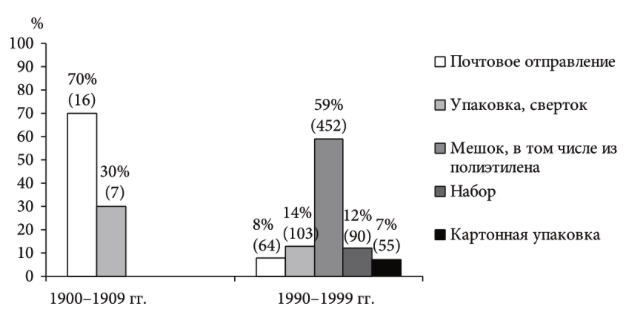
\includegraphics[width=0.8\textwidth]{img/book/paket/1900-1999}
    \caption{Значения слова \textit{пакет} для 1900-1999 согласно~\cite{TwoCenturies}}
    \label{TwoCenturiesPaket}
\end{figure}

Таким образом, предложенный подход в целом отражает значения, в которых использовалось
слово \textit{пакет}, согласуясь с данными из толкового словаря и историческим исследованием.

\section{Результаты качественного анализа}

В результате обобщения словарных дефиниций было составлено 121 значение для 20 слов.

Всего в результате работы предложенного подхода было получено 83 определения для 20 слов. %92

Таким образом, без учёта некорректных определений было успешно выявлено
64.4\% значений.

\begin{table}[H]
\centering
\caption{Типы определения и их количество}
\begin{tabular}{|>{\raggedright\arraybackslash}p{8cm}|c|c|}
\hline
\textbf{Тип определения} & \textbf{Количество} & \textbf{Процент} \\ \hline
Корректные & 57 & 68.67\% \\ \hline %57
Близкие & 10 & 12.04\% \\ \hline %10
Некорректные & 5 & 6.02\% \\ \hline %5
Недостаточно конкретизированные & 3 & 3.61\% \\ \hline %5
Избыточность или чрезмерное использование общих фраз & 4 & 4.81\% \\ \hline
Близкое значение, а также избыточность или чрезмерное использование общих фраз & 1 & 1.20\% \\ \hline
Избыточно конкретизированные & 3 & 3.61\% \\ \hline
Самореференция & 0 & 0.00\% \\ \hline
Противоположное значение & 0 & 0.00\% \\ \hline
Неправильная часть речи & 0 & 0.00\% \\ \hline
\end{tabular}
\end{table}

Как видно, из результатов большинство определений являются корректными
без каких-либо ошибок или недочётов (68.67\%).

Кроме того, проблема с самореференцией была успешно решена.

Из частых проблем можно выделить:
\begin{itemize}
    \item \textbf{Близкое значение.}
Примером можно привести определение ’Насекомое, похожее на червя, а также его личинка.’
для слова \textit{червяк},
где допущена ошибка, так как червь не может быть взрослым насекомым.
Возможно, часть таких ошибок связана с относительно небольшим размером модели,
что не позволяет ей иметь уверенные знания об окружающем мире.

    \item \textbf{Некорректность.}
Примером является ’Употребляется для присоединения предложений или отдельных членов предложений,
усиливающих или уточняющих высказанную мысль.’
для слова \textit{пожалуй}.
Как видно, определение слова \textit{пожалуй} не соответствует его правильному значению,
что также может быть связано с ограничениями модели.

    \item \textbf{Избыточность или чрезмерное использование общих фраз.}
В нашем случае эта проблема проявляется в повторении слов в определении.
Например, для слова \textit{свалка} в сгенерированном определении ’Беспорядочная, беспорядочная схватка.’
повторяется слово \textit{беспорядочная}.
На наш взгляд, именно такая ошибка может быть связана с обилием синонимических рядов в определениях
обучающего датасета на основе «Малого академического словаря»,
что является одним из способов описать значение слова в лексикологии.

    \item \textbf{Недостаточное конкретизирование.}
Например, ’Ласковое обращение к женщине.’ для слова \textit{мама} близко к
’Обращение ребёнка к своей матери.’, но имеет более широкий смысл, включающий всех женщин,
а не только матерей или нянь, что делает его недостаточно специфичным. % TODO: дописать
\end{itemize}

Кроме того, одной из выявленных проблем является недостаток контекста для разграничения значения.
Возьмём как пример слово \textit{пионер}.

Для него новым значением является ’Член добровольной самодеятельной детской организации.’,
появившееся в советское время.
В визуализации указано около 20\% использований слова в таком значении
в досоветский период, что объясняется двусмысленностью части примеров,
например, \textit{Пионеры слушают это и восхищаются.}, где необходим дополнительный контекст
для установления значения.

К сожалению, для 2 слов из списка представляется невозможным полноценно проанализировать
статистическую информацию.
Этими словами являются \textit{публика} и \textit{сволочь}.

Так, для слова \textit{публика} в книге «Два века в двадцати словах» не даётся
диаграмм частотности для слова \textit{публика}.
Говорится лишь о преобладании значения ’аудитория’ и о его оттенках,
которые не удается полноценно сравнить из-за того, что алгоритм предложил довольно общие значения.

Для слова \textit{сволочь} из 4 значений, выявленных при обобщении дефиниций,
предложенным подходом были выявлены только следующие два значения:
\begin{enumerate}
    \item Употребляется как бранное слово.
%    \item Таща, доставить куда-либо.
    \item О подлом, гнусном человеке.
\end{enumerate}

К сожалению, оба выделенных значения подпадают под значение ’Индивидуальное оскорбление.’
в книге «Два века в двадцати словах».
Также в визуализации отсутствуют ключевые значения,
которые часто использовались в досоветский период, такие как ’Собирательное наименование для дрянных, подлых людей; сброд, подонки’.
Таким образом, анализ изменений значения сделать не представляется возможным.

Кроме того, затруднителен анализ для слова \textit{кануть}.
Для него подтверждается информация о том, что с 1900 года ’исчезнуть, сгинуть, пропасть’ является
основным значением, однако книга не предоставляет визуализаций частоты
использования значений слова по периодам.

Среди большинства оставшихся слов визуализации в той или иной степени совпадают с данными из книги «Два века в двадцати словах».
Исключением является рассмотренное ранее слово \textit{пока}, где результаты визуализации противоречат
данным исследования.

Так, основные изменения значения, согласующиеся с данными из книги, были
выявлены в 12 словах – большинстве.

Одна из самых качественных визуализаций была сделана для слова \textit{пакет}.
Так, в нём было выявлено 7 корректных определений,
4 из которых встречаются только в постсоветский период:
\begin{itemize}
    \item Совокупность каких-либо однородных, связанных между собой
предметов, явлений и т. п.
    \item Совокупность программных средств, объединенных по какому-
либо признаку.
    \item Совокупность каких-либо однородных предметов, документов и т.
п.
    \item Совокупность акций какого-либо акционерного общества.
\end{itemize}
2 определения, связанные со значением ’письма’ теряют в популярности в советский и постсоветский период,
а значение ’бумажного или матёрчатого мешочка’ растёт в использовании.

Все вышеперечисленные результаты согласуются с данными из исследования истории данных слов.

Кроме того, в 4 словах изменения были также выявлены и частично согласуются.

Таким образом, представляется возможным утверждать, что моделирование определений даёт
интерпретируемые описания значений слов, которые могут быть успешно использованы
для выявления семантических изменений.

%Обобщёнными для него являлись значения:
%\begin{enumerate}
%    \item В течение некоторого времени; до сих пор ещё; впредь до чего-л.
%    \item В то время как.
%    \item До того времени как.
%    \item Употребляется при прощании, до свидания.
%\end{enumerate}
%
%Алгоритмом были сформулированы следующие значения:
%\begin{enumerate}
%    \item В настоящее время, до тех пор.
%    \item Употребляется при обозначении времени, в течение которого совершается действие.
%    \item Употребляется при прощании с кем-л.
%\end{enumerate}
%
%\begin{figure}[H]
%	\centering
%	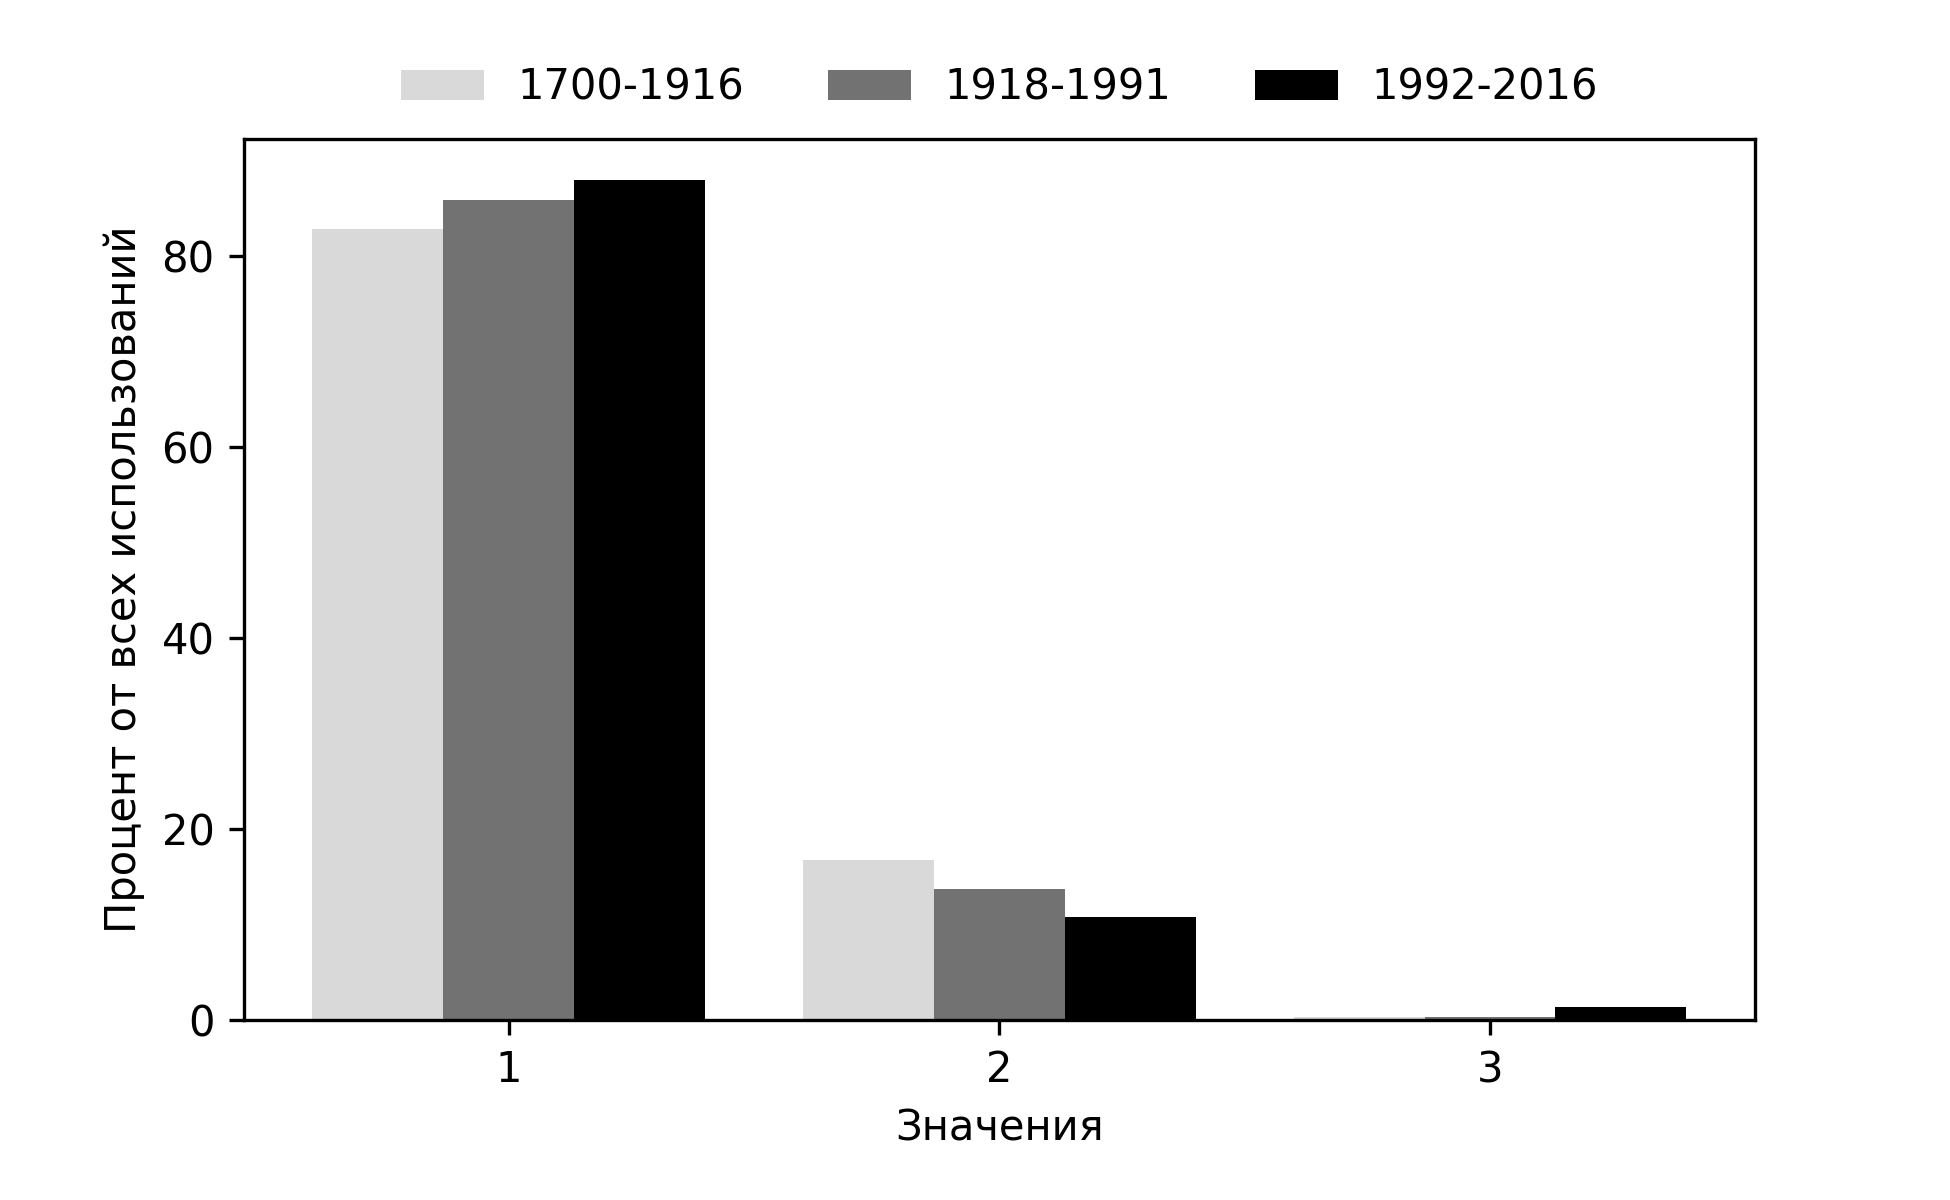
\includegraphics[width=0.8\textwidth]{img/visualizations/poka_minimal}
%	\caption{Изменение значений слова \textit{пока}}
%	\label{fig:Пока_2}
%\end{figure}
%
%В книге сообщается, что изначальным и всегда преобладающим было использование слова в качестве
%союза, после чего в XIX веке появилось использование как наречие, а затем в советский период
%– как этикетное слово.
%Данные из визуализации алгоритма (график снизу) поддерживают появление значения
%’Употребляется при прощании с кем-л.’
%поздно – несколько процентов для постсоветского периода, однако данные для наречия и союза
%не совпадают.
%Можно предположить, что модели сложно различать эти значения из-за их схожести.
%Например, для
%«Когда мы забирали щенка, нас предупредили, что ей категорически нельзя наверх забираться,
%пока у нее слабые лапы.»
%было сгенерировано ’В настоящее время, до тех пор.’,
%что относит его к наречию,
%но из примера видно, что пока связывает части предложения и является союзом.

%\begin{figure}[H]
%    \centering % Centers the images
%    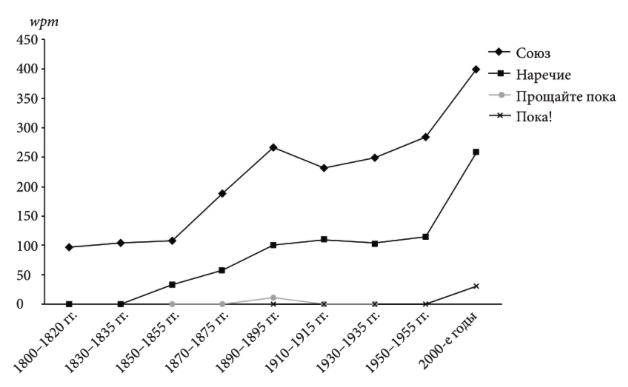
\includegraphics[width=0.8\textwidth]{img/book/poka/all}
%    \caption{Значения слова \textit{пока} согласно~\cite{TwoCenturies}}
%\end{figure}

\subsection*{Выводы}

Таким образом, была дообучена большая языковая модель FRED-T5-1.7B для задачи
генерации определений с помощью датасета на основе «Малого академического словаря».
Проведенные эксперименты показали,
что модель способна генерировать семантически близкие,
но не всегда идентичные определения.
Несмотря на сравнительно низкие значения метрик BLEU и ROUGE-L,
отражающих формальное сходство сгенерированных определений с эталонными,
модель демонстрирует высокие результаты по метрике BERT-F1,
учитывающей семантическую близость текстов.
Это говорит о том, что модель способна генерировать определения,
имеющие схожий смысл с эталонными, хоть и зачастую сформулированные иными словами.

Применение модели для анализа семантических сдвигов на материале соревнования Rushifteval показало,
что решение на основе FRED-T5-1.7B вместе с дообучением векторизатора способно добиться высокого
результата в лидерборде.
Таким образом, данная модель демонстрирует хорошие результаты в задаче выявления семантических изменений.

Разработанная визуализация на основе кластеризации векторных представлений определений позволяет
наглядно представить семантические изменения слов во времени,
что может быть полезно для исследований в лексикологии и истории языка.

Кроме того, была произведена качественная оценка работы модели на примере произведённых
с её помощью визуализаций, в ходе которого было определено, что большинство
из сгенерированных определений являлись корректными, а статистическая информация
по изменению использования отдельных значений во времени преимущественно совпадала
с результатами экспертного исследования истории слов.

\chapter*{Заключение}

Таким образом, в ходе выполнения выпускной квалификационной работы была обучена генеративная языковая модель
на основе материала словаря МАС для задачи генерации определений слов на основе их
контекста использования.
Кроме того, были выполнены следующие задачи:
\begin{itemize}
    \item разработан алгоритм автоматического определения семантических сдвигов на
основе векторного представления сгенерированных определений,
    \item проведён анализ метрик и качества обученной языковой модели и
сравнение её с существующими аналогами,
    \item был разработан алгоритм визуализации результатов,
    \item проведён качественный анализ результатов предложенного подхода.
\end{itemize}

Модель показала высокие результаты метрики сходства BERTScore для тестовой выборки,
а также успешно показала себя на тестовом материале Rushifteval,
имея результаты сопоставимые с лидирующими решениями.
При качественном анализе результатов предложенный подход показал высокие результаты, выявив большинство значений,
а также верно составив визуализацию изменения использования значений для большинства слов.
В процессе выполнения настоящей работы было доказано, что моделирование определений может быть
успешно применено для задачи детектирования семантических изменений,
а также позволяет достичь высокого уровня интерпретируемости.

%В ходе выполнения выпускной квалификационной работы была обучена генеративная языковая модель
%на основе архитектуры Трансформер для задачи генерации определений слов на основе их
%контекста использования.
%Модель показала высокие результаты метрики сходства BERTScore для тестовой выборки,
%а также успешно показала себя на тестовом материале Rushifteval,
%имея результаты сопоставимые с лидирующими решениями.
%Кроме того, был создан алгоритм визуализации результатов модели,
%благодаря которому наше решение имеет высокую степень интерпретируемости.
%после чего был произведен качественный анализ работы алгоритма.
%В нем алгоритм показал высокие результаты, выявив большинство значений,
%а также верно составив визуализацию изменения использования значений для большинства слов.
%В целом, выполнения настоящей работы было доказано, что моделирование определений может быть
%успешно применено для задачи детектирования семантических изменений.

Результаты настоящей работы можно применять для определения степени семантического сдвига лексем
с наличием визуализации и определений для каждого выявленного значения,
что может быть использовано в лексикологии,
где необходимы актуальные данные для построения новых словарей~\cite{DefinitionGenerationMainArticle}.
Кроме того, модель, позволяющая автоматически генерировать качественные словарные определения,
может быть полезна в таких задачах обработки естественного языка,
как анализ тональности, машинный перевод и разграничение семантической
неоднозначности~\cite{DefinitionModelingReviewAndDatasetAnalysis}.

Перспективами развития настоящего исследования является:
\begin{itemize}
    \item Использование более одного словаря в качестве материала для обучения модели,
    \item Использование генеративных моделей большего размера, чем используется в работе.
\end{itemize}

Полученные результаты имеют высокую научную ценность,
предложенный подход имеет ряд преимуществ по сравнению с существующими аналогами.
Созданные программные модули для обучения,
визуализации и оценки качества нейросетевых алгоритмов могут быть внедрены в профильные прикладные системы.

%Ограничениями подхода можно считать необходимость в значительных вычислительных ресурсах.
%Несмотря на то, что FRED-T5-1.7B запускается на ЦПУ, запуск на большом количестве вхождений
%займет значительное число времени.
%Для запуска на ГПУ же необходима видеокарта с 8 ГБ видеопамяти.
%
%Код, использованный во время выполнения настоящей работы, выложен в открытый доступ
%на сайте GitHub и может быть воспроизведен.~\citeurl{WorkGitHub}

\printbibliography
\appendix
\chapter{Качественный анализ}

\section*{Знатный}

В результате анализа семем лексемы \textit{знатный} в толковых словарях были выделены пять групп значений,
которые можно сформулировать следующим образом:

\begin{enumerate}
    \item Известный, знаменитый, прославленный своей деятельностью. \textit{Знатная бетонщица Савелова!}
    (\textit{«Известный, знаменитый, прославленный.»} в БТС,
    \textit{«Прославившийся своей деятельностью, такой, к-рого знают все.»} в ТСО,
    \textit{«Выдающийся в труде.»} в «Двух веках в двадцати словах»)

    \item Принадлежащий к знати, к аристократии, к верхушке привилегированного класса. \textit{Знатный род.}
    (\textit{«Принадлежащий к знати, к верхушке привилегированного класса.»} в БТС,
    \textit{«Принадлежащий к аристократии, к знати.»} в ТСО,
    \textit{«Принадлежащий к знати, высокий по чину.»} в «Двух веках в двадцати словах»)

    \item Отличный, высокий по качеству. \textit{Знатный табак.}
    (\textit{«Отличный, высокий по качеству; сильный.»} в БТС,
    \textit{«Отличный, высокий по качеству; сильный (прост.).»} в ТСО,
    \textit{«Хороший.»} в «Двух веках в двадцати словах»)

    \item Существенный, серьезный (усилитель). \textit{Была знатная акция.}
    (\textit{«Существенный, серьезный (усилитель).»} в «Двух веках в двадцати словах»)

    \item Знаемый, известный, видимый. \textit{Знатен волк.}
    (\textit{«Знаемый, известный, видимый.»} в «Двух веках в двадцати словах»)
\end{enumerate}

\begin{figure}[H]
	\centering
	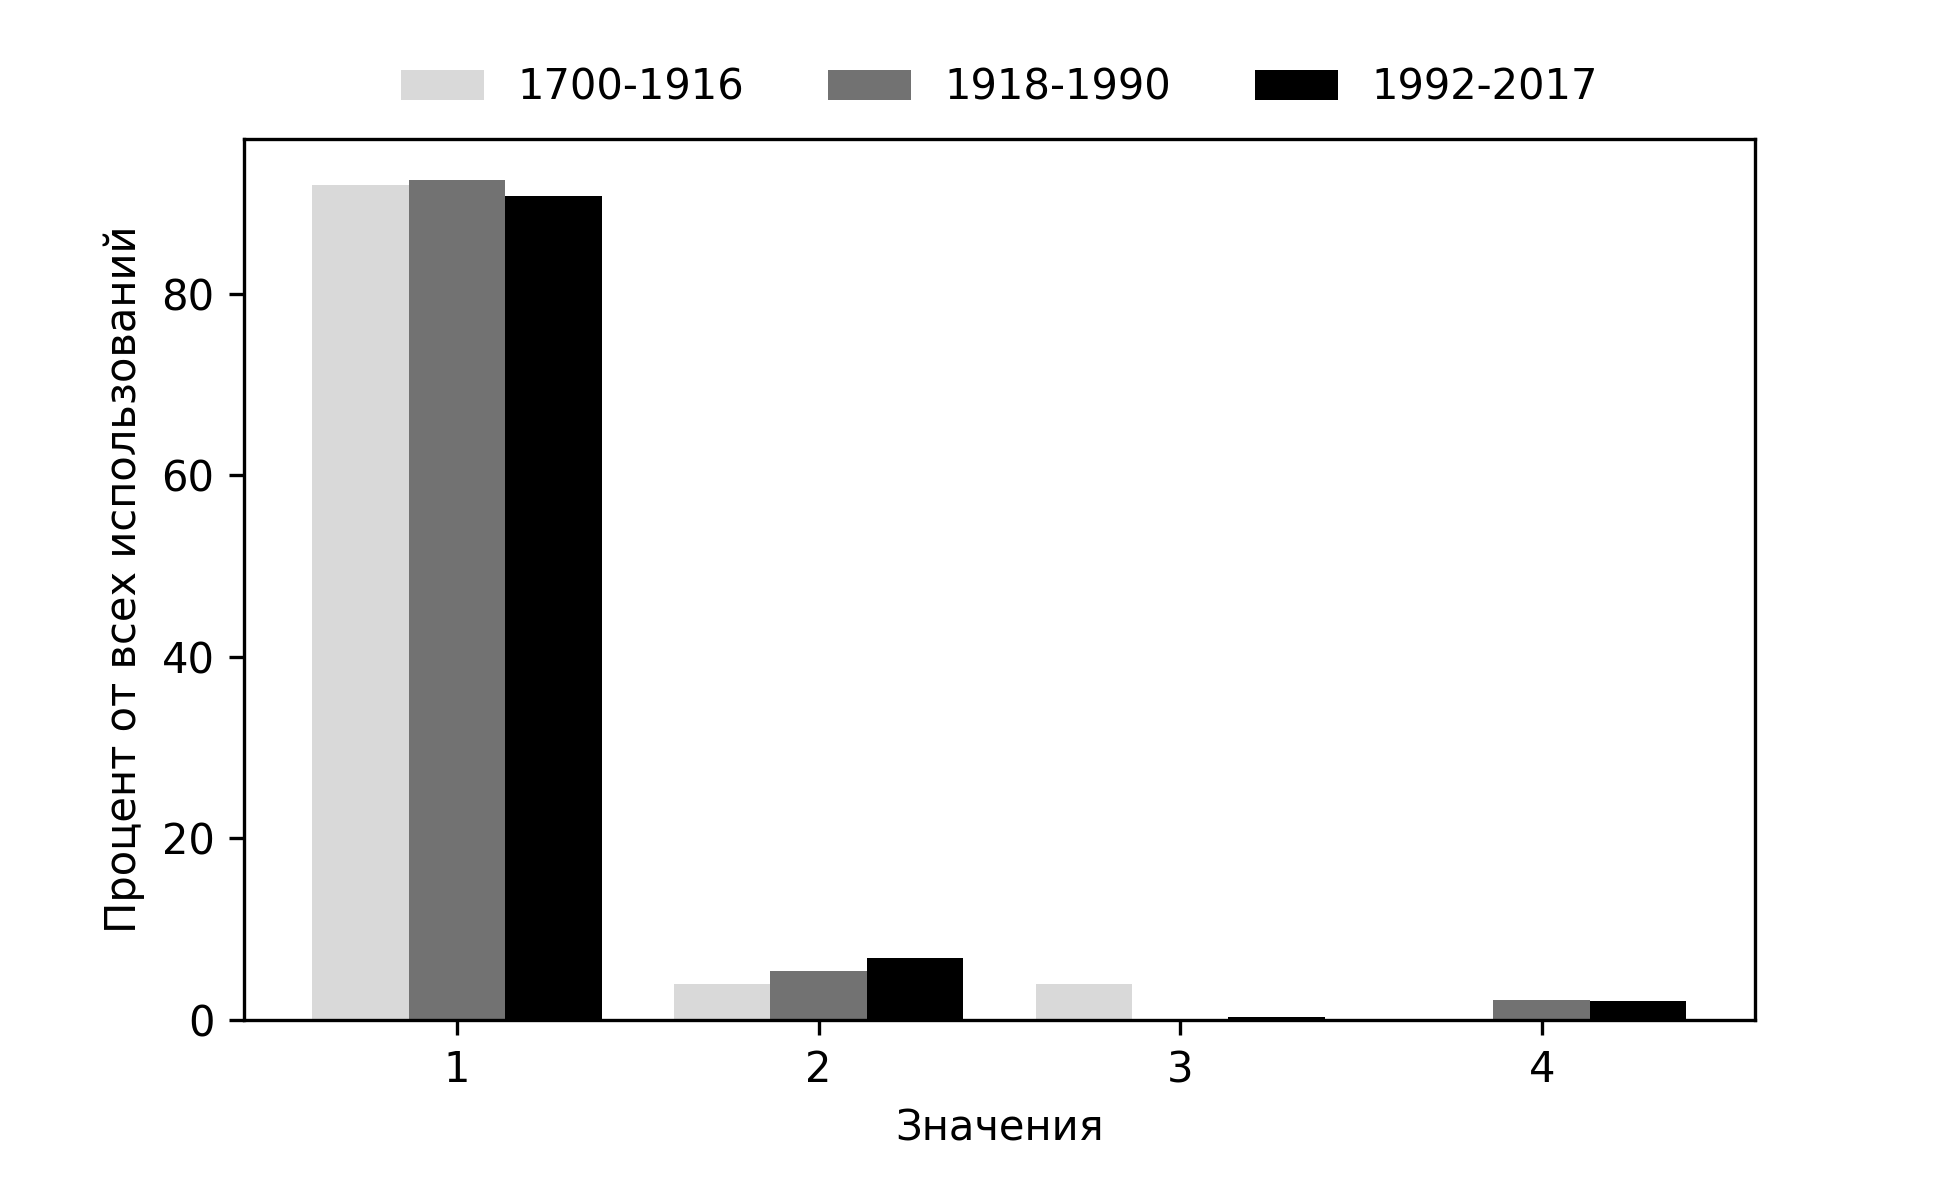
\includegraphics[width=0.8\textwidth]{img/visualizations/znatnyj_minimal}
	\caption{Изменение значений слова \textit{знатный}}
	\label{fig:Знатный}
\end{figure}

Значения для визуализации слова \textit{знатный} (Параметры: eps=0.15, min\_samples=10).

\begin{enumerate}
    \item Принадлежащий к знати, имеющий высокое общественное положение.
    \item Очень хороший, превосходный.
    \item Значительный по значению, важный, значительный.
    \item Знающий свое дело, искусный, опытный.
\end{enumerate}

\subsection*{Анализ значений слова \textit{знатный}}

Первое и второе определения корректно сформулированы.
Третье и четвертое определения соответствуют обобщенным значениям.
Пятое определение не соответствует обобщенным значениям.

\begin{itemize}
    \item ’Принадлежащий к знати, имеющий высокое общественное положение.’ имеет общий смысловой элемент с
’Принадлежащий к знати, к аристократии, к верхушке привилегированного класса.’,
а именно семы \textit{’принадлежность к знати’}, \textit{’высокое общественное положение’}.

    \item ’Очень хороший, превосходный.’ полностью соответствует ’Отличный, высокий по качеству.’,
так как включает те же семы \textit{’отличный’}, \textit{’высокий по качеству’}, \textit{vпревосходный’}.

    \item ’Значительный по значению, важный, значительный.’ соответствует
’Существенный, серьезный (усилитель).’, так как включает те же семы \textit{’важность’}, \textit{’серьезность’}.

    \item ’Знающий свое дело, искусный, опытный.’ частично соответствует
’Известный, знаменитый, прославленный своей деятельностью.’,
%так как включает семы \textit{’искусный’}, \textit{’опытный’}, которые подразумевают известность и признание в своей деятельности.
так как включает семы \textit{’искусный’}, \textit{’опытный’}, которые подразумевают профессионализм работника в своей области.
\end{itemize}

Обобщённые значения, не найденные в визуализации:
\begin{itemize}
    \item ’Знаемый, известный, видимый’ также отсутствует в визуализации.
Это значение могло быть не выделено из-за недостаточной частотности.
\end{itemize}

Таким образом, для лексемы \textit{знатный} представлено 3 корректных определения.
Среди ошибок присутствуют:
\begin{itemize}
    \item Близкие: 1
\end{itemize}

Перейдем к частотности значений.

Информация из «Двух веков в двадцати значениях» представлена на графиках~\ref{fig:TwoCentruriesZnatniy1} и~\ref{fig:TwoCentruriesZnatniy2}
В книге можно выделить три основных момента.
Во-первых, наличие до конца XVIII века значения ’Знаемый, известный, видимый’,
однако оно не было выделено алгоритмом.
Во-вторых, преимущественное использование значения
’Принадлежащий к знати, имеющий высокое общественное положение.’ на протяжении
всего исследуемого времени.
Такой же результат наблюдается и в визуализации, с 90\% использования на протяжении трех эпох.
В-третьих, появление в советский период значения, связанного с трудом,
что так же отражается на построенном графике.

\noindent % Prevents indentation for this line to align the images at the left margin
\begin{figure}[H]
    \centering % Centers the images
    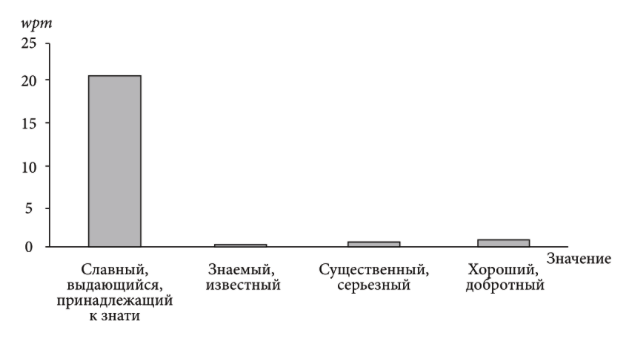
\includegraphics[width=0.8\textwidth]{img/book/znatnij/1891-1920}
    \caption{Значения слова \textit{Знатный} для 1891-1920 согласно~\cite{TwoCenturies}}
    \label{fig:TwoCentruriesZnatniy1}
\end{figure}

%\begin{figure}[H]
%    \centering % Centers the images
%    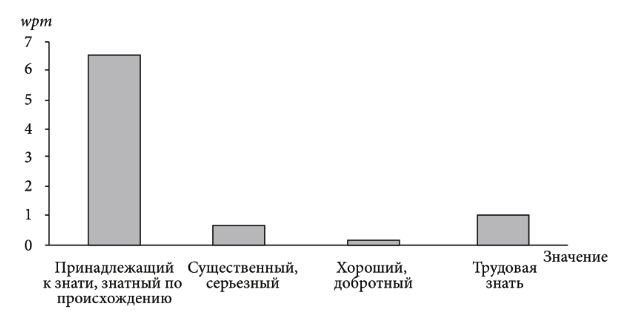
\includegraphics[width=0.8\textwidth]{img/book/znatnij/1921-1950}
%    \caption{Second Image Caption}
%\end{figure}

\begin{figure}[H]
    \centering % Centers the images
    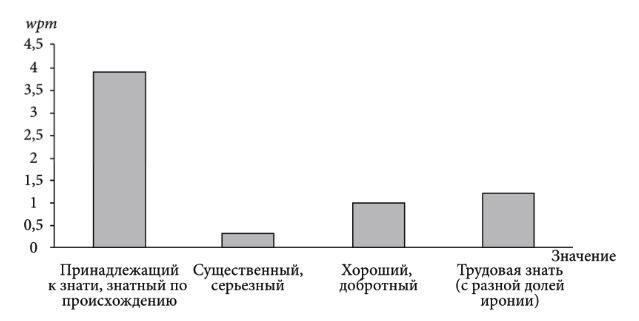
\includegraphics[width=0.8\textwidth]{img/book/znatnij/1990-2010}
    \caption{Значения слова \textit{Знатный} для 1990-2010 согласно~\cite{TwoCenturies}}
    \label{fig:TwoCentruriesZnatniy2}
\end{figure}

Таким образом, алгоритм в целом отражает значения, в которых использовалось
слово \textit{знатный}, согласуясь с данными из толкового словаря и историческим исследованием.
Алгоритм выделяет как основное значение, связанное с высоким положением, так и большинство
менее частых.

\section*{Кануть}

В результате анализа семем лексемы \textit{кануть} в толковых словарях были выделены пять групп значений,
которые можно условно сформулировать следующим образом:

\begin{enumerate}
    \item Упасть каплей; капнуть. \textit{Канула слеза.}
    (\textit{«Упасть каплей; капнуть.»} в БТС,
    \textit{«Капнуть, упасть каплей (устар.).»} в ТСО,
    \textit{«Капнуть.»} в «Двух веках в двадцати словах»)

    \item Погрузиться, утонуть. \textit{Канул на дно реки.}
    (\textit{«Упав куда-л., во что-л., погрузиться.»} в БТС,
    \textit{«Утонуть, упасть на дно.»} в «Двух веках в двадцати словах»)

    \item Бесследно исчезнуть, пропасть. \textit{Куда же он канул?}
    (\textit{«Пропасть, исчезнуть, скрыться.»} в БТС,
    \textit{«Бесследно пропасть, исчезнуть.»} в ТСО,
    \textit{«Пройти, минуть, исчезнуть.»} в «Двух веках в двадцати словах»)

    \item Пройти, миновать. \textit{Та жизнь уже канула?}
    (\textit{«Пройти, минуть, исчезнуть.»} в «Двух веках в двадцати словах»)

    \item Исчезнуть из виду. \textit{А потом канет дорога в сосняк.}
    (\textit{«Исчезнуть из виду.»} в «Двух веках в двадцати словах»)
\end{enumerate}

%Выражения (фразеологизмы):
%\begin{itemize}
%    \item Кануть в Лету. Быть забытым, бесследно исчезнуть.
%    (\textit{«Кануть в Лету (быть забытым, бесследно исчезнуть).»} в БТС,
%    \textit{«Кануть в Лету (бесследно исчезнуть из памяти людей; высок.; в греческой мифологии Лета — река забвения).»} в ТСО)
%
%    \item Как (будто, словно) в воду канул. Исчезнуть, пропасть бесследно.
%    (\textit{«Как (будто, словно) в воду канул. Исчез, пропал бесследно.»} в БТС,
%    \textit{«Как в воду канул кто бесследно исчез.»} в ТСО)
%\end{itemize}

\begin{figure}[H]
	\centering
	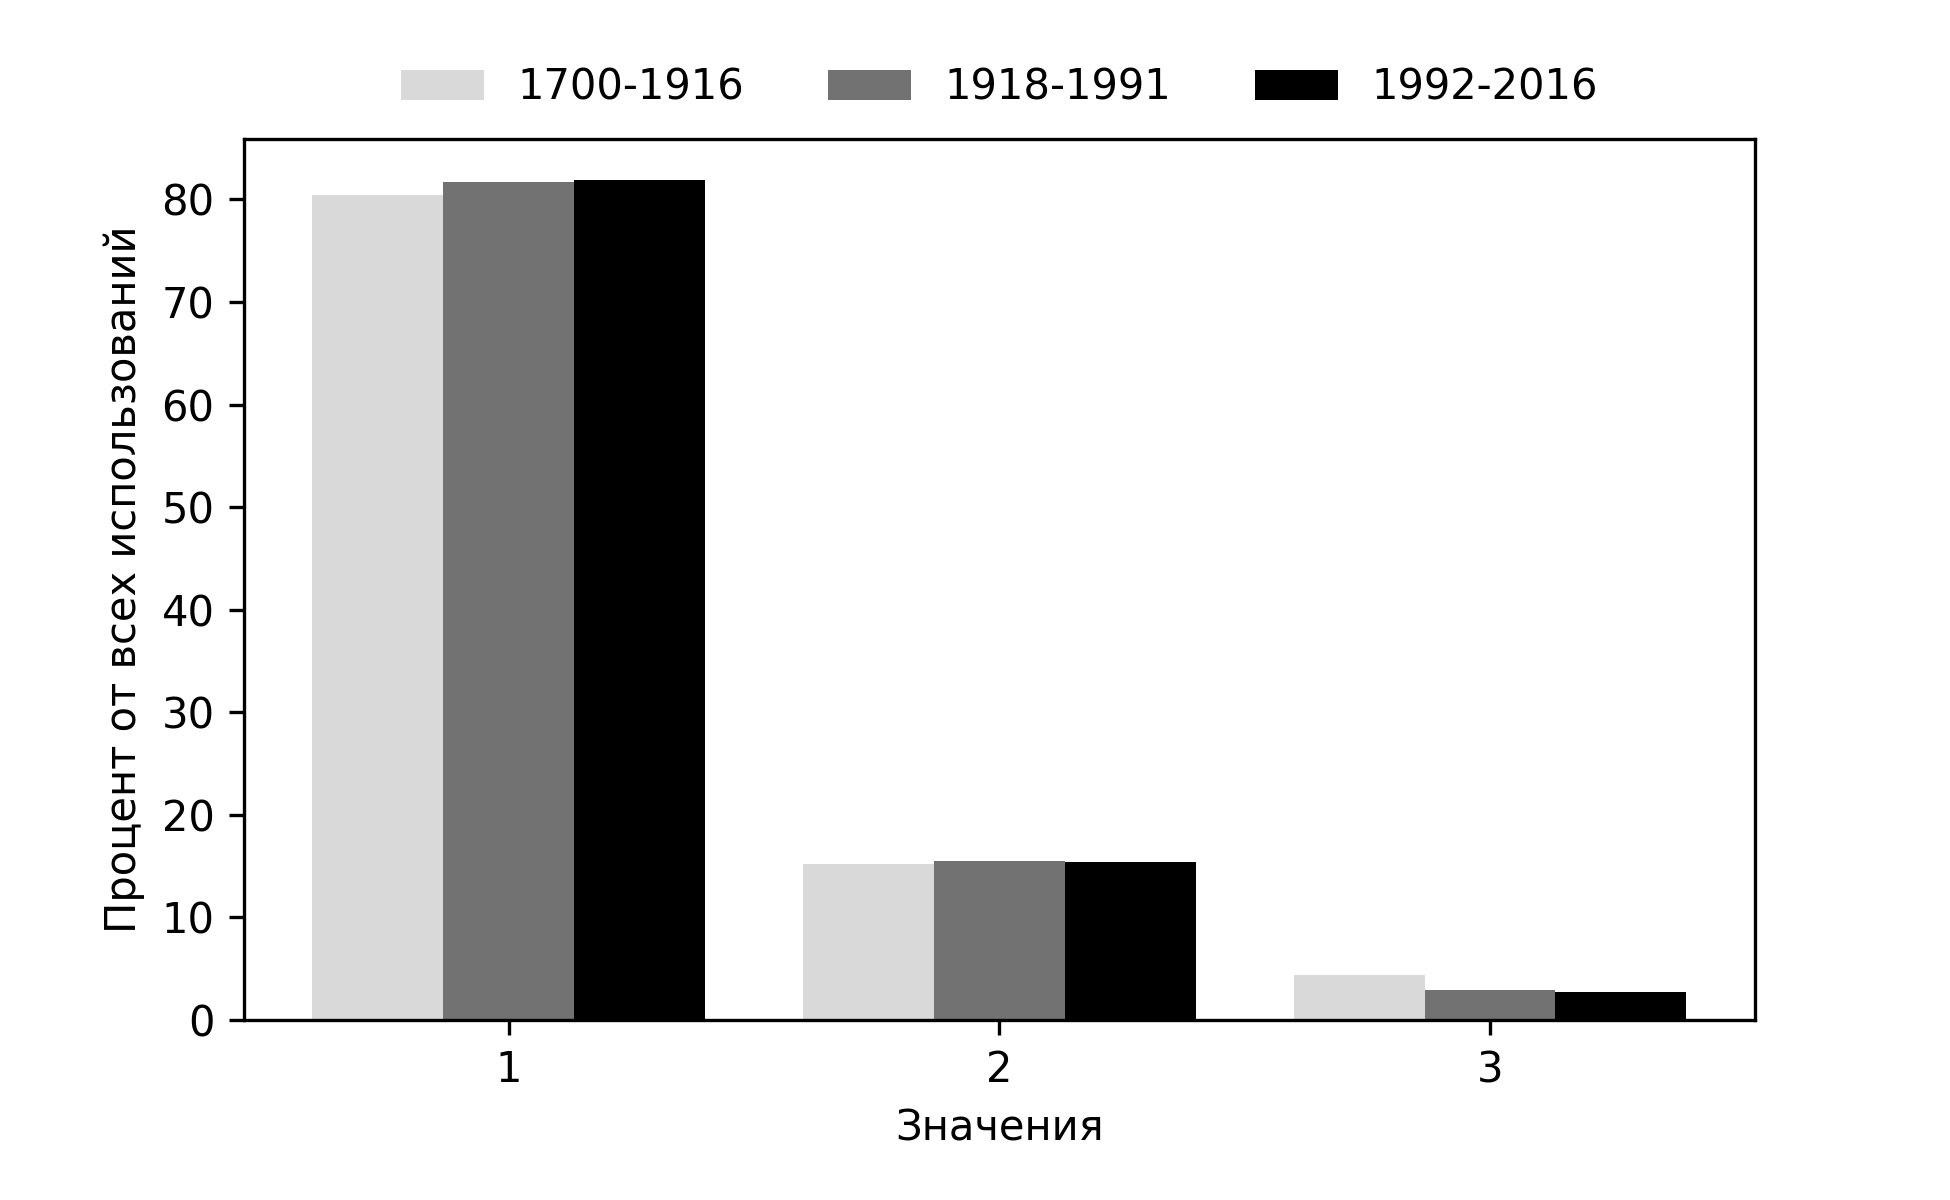
\includegraphics[width=0.8\textwidth]{img/visualizations/kanut'_minimal}
	\caption{Изменение значений слова \textit{кануть}}
	\label{fig:Кануть}
\end{figure}

Значения для визуализации слова \textit{кануть} (Параметры: eps=0.18, min\_samples=10).

\begin{enumerate}
    \item Исчезнуть, пропасть.
    \item Пройти, миновать, исчезнуть.
    \item Упасть, погрузиться.
\end{enumerate}

\subsection*{Анализ значений слова \textit{кануть}}

Первые три определения корректно сформулированы.

\begin{itemize}
    \item ’Исчезнуть, пропасть.’ корректное определение, так как имеет общий смысловой элемент с
’Бесследно исчезнуть, пропасть.’, а именно семы \textit{’исчезнуть’} и \textit{’пропасть’}.

    \item ’Пройти, миновать, исчезнуть.’ соответствует
’Пройти, миновать.’, так как включает те же семы \textit{пройти’}, \textit{миновать’}.
%Визуализация добавляет сему \textit{’миновать’}, что расширяет значение, делая его более широким.

    \item ’Упасть, погрузиться.’ частично соответствует ’Погрузиться, утонуть.’,
так как включает семы \textit{’упасть’} и \textit{’погрузиться’}.
\end{itemize}

\begin{itemize}
    \item ’Упасть каплей; капнуть.’ не выделяется алгоритмом.
Можно предположить, что это значение недостаточно часто встречается.
В «Двух веках в двадцати словах» указано, что на протяжении XIX века оно заменяется
другими значениями.
\end{itemize}

Таким образом, для лексемы \textit{кануть} представлено 2 корректных определения.
Среди ошибок присутствуют:
\begin{itemize}
    \item Близкие значения: 1
\end{itemize}

Перейдем к частотности значений.

Затруднительно провести анализ рассматриваемого слова,
так как, судя по «Двум векам в двадцати словах» выделенные алгоритмом значения появляются
в досоветский период и продолжают использоваться дальше.
Подтверждается информация о том, что с 1900 года ’исчезнуть, сгинуть, пропасть’ является
основным значением слова, однако книга не предоставляет визуализаций частоты
использования значений слова по периодам.

\section*{Классный}

В результате анализа семем лексемы \textit{классный} в толковых словарях были выделены пять групп значений,
которые можно условно сформулировать следующим образом:

\begin{enumerate}
    \item Имеющий отношение к школьному обучению. \textit{Классная доска.}
(\textit{«к Класс (3 зн.)»} в БТС,
\textit{«Классным называют то, что имеет отношению к классу.»} в ТСД,
\textit{«Имеющий отношение к школьному обучению.»} в «Двух веках в двадцати словах»)

    \item Имеющий определённый класс, разряд, соответствующий требованиям такого класса, разряда. \textit{Классы морских судов.}
(\textit{«Имеющий определённый класс, разряд, соответствующий требованиям такого класса, разряда.»} в БТС,
\textit{«Имеющий класс (разряд).»} в «Двух веках в двадцати словах»)

    \item Имеющий определённый ранг, чин. \textit{Небольшой классный чиновник.}
(\textit{«Имеющий определённый ранг, чин.»} в БТС,
\textit{«Классный чиновник.»} в «Двух веках в двадцати словах»)

    \item Специалист, обладающий высоким мастерством в своей области. \textit{Классный водитель.}
(\textit{«Принадлежащий к высшему классу, разряду по квалификации, по мастерству в чём-л.»} в БТС,
\textit{«Классным называют специалиста, который обладает высоким мастерством в своей области.»} в ТСД)

    \item Отличный, высокого качества. \textit{Обед был классный!}
(\textit{«Отличный.»} в БТС,
\textit{«Принадлежащий к высшему классу (в 4 знач.), высокого качества (разг.).»} в ТСО,
\textit{«Классным называют человека, предмет, событие и т. п., которые имеют замечательные свойства,
обладают высоким качеством; разговорный стиль.»} в ТСД,
\textit{«Хороший, отличный.»} в «Двух веках в двадцати словах»)
\end{enumerate}

\begin{figure}[H]
	\centering
	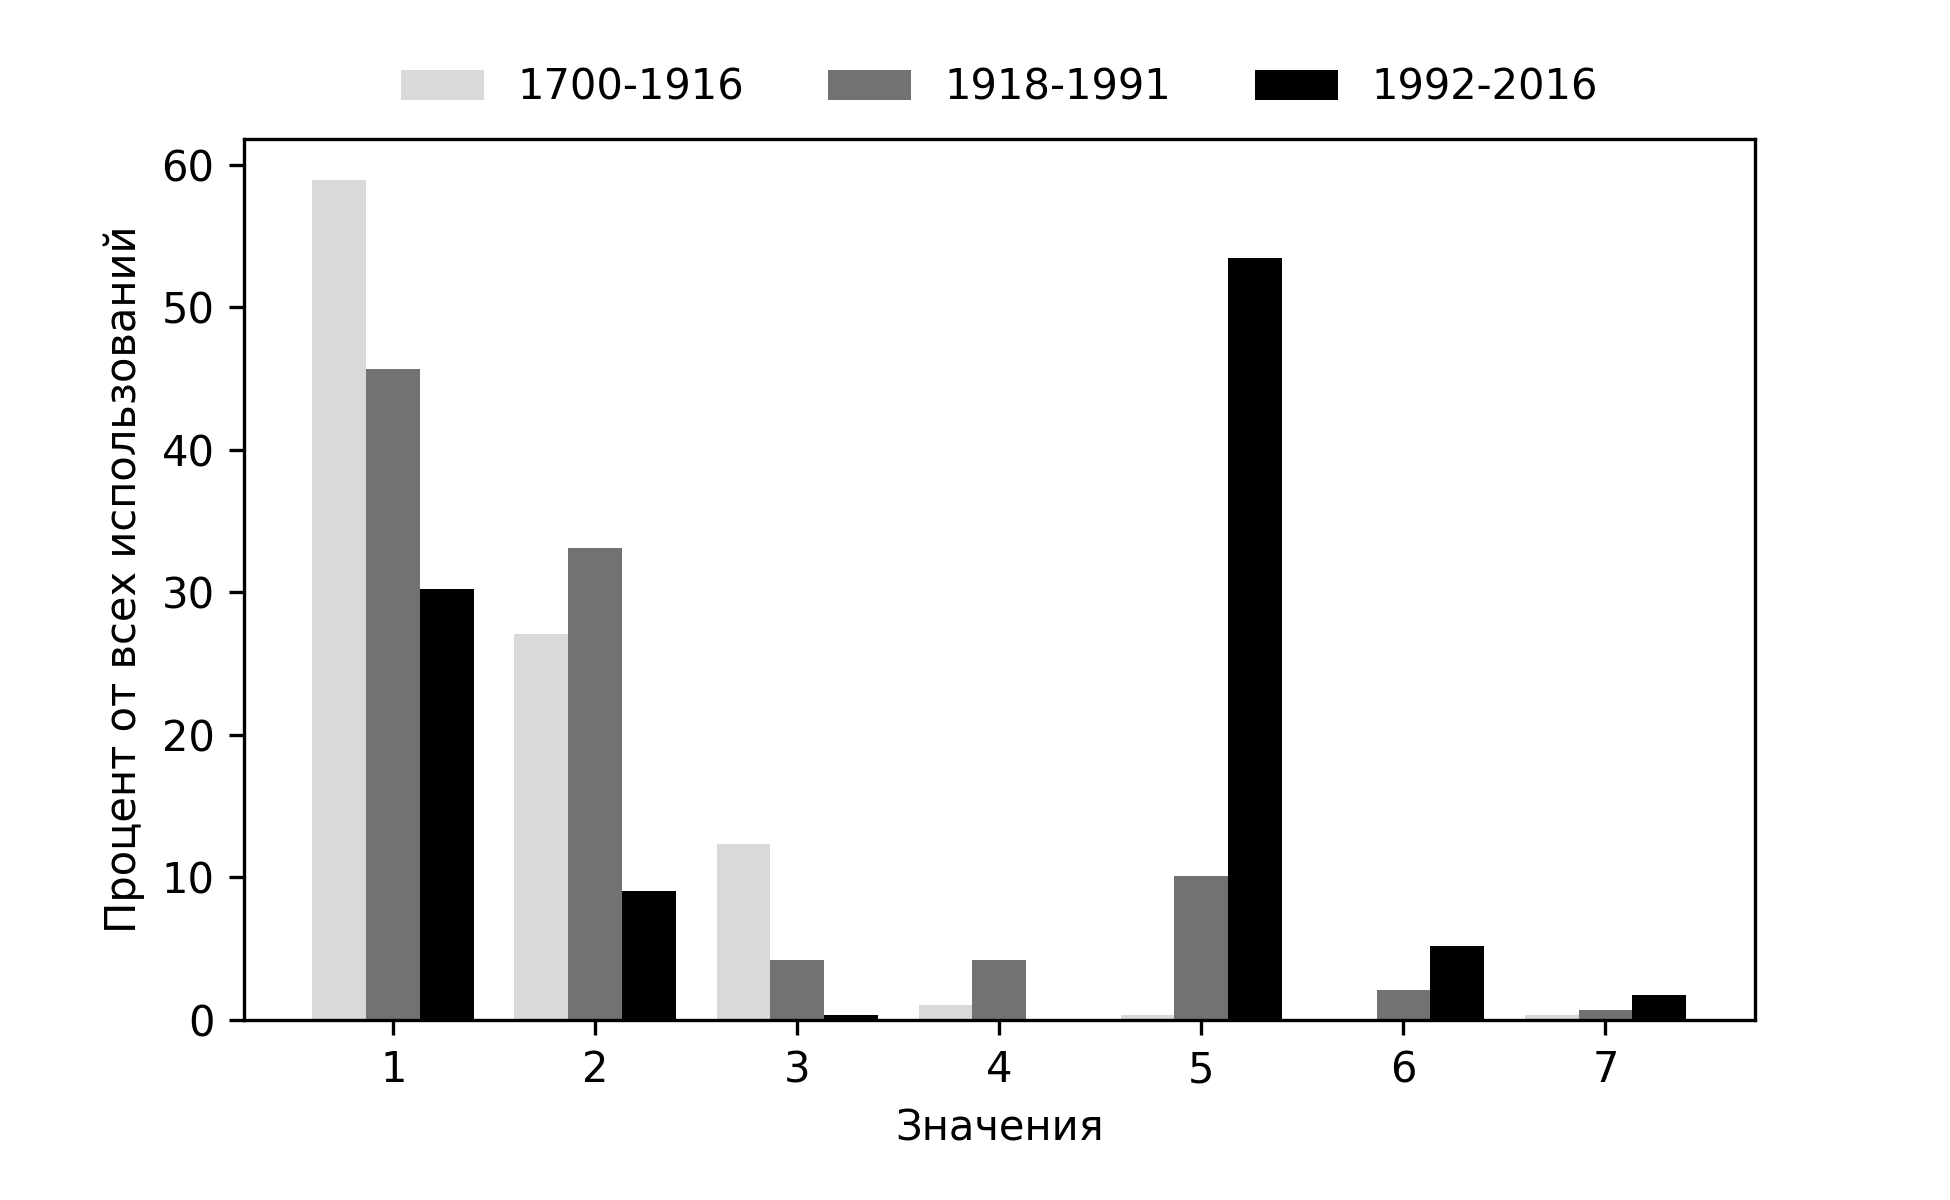
\includegraphics[width=0.8\textwidth]{img/visualizations/klassnyj_minimal}
	\caption{Изменение значений слова \textit{классный}}
	\label{fig:Классный}
\end{figure}

Значения для визуализации слова \textit{классный} (Параметры: eps=0.22, min\_samples=5).

\begin{enumerate}
    \item Служащий в классе, занимающийся в классе.
    \item Предназначенный для класса.
    \item Помещение для занятий в школе.
    \item Предназначенный для пассажиров первого класса.
    \item Очень хороший, замечательный.
    \item Отличающийся высоким мастерством в каком-л. деле.
    \item Связанный с присвоением какого-либо звания, чина.
\end{enumerate}

\subsection*{Анализ значений слова \textit{классный}}

Третье и четвертое определения не соответствуют обобщенным значениям.
Остальные определения являются корректными.

\begin{itemize}
    \item ’Служащий в классе, занимающийся в классе.’ соответствует определению
’Имеющий отношение к школьному обучению.’, объединяя семы \textit{’служащий’}, \textit{’занимающийся’}, \textit{’класс’}.

    \item ’Предназначенный для класса.’ также относится к определению
’Имеющий отношение к школьному обучению.’ с теми же семами.

    \item ’Очень хороший, замечательный.’ соответствует значению ’Отличный, высокого качества.’,
объединяя семы \textit{’хороший’}, \textit{’отличный’}, \textit{’высокого качества’}.

    \item ’Отличающийся высоким мастерством в каком-л. деле.’ соответствует значению
’Специалист, обладающий высоким мастерством в своей области.’,
объединяя семы \textit{’высокий мастерство’}, \textit{’специалист’}, \textit{’область’}.

    \item ’Связанный с присвоением какого-либо звания, чина.’ аналогично определению
’Имеющий определённый ранг, чин.’, объединяя семы \textit{’звание’}, \textit{’чин’}, \textit{’ранг’}.
\end{itemize}

Слишком специфичные значения:
\begin{itemize}
    \item ’Помещение для занятий в школе.’ является избыточно конкретизированным
и может быть включено в ’Имеющий отношение к школьному обучению.’

    \item ’Предназначенный для пассажиров первого класса.’ также является избыточно конкретизированным,
может быть включено в ’Имеющий определённый класс, разряд, соответствующий требованиям такого класса, разряда.’.
\end{itemize}

Таким образом, для лексемы \textit{классный} представлено 5 корректных определений.
Среди ошибок присутствуют:
\begin{itemize}
    \item Избыточное конкретизирование: 2
\end{itemize}

Перейдем к частотности значений.

Основными моментами из книги «Два века в двадцати словах» является появление
в советское время значения ’Очень хороший, замечательный.’,
становление его основным в постсоветский период и
преобладание значений, связанных со школой, до этого.
Всё вышеперечисленное выводится из нашей визуализации,
где значение ’Очень хороший, замечательный.’ набирает около 10\% от всех
использований в советский период и около 55\% в постсоветский.
Значения, связанные со школьным обучением (1, 2, 3) вместе набирают
более 90\% от всех использований в досоветский период.
Информация из книги «Два века в двадцати словах» приведена в графике~\ref{fig:TwoCenturiesKlassnij}.

\begin{figure}[H]
    \centering % Centers the images
    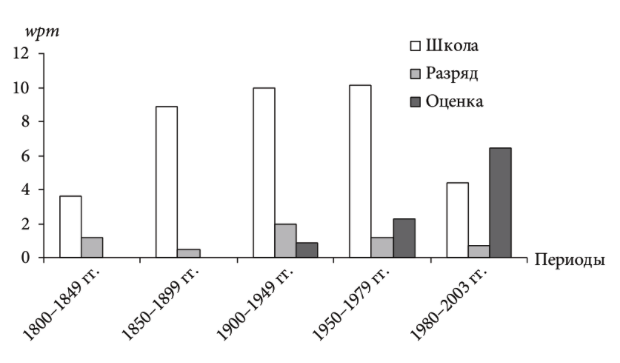
\includegraphics[width=0.8\textwidth]{img/book/klassnij/all}
    \caption{Значения слова \textit{Классный} согласно~\cite{TwoCenturies}}
    \label{fig:TwoCenturiesKlassnij}
\end{figure}

Таким образом, алгоритм отражает значения, в которых использовалось
слово \textit{классный}, согласуясь с данными из толкового словаря и историческим исследованием,
однако некоторые определения являются слишком специфичными.

\section*{Мама}

В результате анализа семем лексемы \textit{мама} в толковых словарях были выделены
пять групп значений, которые можно условно сформулировать следующим образом:

\begin{enumerate}
    \item Женщина, являющаяся родительницей ребёнка. \textit{Родная мама.}
(\textit{«Женщина по отношению к своим детям»} в ТСО,
\textit{«Женщина по отношению к рождённым ею детям»} в БТС и ТСД,
\textit{«Генетическая мать»} в «Двух веках в двадцати словах»)

    \item Обращение ребёнка к своей матери. \textit{Мам, дай поесть.}
(\textit{«Мамой ребёнок называет свою мать»} в ТСД,
\textit{«Мама — это обращение ребёнка к своей матери»} в ТСД)

    \item Обращение к тёще или свекрови. \textit{Мама приехала в гости.}
(\textit{«Тёща или свекровь (обычно в семейном обращении)»} в БТС,
\textit{«Мамой в разговорной речи иногда называют тёщу или свекровь»} в ТСД)

    \item Обращение к опекуну или кормильцу без родственных связей. \textit{Мамы не прикармливали пряниками тихонько, а дядьки не дирали за уши за все про все.}
(\textit{«Комилица, няня»} в «Двух веках в двадцати словах»)

    \item Наименование компонента компьютера – материнской платы. \textit{Покупка же новой «мамы» вместе с процессором тянет на 200 долларов.}
(\textit{«Материнская плата»} в «Двух веках в двадцати словах»)
\end{enumerate}

\begin{figure}[H]
	\centering
	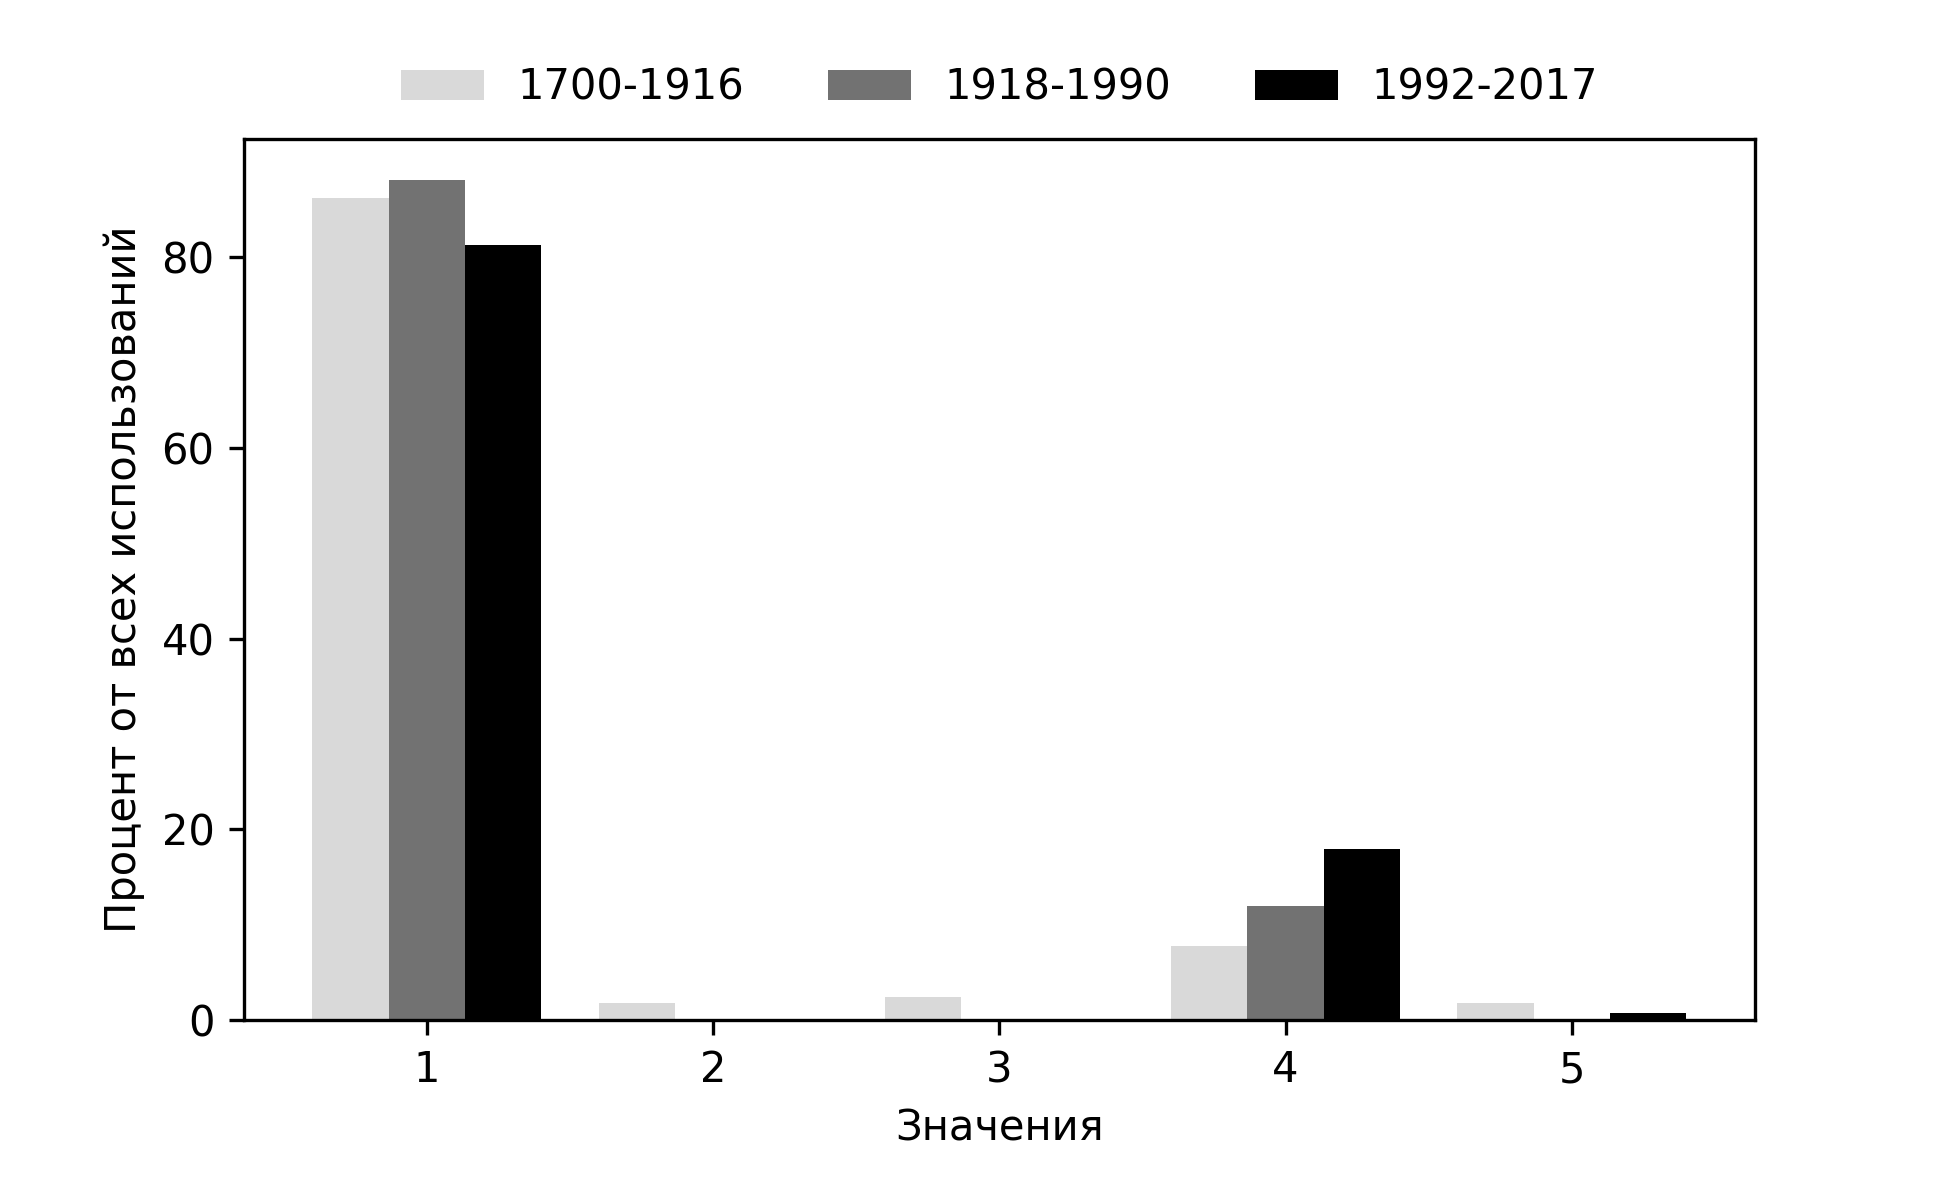
\includegraphics[width=0.8\textwidth]{img/visualizations/mama_minimal}
	\caption{Изменение значений слова \textit{мама}}
	\label{fig:Мама}
\end{figure}

Значения для визуализации слова \textit{мама} (Параметры: eps=0.08, min\_samples=5).

\begin{enumerate}
    \item Женщина, мать.
    \item Фамильярное обращение к пожилому мужчине.
    \item В дореволюционной России: женщина, занимавшаяся воспитанием детей.
    \item Женщина по отношению к своим детям.
    \item Ласковое обращение к женщине.
\end{enumerate}

\subsection*{Анализ значений слова \textit{мама}}

Первое, третье и четвертое определения корректно сформулированы.
Второе и пятое определения не соответствуют обобщенным значениям.

\begin{itemize}
    \item ’Женщина, мать.’ имеет общий смысловой элемент с
’Женщина, являющаяся родительницей ребёнка.’, а именно семы \textit{’женщина’} и \textit{’родитель’}.

    \item ’Женщина по отношению к своим детям.’ полностью соответствует
’Женщина, являющаяся родительницей ребёнка.’, так как включает те же семы \textit{’женщина’}, \textit{’родитель’}.

    \item ’В дореволюционной России: женщина, занимавшаяся воспитанием детей.’ имеет соответствие с
’Обращение к опекуну или кормильцу без родственных связей.’,
так как семы \textit{’женщина’}, \textit{’занимающаяся воспитанием детей’} отражают смысл ’няня’.
\end{itemize}

\begin{itemize}
    \item ’Фамильярное обращение к пожилому мужчине.’ является некорректным значением,
в обобщенных значениях нет упоминаний о мужчине.

    \item ’Ласковое обращение к женщине.’ близко к
’Обращение ребёнка к своей матери.’, но имеет более широкий смысл, включающий всех женщин,
а не только матерей или нянь, что делает его недостаточно специфичным.
\end{itemize}

Обобщённые значения, не найденные в визуализации:
\begin{itemize}
    \item ’Обращение к тёще или свекрови’ отсутствует среди предложенных моделью значений.
Можно предположить, что информации из контекста использований недостаточно для отделения
этого значения от ’женщина, мать.’.

    \item ’Наименование компонента компьютера – материнской платы’ также отсутствует в визуализации.
%Однако, модель способна на выделение данного значения.  % TODO: прогнать на примере модель
\end{itemize}

Таким образом, для лексемы \textit{мама} представлено 3 корректных определения:
Среди ошибок присутствуют:
\begin{itemize}
    \item Некорректность определения: 1
    \item Недостаточное конкретизирование: 1
\end{itemize}

Перейдем к частотности значений.

Основным моментом в Двух веках в двадцати словах для слова \textit{мама}
является появление значения ’Женщина, являющаяся родительницей ребёнка.’, сменивашего
’Обращение к опекуну или кормильцу без родственных связей.’ в середине XIX века.
Это отражено в визуализации алгоритма, где ’В дореволюционной России: женщина, занимавшаяся воспитанием детей.’
присутствует только для досоветского периода.
Основным значением для остальных периодов является ’Женщина, являющаяся родительницей ребёнка.’,
что также отражено в визуализации алгоритма.
Информация из книги приведена в графике~\ref{fig:TwoCenturiesMom}.
Также в книге упоминается появление значения ’Наименование компонента компьютера – материнской платы’
в конце XX века, однако он не был выделен алгоритмом.

\begin{figure}[H]
    \centering % Centers the images
    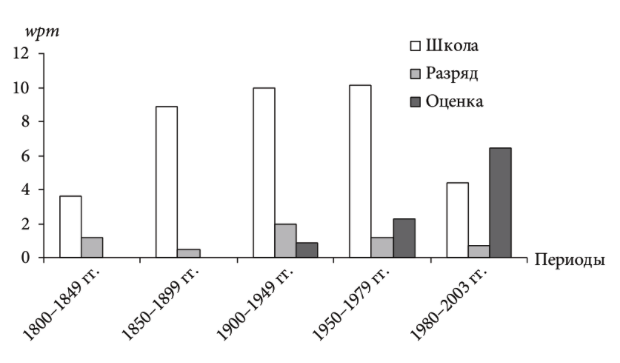
\includegraphics[width=0.8\textwidth]{img/book/klassnij/all}
    \caption{Значения слова \textit{Мама} для 1760-1889 согласно~\cite{TwoCenturies}}
    \label{fig:TwoCenturiesMom}
\end{figure}

Таким образом, алгоритм отражает часть значений, в которых использовалось
слово \textit{мама}, согласуясь с данными из толкового словаря и историческим исследованием.
Часть значений предложена некорректно, так как в них упоминается употребление слова по отношению
к мужчинам, а также по отношению к абсолютно всем женщинам.

\section*{Анализ слова \textit{машина}}

В результате анализа семем лексемы \textit{машина} в толковых словарях были выделены девять групп значений,
которые можно условно сформулировать следующим образом:

\begin{enumerate}
    \item Механическое устройство, совершающее полезную работу с преобразованием энергии, материалов или информации. \textit{Вязальная машина.}
(\textit{«Механизм или совокупность механизмов, совершающие какую-л. полезную работу путём преобразования одного вида энергии в другой.»} в БТС,
\textit{«Механическое устройство, совершающее полезную работу с преобразованием энергии, материалов или информации.»} в ТСО,
\textit{«Машина — это механизм, который совершает какую-либо полезную работу.»} в ТСД,
\textit{«Бытовой прибор»} в «Двух веках в двадцати словах»)

    \item Автомобиль, средство передвижения. \textit{Спортивная гоночная машина.}
(\textit{«Автомобиль, автомашина.»} в БТС,
\textit{«То же, что автомобиль.»} в ТСО,
\textit{«Машина — это средство передвижения, автомобиль.»} в ТСД,
\textit{«Автомобиль»} в «Двух веках в двадцати словах»)

    \item Организация, действующая подобно механизму, налаженно, чётко, бесперебойно. \textit{Военная машина.}
(\textit{«О какой-л. организации, ведомстве и т.п., действующих, подобно механизму, бесперебойно, точно, ритмично.»} в БТС,
\textit{«Об организации, действующей подобно механизму, налаженно и чётко.»} в ТСО,
\textit{«Машиной называют политическую, военную и т. п. организации, которые действуют точно и бесперебойно, как механизм.»} в ТСД)

    \item Человек, лишённый каких-либо эмоций, действующий машинально, автоматически. \textit{Не человек, а машина.}
(\textit{«О человеке, лишённом каких-л. эмоций, действующем машинально, автоматически.»} в БТС,
\textit{«Машиной в разговорной речи называют человека, который никак не проявляет своих чувств, эмоций и совершает поступки машинально, автоматически.»} в ТСД)

    \item Количество груза, вмещающееся в кузов грузового автомобиля. \textit{Привести машину дров.}
(\textit{«О количестве груза, вмещающегося в кузов грузового автомобиля (обычно от 3 до 5 тонн).»} в БТС,
\textit{«Машиной чего-либо в разговорной речи называют количество груза, которое помещается в одну машину.»} в ТСД)

    \item Движущийся или летающий механизм. \textit{Машины с дистанционным управлением.}
(\textit{«О самодвижущихся механизмах различного значения (комбайне, тракторе, мотоцикле и т.п.).»} в БТС,
\textit{«Машиной называют любой движущийся, летающий механизм.»} в ТСД)

    \item Устройство для работы с информацией, компьютер. \textit{Электронно-вычислительная машина.}
(\textit{«Комплекс технических, аппаратных и программных средств, предназначенных для автоматического сбора, хранения, обработки, передачи информации и её использования.»} в БТС,
\textit{«Компьютер.»} в «Двух веках в двадцати словах»)

    \item Мотоцикл, велосипед. \textit{Выбрать машину, которая лучше всего подходит для трассы.}
(\textit{«У спортсменов: мотоцикл, велосипед.»} в ТСО)

    \item Поезд, паровоз. \textit{Стоявшие по сторонам дороги зрители изумлялись, видя величественное, ровное, легкое, притом скорое движение машины.}
(\textit{«Поезд, паровоз.»} в «Двух веках в двадцати словах»)
\end{enumerate}

\begin{figure}[H]
	\centering
	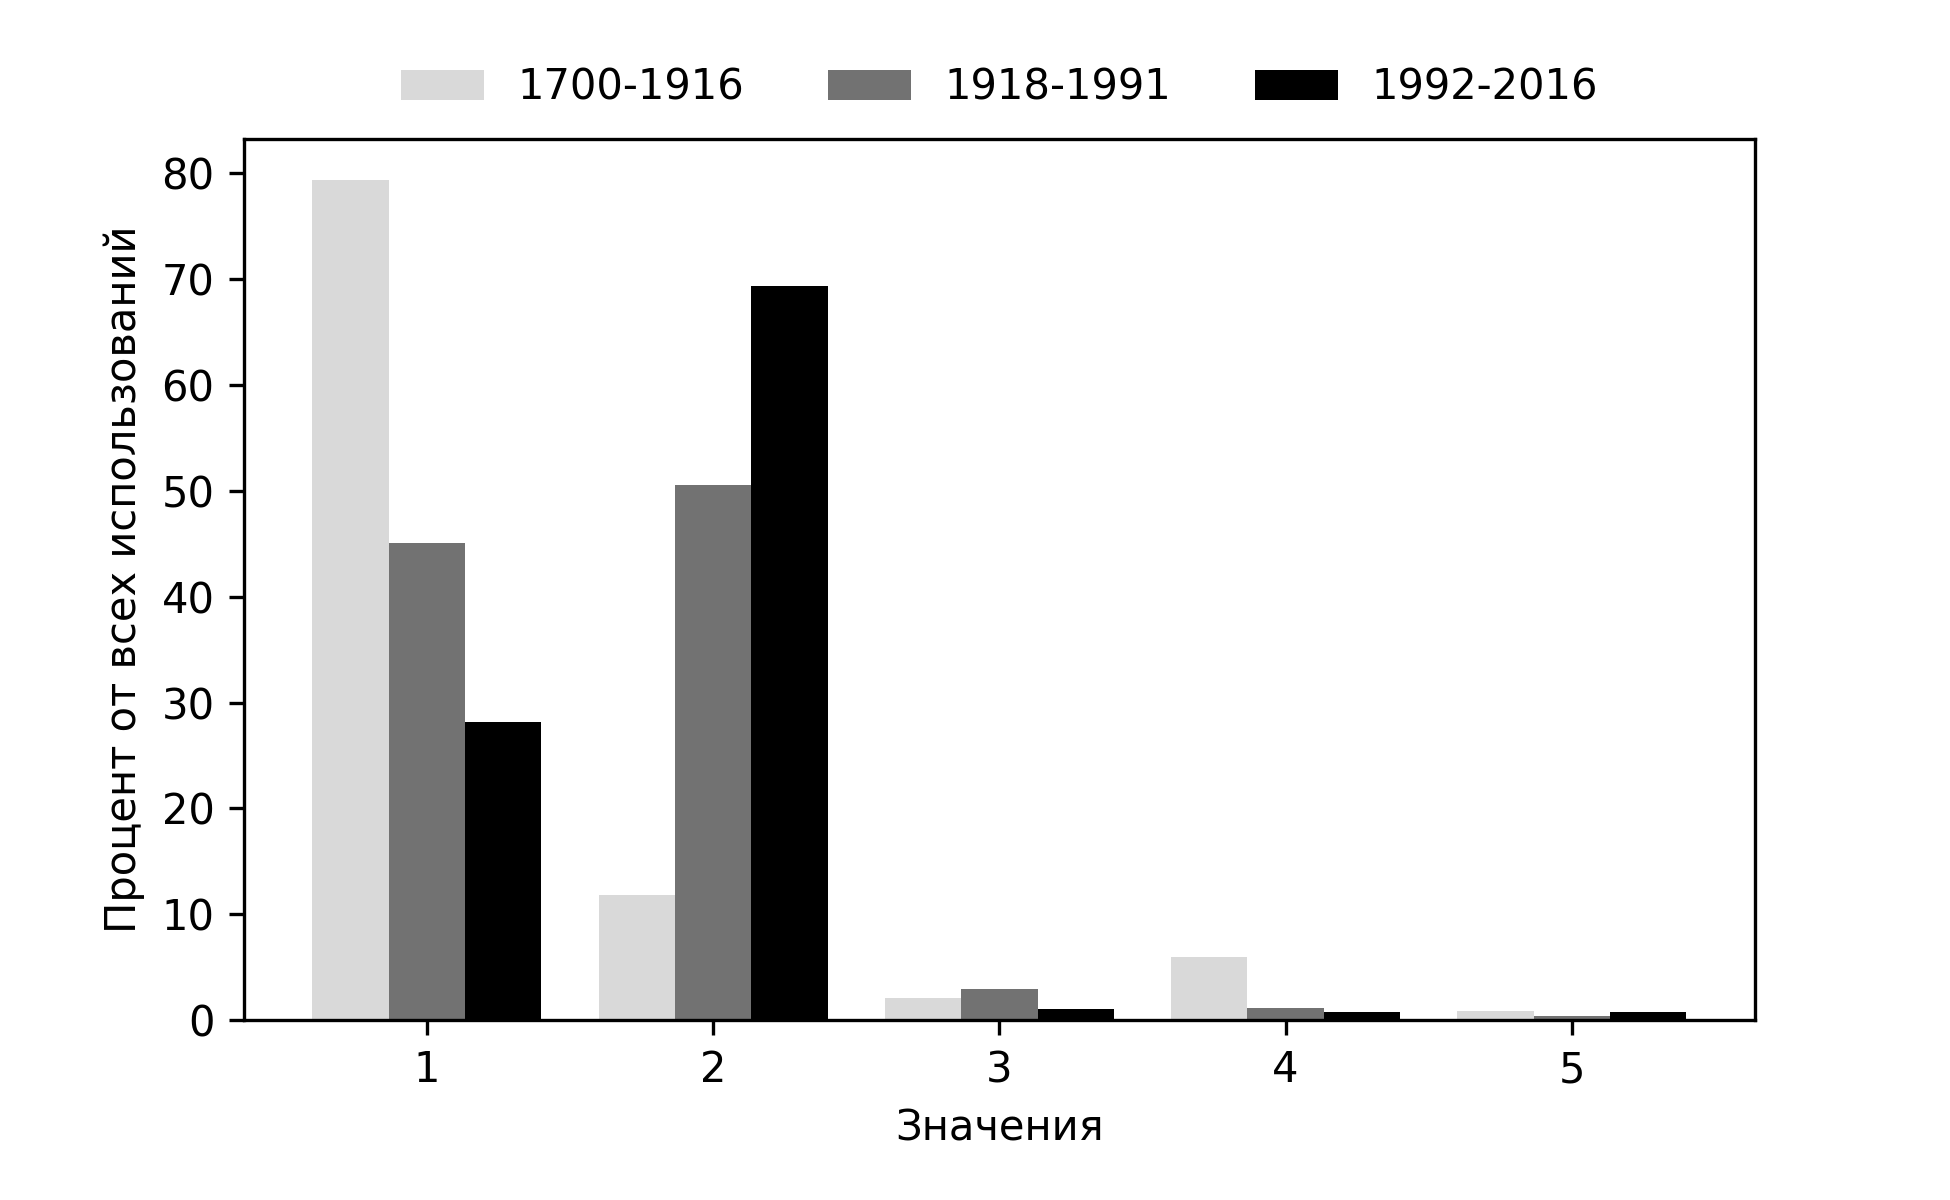
\includegraphics[width=0.8\textwidth]{img/visualizations/mashina_minimal}
	\caption{Изменение значений слова \textit{машина}}
	\label{fig:Машина}
\end{figure}

Значения для визуализации слова \textit{машина} (Параметры: eps=0.14, min\_samples=5).

\begin{enumerate}
    \item Приспособление, устройство, служащее для выполнения какой-л. работы.
    \item Автомобиль, транспортное средство.
    \item Самолет, вертолет и т. п.
    \item О человеке, действующем механически, бездумно.
    \item Система, совокупность каких-либо учреждений, организаций, предприятий и т. п.
\end{enumerate}

\subsection*{Анализ значений слова \textit{машина}}

Первое, второе и четвертое определения корректно сформулированы.
Третье и шестое определения не соответствуют обобщенным значениям.

\begin{itemize}
    \item ’Приспособление, устройство, служащее для выполнения какой-л. работы.’ имеет общий смысловой элемент с
’Механическое устройство, совершающее полезную работу с преобразованием энергии, материалов или информации.’,
а именно семы \textit{’устройство’} и \textit{’выполнение работы’}.
Данное определение корректное.

    \item ’Автомобиль, транспортное средство.’ полностью соответствует
’Автомобиль, средство передвижения.’, так как включает те же семы \textit{’автомобиль’} и \textit{’средство передвижения’}.
Данное определение корректное.

    \item ’О человеке, действующем механически, бездумно.’ имеет общий смысловой элемент с
’Человек, лишённый каких-л. эмоций, действующий машинально, автоматически.’,
а именно семы \textit{’человек’} и \textit{’действующий механически’}.
Данное определение корректное.

    \item ’Система, совокупность каких-либо учреждений, организаций, предприятий и т. п.’ близко к
’Организация, действующая подобно механизму, налаженно, чётко, бесперебойно.’,
так как включает сему \textit{’организация’}, но также включает \textit{’совокупность’},
которой нету у обобщенного определения, но не включает \textit{’слаженность’}, \textit{’чёткость’}, \textit{’бесперебойность’}.% и \textit{’действующая налаженно и чётко’}.
\end{itemize}

\begin{itemize}
    \item Несмотря на то, что как ’Самолет, вертолет и т. п.’ не выделяется среди
обобщённых значений, являясь более узким, чем ’Движущийся или летающий механизм.’,
под обобщённое определение также попадают и другие, как ’Автомобиль, средство передвижения.’
или ’Поезд, паровоз.’, где оба являются типами движущихся механизмов.
В связи с этим наравне с ними представляется разумным признать данное определение как корректное.

%является слишком специфичным значением,
%так как в обобщенных значениях упоминаются самодвижущиеся механизмы различного значения (включая летательные аппараты),
%но не выделяются отдельно.
\end{itemize}

Обобщённые значения, не найденные в визуализации:
\begin{itemize}
    \item ’Количество груза, вмещающееся в кузов грузового автомобиля’ отсутствует среди предложенных моделью значений.
Можно предположить, что информации из контекста использований недостаточно для выделения этого значения.

    \item ’Устройство для работы с информацией, компьютер’ также отсутствует в визуализации.
%Однако, модель способна на выделение данного значения.  % TODO: попробововать

    \item Другими отсутствующими значениями являются различные типы транспорта:
’Поезд, паровоз.’ и ’Мотоцикл, велосипед.’.   % TODO: попробововать
\end{itemize}

Таким образом, для лексемы \textit{машина} представлено 4 корректных определений.
Среди ошибок присутствуют:
\begin{itemize}
    \item Близкое значение: 1
\end{itemize}

Перейдем к частотности значений.

’Механическое устройство, совершающее полезную работу с преобразованием энергии,
материалов или информации.’ и схожие с ним значения, судя по «Двум векам в двадцати словах»,
присутствовало в течении всего рассматриваемого периода, что отражается в значении
’Приспособление, устройство, служащее для выполнения какой-л. работы.’, предложенное
нашим алгоритмом.
Однако в течение советского времени ’Автомобиль, средство передвижения.’ становится основным.
Так, на нашей визуализации значение 2 набирает с около 15\% за досоветский период
до около 70\% за постсоветский, данное увеличение произошло в ущерб значению 1 –
’Приспособление, устройство, служащее для выполнения какой-л. работы.’.
Похожая ситуация наблюдается на графиках из книги~\ref{fig:TwoCenturiesMashina1} и~\ref{fig:TwoCenturiesMashina2}.

\noindent % Prevents indentation for this line to align the images at the left margin
\begin{figure}[H]
    \centering % Centers the images
    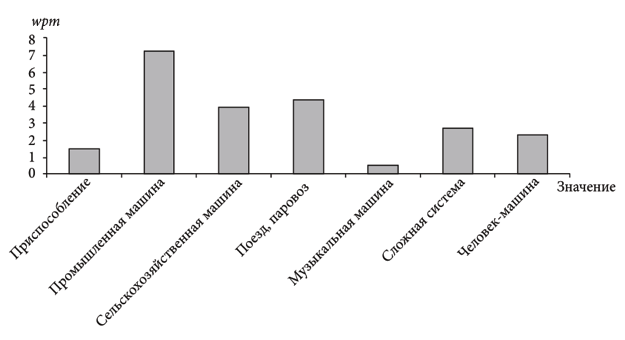
\includegraphics[width=0.8\textwidth]{img/book/mashina/1861-1890}
    \caption{Значения слова \textit{машина} для 1861-1890 согласно~\cite{TwoCenturies}}
    \label{fig:TwoCenturiesMashina1}
\end{figure}

\begin{figure}[H]
    \centering % Centers the images
    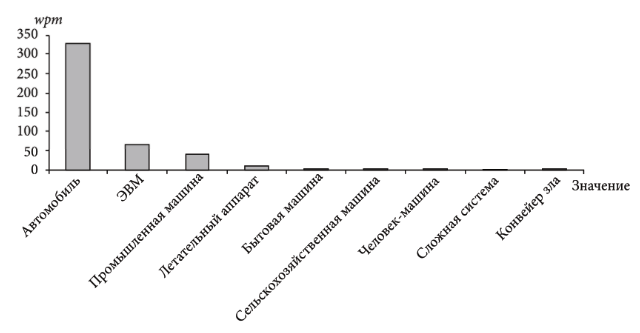
\includegraphics[width=0.8\textwidth]{img/book/mashina/1960-1970}
    \caption{Значения слова \textit{машина} для 1960-1970 согласно~\cite{TwoCenturies}}
    \label{fig:TwoCenturiesMashina2}
\end{figure}

Тем не менее, в книге обсуждается использование слова в значении ’Поезд, паровоз.’
в досоветский период, а также в значении ’Устройство для работы с информацией, компьютер’,
которые были не были выделены алгоритмом.

Таким образом, алгоритм в целом отражает значения, в которых использовалось
слово \textit{машина}, согласуясь с данными из толкового словаря и историческим исследованием.
Алгоритм выделяет изменение в частотности двух основных значения, но не вывел информацию по менее важным.

\section*{Молодец}

В результате анализа семем лексемы \textit{молодец} в толковых словарях были выделены пять групп значений,
которые можно условно сформулировать следующим образом:

\begin{enumerate}
    \item Молодой, крепкий, статный мужчина. \textit{Плечистый молодец.}
    (\textit{«Молодой человек, достигший расцвета лет, крепкий и статный.»} в БТС,
    \textit{«Молодой человек, сильный, крепкого сложения.»} в ТСО,  % TODO: Это не отдельное значение? (в примерах Разбойные молодцы. Ловкачи-молодцы.)
    \textit{«обычно мн. Человек, обычно сильный, смелый, бесшабашный.»} в ТСО
    \textit{«Молодцом называют молодого, здорового, привлекательного парня.»} в ТСД)

    \item Удалец, храбрец, герой (в народной словесности). \textit{Сказка про доброго молодца.}
    (\textit{«Сильный и смелый герой; удалец, храбрец.»} в БТС,
    \textit{«В народной словесности: удалец, храбрец.»} в ТСО)

    \item Похвала, одобрение чьих-либо действий. \textit{Какой же ты молодец.}
    (\textit{«О том, чьи действия вызвали одобрение, удовлетворение у кого-л.»} в БТС,
    \textit{«Выражение похвалы тому, кто делает что-н. хорошо, ловко, умело.»} в ТСО,
    \textit{«Молодцом вы называете того, чьи действия вы одобряете, хвалите.»} в ТСД,
    \textit{«Похвала»} в «Двух веках в двадцати словах»)

    \item Слуга, помощник, служащий. \textit{Молодцы в кладовой.}
(\textit{«Служащий»} в «Двух веках в двадцати словах»)

    \item Бандит или приспешник вражеских групп. \textit{Молодец из бандитской шайки.}
(\textit{«Пренебр. =Молодчик (3 зн.: Пособник, приспешник или участник каких-л. реакционных,
вражеских или преступных групп, организаций.).»} в БТС)
\end{enumerate}

%Кроме того, в словарях отмечено употребление слова \textit{молодец} по отношению к женщине в значении похвалы:
%\textit{«Употребление по отношению к женщине»} в «Двух веках в двадцати словах».

\begin{figure}[H]
	\centering
	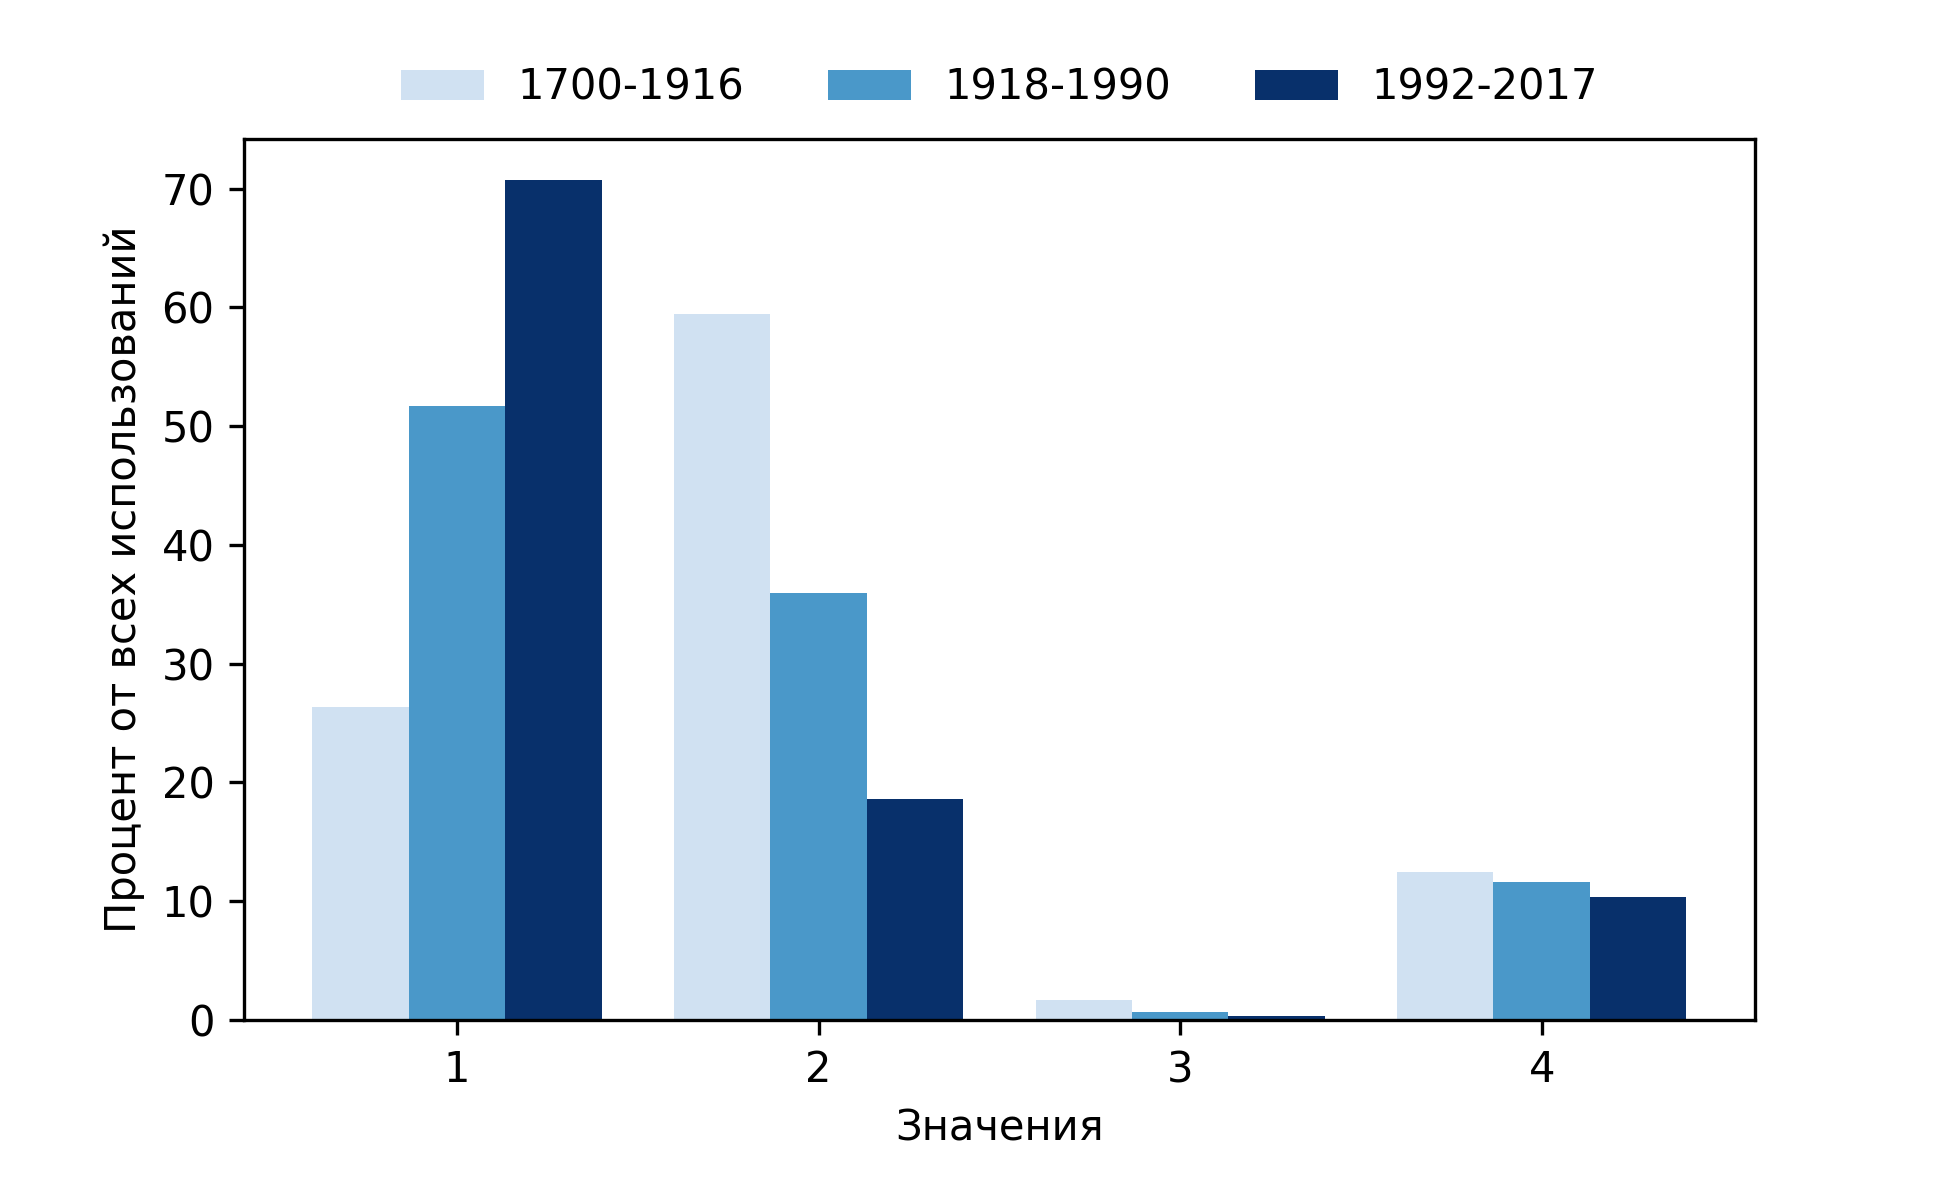
\includegraphics[width=0.8\textwidth]{img/visualizations/molodets_minimal}
	\caption{Изменение значений слова \textit{молодец}}
	\label{fig:Молодец}
\end{figure}

Значения для визуализации слова \textit{молодец} (Параметры: eps=0.19, min\_samples=5).

\begin{enumerate}
    \item Употребляется как похвала, одобрение.
    \item Молодой человек, юноша.
    \item Употребляется как бранное слово.
    \item О молодом человеке, отличающемся храбростью, удалью и т. п.
\end{enumerate}

\subsection*{Анализ значений слова \textit{молодец}}

Первые четыре определения в визуализации имеют следующие соответствия с обобщенными значениями из словарей:

\begin{itemize}
    \item ’Употребляется как похвала, одобрение.’
Это определение соответствует третьему обобщенному значению:
’Похвала, одобрение чьих-либо действий.’ Общие семы: \textit{’похвала’}, \textit{’одобрение’}.
Данный пример является корректным.

    \item ’Молодой человек, юноша.’
    Это определение соответствует первому обобщенному значению:
    ’Молодой, крепкий, статный мужчина.’
    Общие семы: \textit{’молодой’}, \textit{’человек’}.
    Хотя в определении визуализации отсутствуют семы \textit{’крепкий’} и \textit{’статный’}, это определение можно считать корректным, но недостаточно конкретизированным.

    \item ’Употребляется как бранное слово.’
    Это определение можно считать близким к пятому обобщенному значению:
    ’Бандит или приспешник вражеских групп.’
    Определения объединяет наличие негативной коннотации.

    \item ’О молодом человеке, отличающемся храбростью, удалью и т. п.’

    Это определение соответствует второму обобщенному значению:
    ’Удалец, храбрец, герой (в народной словесности).’
    Общие семы: \textit{’молодой человек’}, \textit{’храбрость’}, \textit{’удаль’}.
    Это определение можно считать корректным.

\end{itemize}

Обобщённые значения, не найденные в визуализации:

\begin{itemize}
    \item Слуга, помощник, служащий.

    Это значение отсутствует в визуализации.
    Возможно, это значение не достаточно распространено или редко упоминается в используемых данных.
\end{itemize}

\subsection*{Статистика по лексеме \textit{молодец}}
\begin{itemize}
    \item Корректные определения: 2
    \item Недостаточное конкретизирование: 1
    \item Близкое значение: 1
\end{itemize}

Таким образом, модель в целом корректно определяет основные значения слова \textit{молодец},
но не охватывает все возможные значения, представленные в словарях.

Перейдем к частотности значений.

Основным моментом, выделяемым книгой «Два века в двадцати словах», является
выход значения ’Похвала, одобрение чьих-либо действий.’ на лидирующие позиции
вместо изначального значения ’Молодой, крепкий, статный мужчина.’, что можно увидеть
графике~\ref{fig:TwoCenturiesMolodets}.
В визуализации, сделанной алгоритмом, это также отображено.
Значение ’Употребляется как похвала, одобрение.’ растёт с 30\% в досоветский период
растёт до 70\% в постсоветский за счёт уменьшения использования ’Молодой человек, юноша.’.
Также утверждается уменьшение использлвания значения ’Слуга, помощник, служащий.’,
который не был выделен алгоритмом.

\begin{figure}[H]
    \centering % Centers the images
    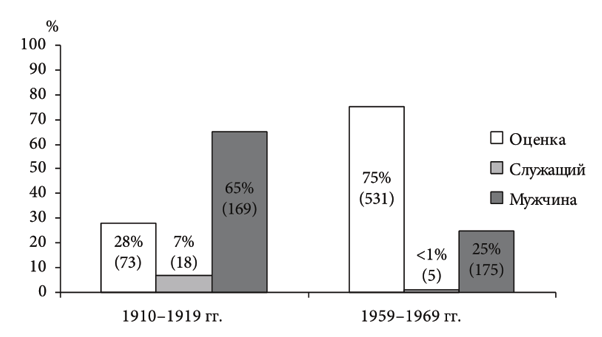
\includegraphics[width=0.7\textwidth]{img/book/molodets/1910-1969}
    \caption{Значения слова \textit{молодец} для 1910-1969 согласно~\cite{TwoCenturies}}
    \label{fig:TwoCenturiesMolodets}
\end{figure}

Таким образом, алгоритм в целом отражает значения, в которых использовалось
слово \textit{молодец}, согласуясь с данными из толкового словаря и историческим исследованием.
Алгоритм выделяет основных значения, но не вывел ’Слуга, помощник, служащий.’.

\section*{Передовой}

\begin{enumerate}
    \item Идущий, движущийся впереди остальных; ведущий. \textit{Передовая машина в автоколонне.}
(\textit{«Идущий, движущийся впереди остальных; ведущий.»} в БТС,
\textit{«Движущийся или находящийся впереди.»} в ТСО,
\textit{«Идущий впереди»} в «Двух веках в двадцати словах»)

    \item Находящийся, действующий впереди, в авангарде (о военных силах). \textit{Передовой отряд.}
(\textit{«Находящийся, действующий впереди, в авангарде (о военных силах).»} в БТС,
\textit{«В военном деле передовыми называют отряды, позиции и т. д., находящиеся ближе всего к месту боевых действий.»} в ТСД,
\textit{«Расположенный в авангарде» (о военных действиях)} в «Двух веках в двадцати словах»)

    \item Превосходящий других по уровню своего технического развития. \textit{Передовые достижения в освоении моря.}
(\textit{«Превосходящий других по уровню своего развития; прогрессивный.»} в БТС,
\textit{«Не останавливающийся в развитии, прогрессивный.»} в ТСО,
\textit{«Передовыми называют очень современные, сложные и интересные методы, технологии и т. д.»} в ТСД)

    \item Содержащий, излагающий прогресивные идеи, часто свободолюбивые, либеральные или демократические мысли. \textit{Передовые взгляды.}
(\textit{«Содержащий, излагающий свободолюбивые, либеральные мысли; демократический.»} в БТС,
\textit{«Прогрессивный»} в «Двух веках в двадцати словах»)

    \item Руководящая статья в газете, журнале, печатаемая на первом месте. \textit{Прочитайте передовую.}
(\textit{«Руководящая редакционная статья в газете, журнале, печатаемая на первом месте.»} в ТСО,
\textit{«Статья»} в «Двух веках в двадцати словах»)

    \item Превосходивший других по своим успехам в работе или опережавший других по производственным показателям. \textit{Колхоз, отстававший в прошлые годы по всем показателям, теперь выходит в передовые.}
(\textit{«В СССР: превосходивший других по своим успехам в работе или опережавший других по производственным показателям.»} в БТС,
\textit{«Передовым называли (во времена СССР) человека, коллектив и т. д., который достиг наибольших успехов в работе.»} в ТСД)

    \item Идеи, книги, способствующие какому-то развитию общества, науки, литературы. \textit{Фильм, передовой для своего времени, сейчас безнадёжно устарел.}
(\textit{«Передовыми называют новые современные идеи, книги, способствующие какому-то развитию общества, науки, литературы и т. п.»} в ТСД)

    \item Человек, отправленный для передачи информации или выполнения определенной миссии; посланник, гонец. \textit{Послал передовым.}
(\textit{«Посланник, гонец»} в «Двух веках в двадцати словах»)
\end{enumerate}

\begin{figure}[H]
	\centering
	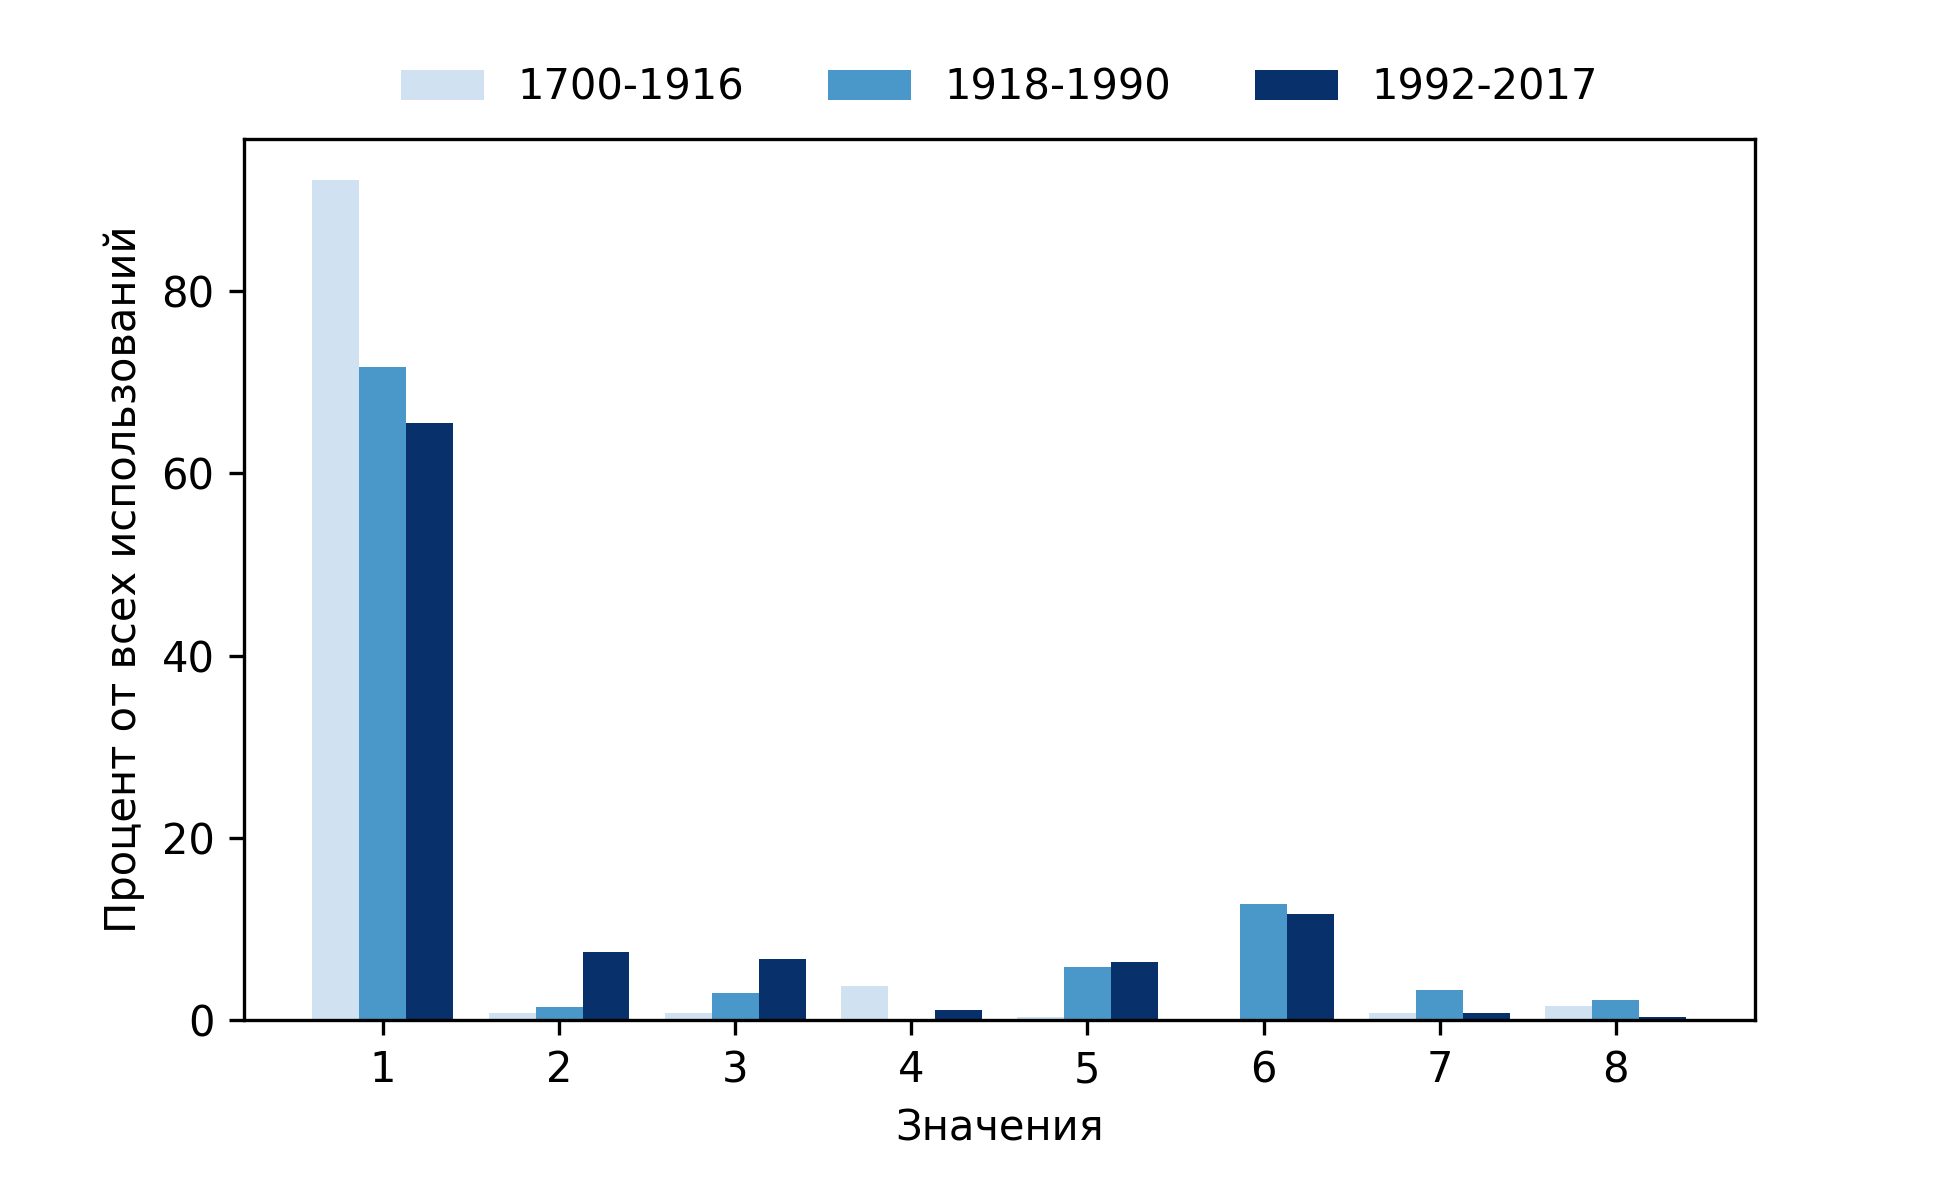
\includegraphics[width=0.8\textwidth]{img/visualizations/peredovoj_minimal}
	\caption{Изменение значений слова \textit{передовой}}
	\label{fig:Передовой}
\end{figure}

Значения для визуализации слова \textit{передовой} (Параметры: eps=0.18, min\_samples=12).

\begin{enumerate}
    \item Находящийся в авангарде, в первых рядах чего-либо.
    \item Основанный на новейших достижениях науки, техники и т. п.
    \item Содержащий в себе новое, прогрессивное.
    \item Являющийся передовицей.
    \item Передний край обороны, боевых действий.
    \item Передний край, линия фронта.
    \item Главная, основная часть газеты, журнала.
    \item Находящийся на более высокой ступени общественного развития по сравнению с другими.
\end{enumerate}

\subsection*{Анализ значений слова \textit{передовой}}

Первое и четвертое определения корректно сформулированы.
Второе и пятое определения не соответствуют обобщенным значениям.

\begin{itemize}
    \item ’Находящийся в авангарде, в первых рядах чего-либо.’ имеет общий смысловой элемент с
’Идущий, движущийся впереди остальных; ведущий.’,
а именно семы \textit{’находящийся’}, \textit{’в авангарде/в первых рядах’}.

    \item ’Основанный на новейших достижениях науки, техники и т. п.’ полностью соответствует
’Превосходящий других по уровню своего технического развития.’,
так как включает те же семы \textit{’новейшие достижения’}, \textit{’наука, техника’}.

    \item ’Содержащий в себе новое, прогрессивное.’ имеет общий смысловой элемент с
’Содержащий, излагающий прогрессивные идеи, часто свободолюбивые, либеральные или демократические мысли.’,
а именно семы \textit{’содержащий’}, \textit{’новое/прогрессивное’}, однако представляет собой более широкое
определение, так как не ограничивается только идеями.

    \item ’Являющийся передовицей.’ и ’Главная, основная часть газеты, журнала.’ полностью соответствуют
’Руководящая статья в газете, журнале, печатаемая на первом месте.’, так как семы \textit{’главная/основная’}, \textit{’часть газеты, журнала/статья’} полностью отражают смысл ’руководящая статья’.
\end{itemize}

\begin{itemize}
    \item ’Передний край обороны, боевых действий.’ и ’Передний край, линия фронта.’
вместе имеют частичное соответствие с ’Находящийся, действующий впереди, в авангарде (о военных силах).’,
так как семы \textit{’передний край/в авангарде’}, \textit{’боевых действий/военных сил’} частично отражают смысл «впереди, в авангарде».
Однако данное определение ближе подходит к значению субстантивированного прилагательного \textit{передовая} –
’Участок оборонительной линии, соприкасающейся с неприятельским фронтом; передовая линия.’.
Например, для контекста \textit{Такое случилось еще раз, потому что отказать во встрече уходящему на передовую,
когда к Москве подступают немцы, было невозможно.} было сгенерировано ’Передний край обороны, боевых действий.’.
Исследуемые определения будут считаться нами как корректные.
\end{itemize}

Обобщённые значения, не найденные в визуализации:
\begin{itemize}
    \item ’Превосходивший других по своим успехам в работе или опережавший других по производственным показателям.’
отсутствует среди предложенных моделью значений.
Можно предположить, что информации из контекста использований недостаточно для отделения этого значения от
’Превосходящий других по уровню своего развития; прогрессивный.’. % TODO: проверить

    \item ’Человек, отправленный для передачи информации или выполнения определенной миссии; посланник, гонец.’ также отсутствует в визуализации.
%Однако, модель способна на выделение данного значения.
\end{itemize}

Таким образом, для лексемы \textit{передовой} представлено 7 корректных определений.
Среди ошибок присутствуют:
\begin{itemize}
    \item Недостаточное конкретизирование: 1
\end{itemize}

Перейдем к частотности значений.

В книге лишь значение ’Основанный на новейших достижениях науки, техники и т. п.’
указывается как появивишееся после 1917 года, что подтверждается
в визуализации алгоритма, где оно представлено только в советский и постсоветский период.
Кроме того, указано, что военное значение ’Находящийся в авангарде, в первых рядах чего-либо.’
уступает переносным значениям, акцентирующимся на прогрессивности, чего
не наблюдается в визуализации, сделанной алгоритмом.

Снизу расположены графики из книги «Два века в двадцати словах»
для 1830-1859 гг.~\ref{fig:TwoCenturiesPeredovoj1} и 1930-1939 гг.~\ref{fig:TwoCenturiesPeredovoj2}.

\noindent % Prevents indentation for this line to align the images at the left margin
\begin{figure}[H]
    \centering % Centers the images
    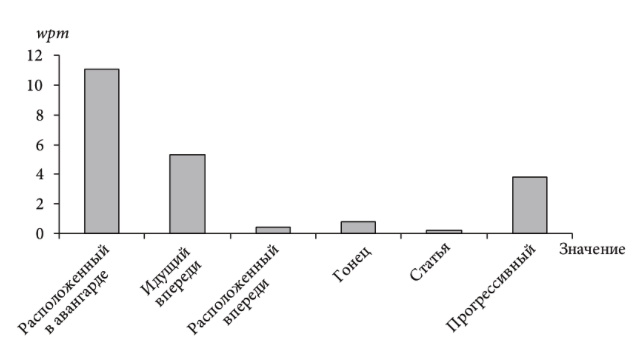
\includegraphics[width=0.8\textwidth]{img/book/peredovoj/1830-1859}
    \caption{Значения слова \textit{передовой} для 1830-1859 согласно~\cite{TwoCenturies}}
    \label{fig:TwoCenturiesPeredovoj1}
\end{figure}

\begin{figure}[H]
    \centering % Centers the images
    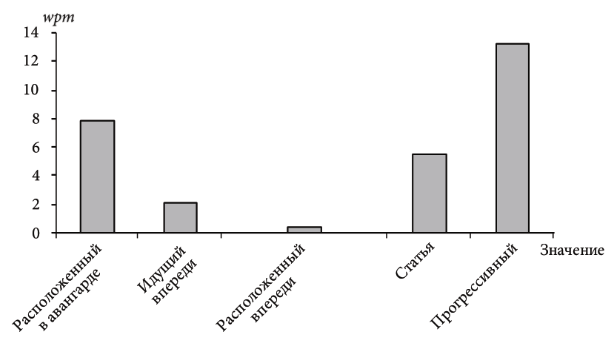
\includegraphics[width=0.8\textwidth]{img/book/peredovoj/1930-1939}
    \caption{Значения слова \textit{передовой} для 1930-1939 согласно~\cite{TwoCenturies}}
    \label{fig:TwoCenturiesPeredovoj2}
\end{figure}

Таким образом, нельзя сказать, что алгоритм отражает значения, в которых использовалось
слово \textit{передовой}, так как они не полностью согласуются
с данными из толкового словаря и историческим исследованием.

\section*{Пионер}

\begin{enumerate}
    \item Человек, впервые проникший в неисследованную страну, область и поселившийся в ней. \textit{Пионеры Америки, Сибири, Австралии.}
(\textit{«Человек, впервые проникший в неисследованную страну, область и поселившийся в ней.»} в БТС,
\textit{«Человек, к-рый одним из первых пришел и поселился в новой неисследованной стране, местности.»} в ТСО,
\textit{«Первый поселенец на какой-либо территории»} в «Двух веках в двадцати словах»)

    \item Тот, кто положил начало чему-либо в какой-либо сфере деятельности, в науке, культуре; новатор, зачинатель. \textit{Пионер естествознания.}
(\textit{«Тот, кто прокладывает новые пути в какой-л. сфере деятельности, в науке, культуре; новатор, зачинатель.»} в БТС,
\textit{«Человек, к-рый положил начало чему-н. новому в области науки, культуры »} в ТСО,
\textit{«Первооткрыватель»} в «Двух веках в двадцати словах»)

    \item Член добровольной самодеятельной детской организации. \textit{Вступить, принять в пионеры.}
(\textit{«В СССР: член добровольной самодеятельной детской организации, объединявшей детей и подростков от 10 до 15 лет.»} в БТС,
\textit{«Член детской организации в СССР и ряда детских организаций в нек-рых других странах.»} в ТСО,
\textit{«Член детской организации»} в «Двух веках в двадцати словах»)

    \item Военная профессия, связанная с разминированием, строительством мостов и укреплений. \textit{К построению мостов и укреплений посланы инженеры и пионеры.}
(\textit{«Сапер.»} в «Двух веках в двадцати словах»)
\end{enumerate}

\begin{figure}[H]
	\centering
	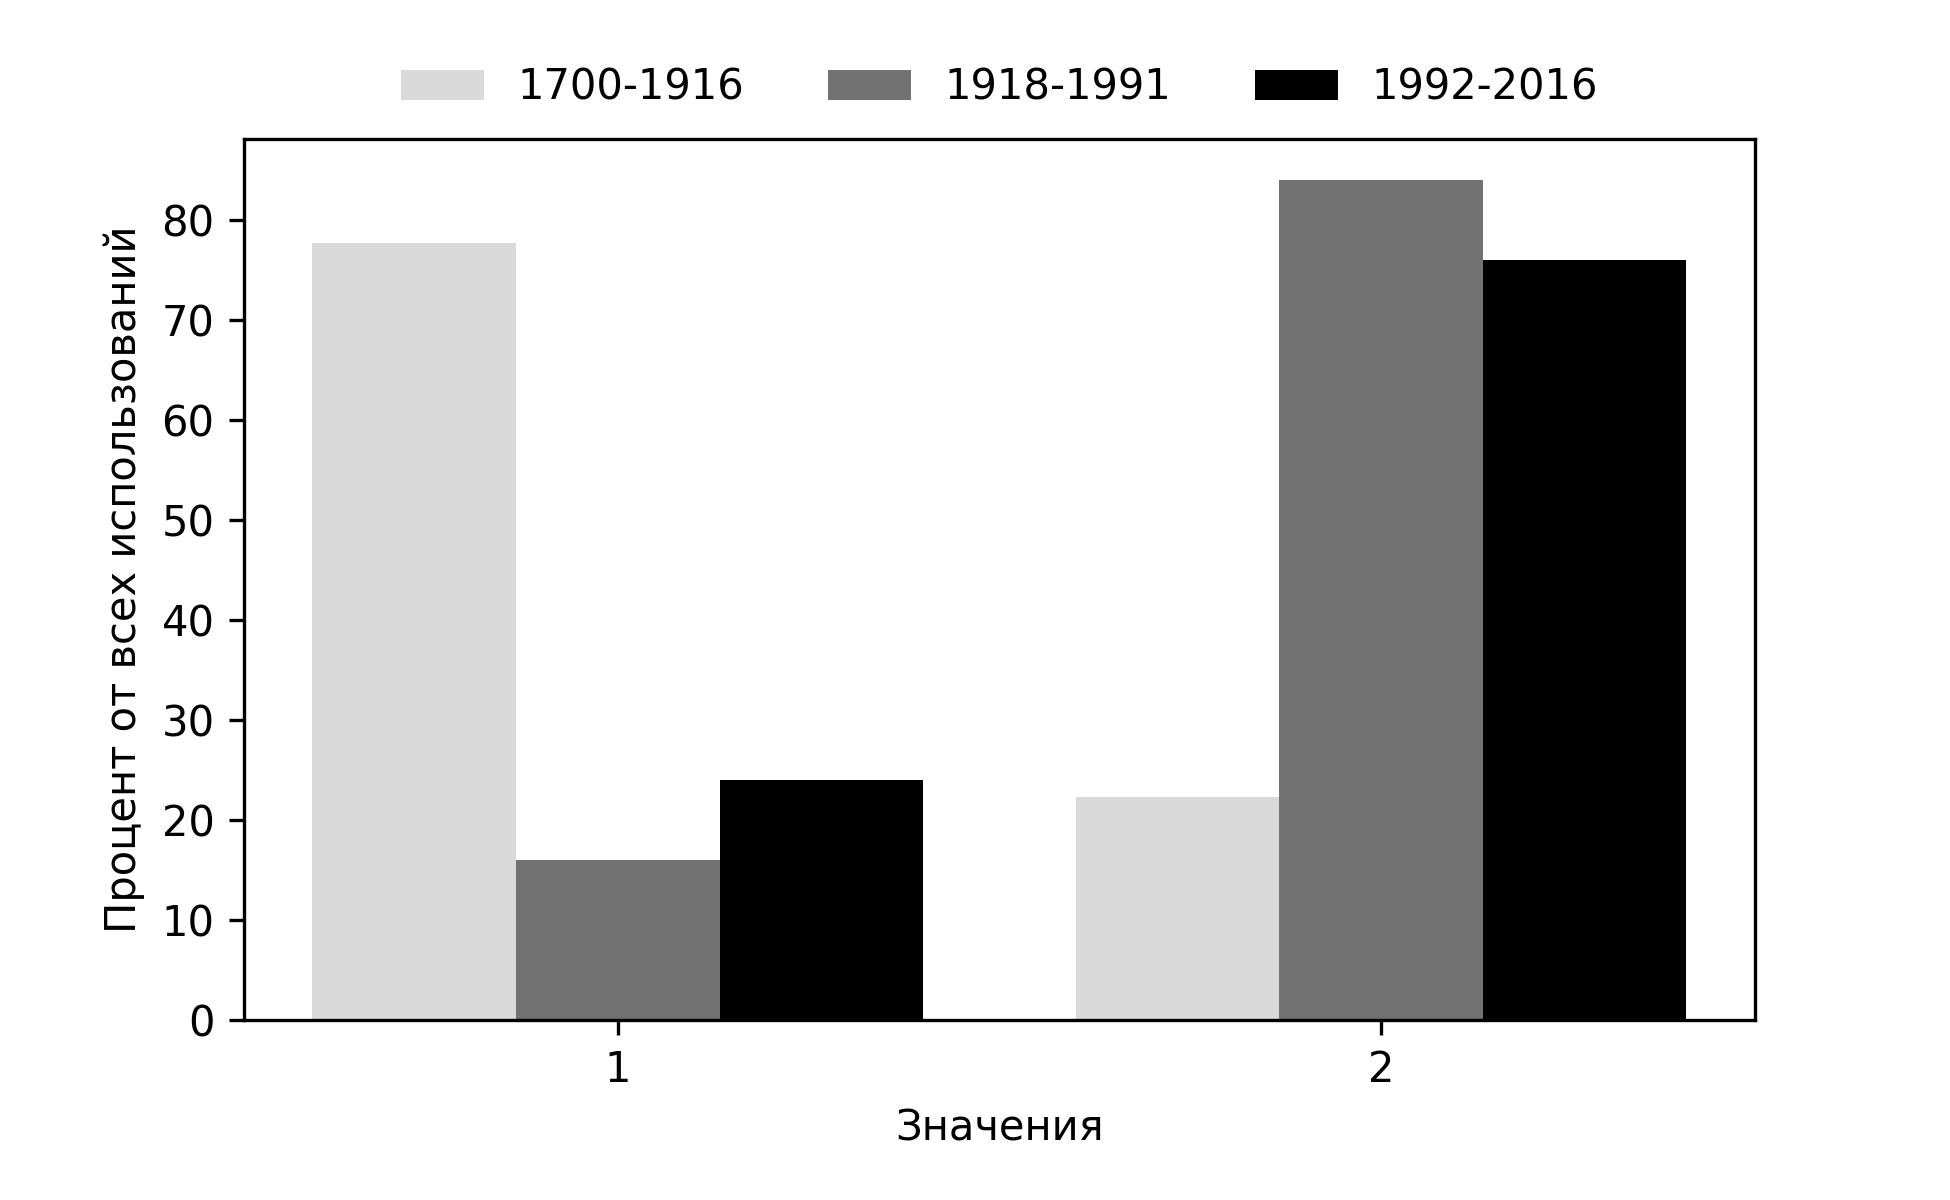
\includegraphics[width=0.8\textwidth]{img/visualizations/pioner_minimal}
	\caption{Изменение значений слова \textit{пионер}}
	\label{fig:Пионер}
\end{figure}

Значения для визуализации слова \textit{пионер} (Параметры: eps=0.18, min\_samples=15).

\begin{enumerate}
    \item Тот, кто первым начал что-либо делать, кто является основоположником чего-либо.
    \item Юный член пионерской организации.
\end{enumerate}

\subsection*{Анализ значений слова \textit{пионер}}

Оба определения корректно сформулированы.

\begin{itemize}
    \item ’Тот, кто первым начал что-либо делать, кто является основоположником чего-либо.’ имеет общий смысловой элемент с
’Тот, кто положил начало чему-либо в какой-либо сфере деятельности, в науке, культуре; новатор, зачинатель.’,
а именно семы \textit{’начало’}, \textit{’деятельность’}, \textit{’новаторство’}.

    \item ’Юный член пионерской организации.’ полностью соответствует
’Член добровольной самодеятельной детской организации.’, так как включает те же семы \textit{’член’}, \textit{’детская организация’}.
\end{itemize}

Обобщённые значения, не найденные в визуализации:
\begin{itemize}
    \item ’Человек, впервые проникший в неисследованную страну, область и поселившийся в ней.’
отсутствует среди предложенных моделью значений.
В книге «Два века в двадцати словах» указывается, что это в русском имело единичные использования.
Можно предположить, что оно не вошло в исследуемую выборку.
%Однако, модель способна на выделение данного значения.  % TODO: проверить

    \item ’Военная профессия, связанная с разминированием, строительством мостов и укреплений.’ также отсутствует в визуализации.
В книге «Два века в двадцати словах» указывается, что это значение редкое.
Можно предположить, что оно не вошло в исследуемую выборку.
%Однако, модель способна на выделение данного значения.  % TODO: проверить
\end{itemize}

Таким образом, для лексемы \textit{пионер} представлено 2 корректных определения.

Перейдем к частотности значений.

Значения, связанные с первооткрывательством, а также с сапёром, появились до 1917 года.
Новым значением является ’Член добровольной самодеятельной детской организации.’,
появившееся в советское время.
В визуализации алгоритма указано около 20\% использований слова в таком значении
в досоветский период, что объясняется двусмысленностью части примеров,
например, \textit{«Пионеры слушают это и восхищаются.»}, где необходим дополнительный контекст
для установления значения.

\begin{figure}[H]
    \centering % Centers the images
    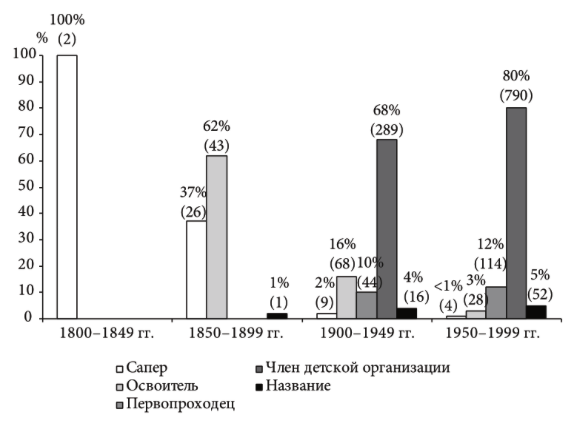
\includegraphics[width=0.8\textwidth]{img/book/pioner/all}
    \caption{Значения слова \textit{пионер} согласно~\cite{TwoCenturies}}
\end{figure}

Таким образом, алгоритм лишь частично отражает значения, в которых использовалось
слово \textit{пионер}, так как из 4 значений выделено только 2, из которых
около 20\% размечено неверно.

\section*{Пожалуй}

\begin{enumerate}
    \item Выражение допущения или вероятности. \textit{Было уже, пожалуй, за полночь.}
(\textit{«Вводное слово, выражающее допущение возможного, склонность согласиться.»} в ТСО,
\textit{«Словом пожалуй обозначают вероятность чего-либо.»} в ТСД,
\textit{«Возможно.»} в «Двух веках в двадцати словах»)

    \item Выражение намерения совершить действие. \textit{Я, пожалуй, пойду.}
(\textit{«Слово пожалуй употребляется в том случае, если кто-либо сообщает о своём намерении
совершить какое-либо действие, которое кажется этому человеку наиболее приемлемым в какой-либо ситуации.»} в ТСД,
\textit{«Склоняюсь к тому, что...»} в «Двух веках в двадцати словах»)

    \item Выражение нерешительного, неопределённого согласия. \textit{Чайку не хотите? — Пожалуй.}
(\textit{«Частица, выражающая не уверенное согласие.»} в ТСО,
\textit{«Словом пожалуй обозначают нерешительное, неопределённое согласие что-либо сделать.»} в ТСД,
\textit{«Ладно, согласен.»} в «Двух веках в двадцати словах»)

    \item Вежливое обращение или просьба. \textit{Пожалуй-ка, мой друг, потрудись и поспеши челобитную написать и будь уверен, что я буду тебе благодарен.}
(\textit{«Повелительный наклон, при вежливом обращении.»} в БТС,
\textit{«Будь добр.»} в «Двух веках в двадцати словах»)
\end{enumerate}

\begin{figure}[H]
	\centering
	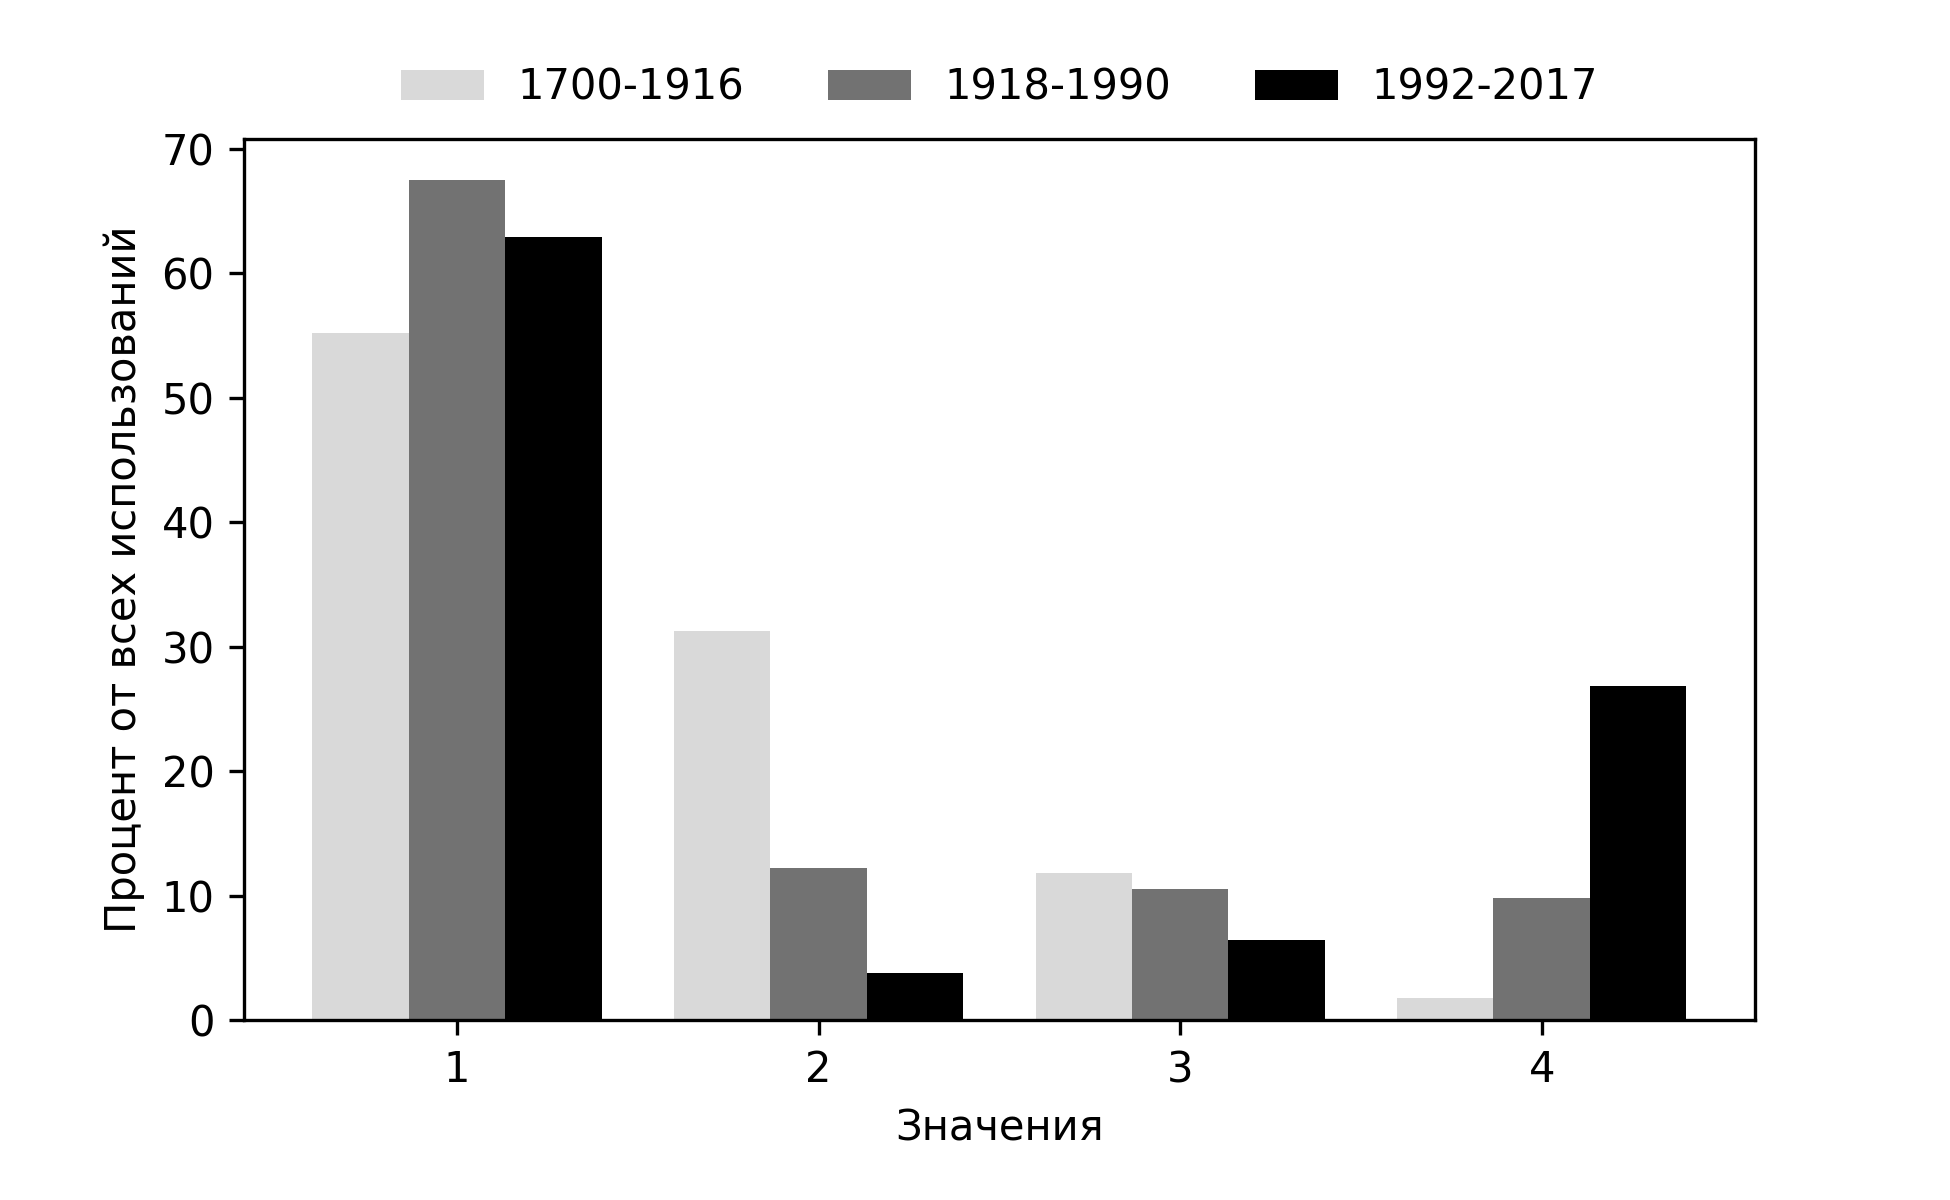
\includegraphics[width=0.8\textwidth]{img/visualizations/pozhaluj_minimal}
	\caption{Изменение значений слова \textit{пожалуй}}
	\label{fig:Пожалуй}
\end{figure}

Значения для визуализации слова \textit{пожалуй} (Параметры: eps=0.15, min\_samples=10).

\begin{enumerate}
    \item Употребляется для выражения сомнения, неуверенности в чем-либо.
    \item Употребляется для выражения просьбы, приглашения к чему-либо.
    \item Вполне возможно, вероятно.
    \item Употребляется для присоединения предложений или отдельных членов предложений,
усиливающих или уточняющих высказанную мысль.
\end{enumerate}

\subsection*{Анализ значений слова \textit{пожалуй}}

Первое, второе и третье определения корректно сформулированы.
Четвертое определения не соответствуют обобщенным значениям.

\begin{itemize}
    \item ’Употребляется для выражения сомнения, неуверенности в чем-либо.’
не имеет похожих обобщенных определений, а примеры, которые имеют данное определение,
например, \textit{«От отца я, пожалуй, кроме книг ничего в подарок и не получал.»}
было бы корректно отнести к ’Вполне возможно, вероятно.’
%имеет общий смысловой элемент с ’Выражение нерешительного, неопределённого согласия.’,
%а именно семы «сомнение» и «неуверенность», но не имеет семы «согласия».

    \item ’Употребляется для выражения просьбы, приглашения к чему-либо.’ соответствует
’Вежливое обращение или просьба’ с общими семами \textit{’просьбы’}.

    \item ’Вполне возможно, вероятно.’ соответствует
’Выражение допущения или вероятности.’, так как включает те же семы \textit{’возможности’}, \textit{’вероятности’}.
\end{itemize}

\begin{itemize}
    \item ’Употребляется для присоединения предложений или отдельных членов предложений,
усиливающих или уточняющих высказанную мысль.’ является некорректным значением,
так как описывает такое функциональное использование в синтаксисе, что отсутствует в словарях.
\end{itemize}

Обобщённые значения, не найденные в визуализации:
\begin{itemize}
    \item ’Выражение намерения совершить действие’ также отсутствует в визуализации.
%Однако, модель способна на выделение данного значения. % TODO: прогнать на примере модель
\end{itemize}

Таким образом, для лексемы \textit{пожалуй} представлено 2 корректных определения.
Среди ошибок присутствуют:
\begin{itemize}
    \item Некорректность определений: 2
\end{itemize}

Перейдем к частотности значений.

В книге сообщается, что изначальные значения ’Вежливое обращение или просьба’
и ’Выражение нерешительного, неопределённого согласия.’ были вытсенены в течение XIX века
преобладающим на сегодняшний момент значением ’Вполне возможно, вероятно.’
В визуализации данная информация подтверждается для значения
’Употребляется для выражения просьбы, приглашения к чему-либо.’,
имевшее в постсовесткий период более 30\% использований и около 5\% в постсовесткий.
Тем не менее, затруднительно установить корректность статистики далее из-за
некорректных определений.

Информация из книги «Два века в двадцати словах» находится на графиках~\ref{fig:TwoCentrutiesPozhaluj1} и~\ref{fig:TwoCentrutiesPozhaluj2}.

\noindent % Prevents indentation for this line to align the images at the left margin
\begin{figure}[H]
    \centering % Centers the images
    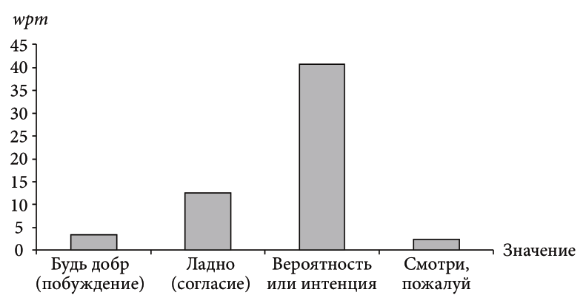
\includegraphics[width=0.8\textwidth]{img/book/pozhaluj/1831-1860}
    \caption{Значения слова \textit{пожалуй} для 1831-1860 согласно~\cite{TwoCenturies}}
    \label{fig:TwoCentrutiesPozhaluj1}
\end{figure}

\begin{figure}[H]
    \centering % Centers the images
    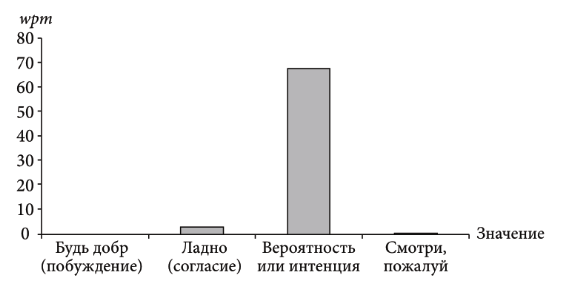
\includegraphics[width=0.8\textwidth]{img/book/pozhaluj/1900-1910}
    \caption{Значения слова \textit{пожалуй} для 1900-1910 согласно~\cite{TwoCenturies}}
    \label{fig:TwoCentrutiesPozhaluj2}
\end{figure}

Таким образом, алгоритм лишь частично отражает значения, в которых использовалось
слово \textit{пожалуй}, так как из 4 значений корректны только 2.

\section*{Привет}

\begin{enumerate}
    \item Вежливо-фамильярная форма приветствия при встрече или расставании. \textit{Привет, Алёша, как я рад тебя видеть!}
(\textit{«Дружеское или фамильярное приветствие, обращённое к кому-л. при встрече или расставании.»} в БТС,
\textit{«Приветствие при встрече или расставании.»} в ТСРЯ,
\textit{«Если кто-либо говорит Привет! при встрече с каким-либо человеком или группой людей,
значит, он просто употребляет вежливо-фамильярную форму приветствия.»} в ТСД,
\textit{«Здравствуйте».} в «Двух веках в двадцати словах»)

    \item Обращение к кому-либо с выражением дружеского расположения, дружеских чувств, доброжелательства. \textit{Сердечный, искренний привет.}
(\textit{«Обращённое к кому-л. выражение дружеского расположения, дружеских чувств, доброжелательства.»} в БТС,
\textit{«Обращенное к кому-н. выражение чувства личной приязни, доброго пожелания, солидарности.»} в ТСРЯ,
\textit{«Словесное или несловесное выражение внимания к собеседнику.»} в «Двух веках в двадцати словах»)

    \item Выражение удивления, несогласия, иронии. \textit{Я не понимаю. - Привет, ну, ты даёшь.}
(\textit{«Выражение удивления, несогласия, иронии.»} в БТС,
\textit{«Выражение недоумения, удивленного несогласия.»} в ТСРЯ,
\textit{«Если один человек говорит Привет! другому в ответ на какие-либо
не понравившиеся ему слова или действия, значит, он тем самым выражает удивление, несогласие, иронию.»} в ТСД)

    \item Формула заключения письма с выражением внимания к собеседнику. \textit{С приветом, друзья!}
(\textit{«С приветом, друзья! Ну я ухожу, п.! С дружеским, сердечным, большим и т.п. приветом;
с приветом (заключительная формула письма).»} в БТС,
\textit{«Иногда слова С (большим, пламенным и т. п.) приветом используются в качестве
формально-вежливой заключительной фразы в письме.»} в ТСД,
\textit{«Формула конца письма с выражением внимания к адресату письма.»} в «Двух веках в двадцати словах»)

%    \item Отсутствие ответа или реакции на обращение. \textit{Ни ответа ни привета. }
%(\textit{«Ни ответа ни привета. Об отсутствии ответа, отзыва на чьё-л. обращение, письмо.»} в БТС,
%\textit{«Ни ответа ни привета - нет никакого ответа от кого-н., никаких известий о ком-н.»} в ТСРЯ,
%\textit{«Говоря, что от кого-либо не слышно ни ответа, ни привета,
%вы подразумеваете под этим долгое отсутствие какого-либо отклика со стороны этого человека
%на ваше обращение, письмо.»} в ТСД)

%    \item Описание состояния человека, ведущего себя странно или глуповато.
%(\textit{«С приветом, в зн. прил. Разг. Со странностями, глуповатый или не совсем нормальный (о человеке).»} в БТС,
%\textit{«С приветом кто (прост.) - со странностями, не совсем нормален.»} в ТСРЯ,
%\textit{«Если вы говорите, что кто-либо (совсем) с приветом!, вы в грубоватой или ироничной форме
%выражаете своё мнение о том, что этот человек — со странностями, глуповат или не совсем нормален,
%или ведёт себя таким образом в данной ситуации.»} в ТСД)

    \item Формула выражения внимания к третьему лицу. \textit{Привет от меня всем знакомым в Вашем гарнизоне.}
(\textit{«Формула конца письма с выражением внимания к третьему лицу.»} в «Двух веках в двадцати словах»)

    \item Дружелюбное, ласковое обращение с кем-либо. \textit{С начала владения моего крестьянами положил себе правило, чтоб с ними обращаться простосердечно и откровенно, веселым видом, больше ласковостью и приветом.}
(\textit{Дружелюбное, ласковое обращение с кем-либо.} в «Двух веках в двадцати словах»)
\end{enumerate}

\begin{figure}[H]
	\centering
	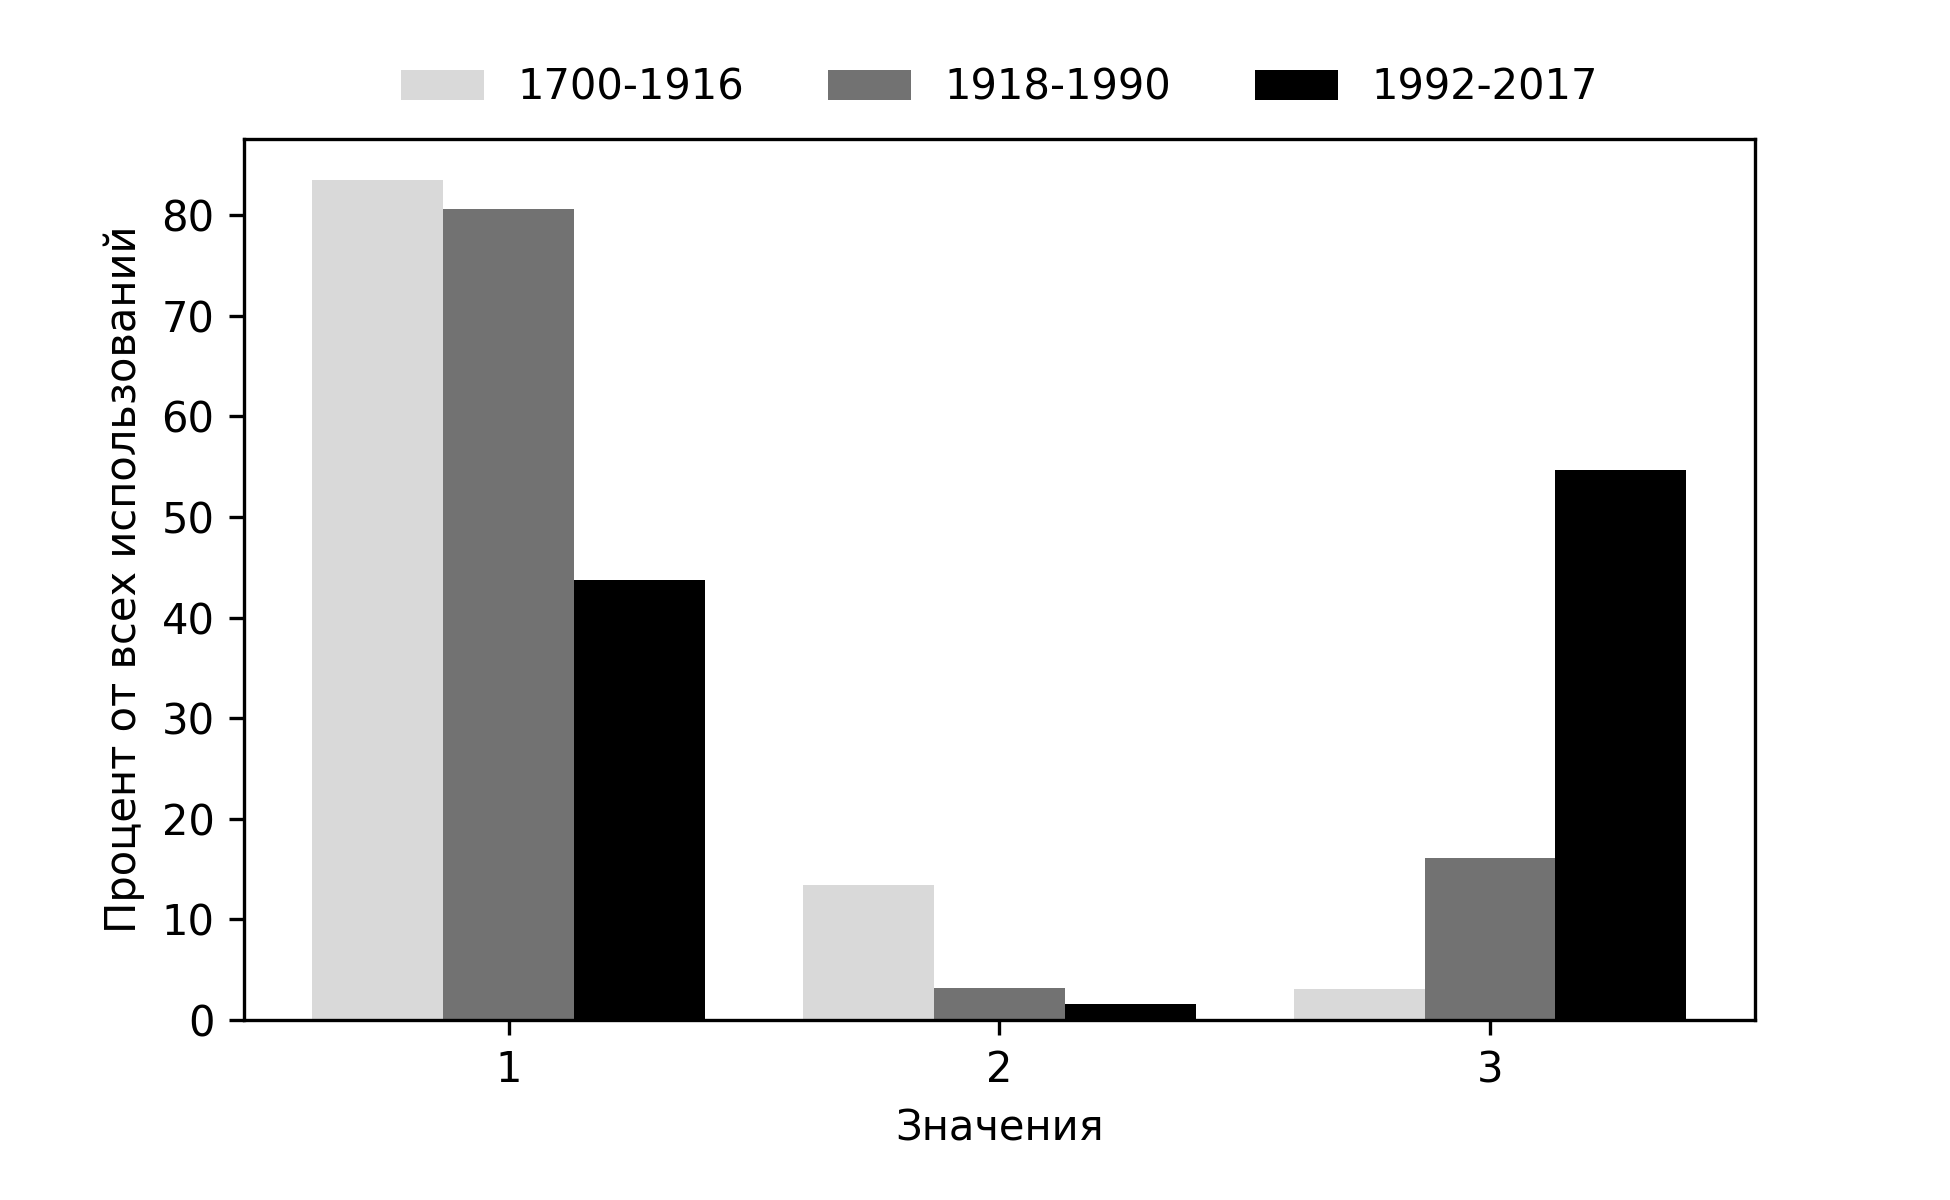
\includegraphics[width=0.8\textwidth]{img/visualizations/privet_minimal}
	\caption{Изменение значений слова \textit{привет}}
	\label{fig:Привет}
\end{figure}

Значения для визуализации слова \textit{привет} (Параметры: eps=0.1, min\_samples=20).

\begin{enumerate}
    \item Устное или письменное обращение к кому-либо с пожеланием доброго здоровья, счастья, успехов и т. п.
    \item Доброжелательное отношение к кому-, чему-либо.
    \item Добрый день, доброе утро.
\end{enumerate}

\subsection*{Анализ значений слова \textit{привет}}

Первое и третье определения корректно сформулированы.
Второе определение имеет обобщенное значение и соответствует конкретным значениям из словарей.

\begin{itemize}
    \item ’Устное или письменное обращение к кому-либо с пожеланием доброго здоровья, счастья, успехов и т. п.’
имеет общий смысловой элемент с ’Обращение к кому-либо с выражением дружеского расположения,
дружеских чувств, доброжелательства.’, а именно семы \textit{’обращение’} и \textit{’доброжелательность’}.

    \item ’Доброжелательное отношение к кому-, чему-либо.’ соответствует значению
’Дружелюбное, ласковое обращение с кем-либо.’,
так как включает те же семы \textit{’доброжелательность/дружелюбность’} и \textit{’отношение/обращение’}.

    \item ’Добрый день, доброе утро.’ соответствует значению
’Вежливо-фамильярная форма приветствия при встрече или расставании.’,
так как представляет из себя синонимичный ряд форм приветствия при встрече.
\end{itemize}

Обобщённые значения, не найденные в визуализации:
\begin{itemize}
    \item ’Выражение удивления, несогласия, иронии.’ отсутствует среди предложенных моделью значений.
%    Можно предположить, что информации из контекста использований недостаточно для отделения
%    этого значения от общего «доброжелательного обращения».
    Можно предположить, что это значение недостаточно часто встречается в исследуемой выборке,
либо модель неспособна на его выделение.

    \item ’Формула заключения письма с выражением внимания к собеседнику.’ и ’Формула выражения внимания к третьему лицу.’ также отсутствуют в визуализации.
%    Однако, модель способна на выделение данных значений при более детализированном контексте.

%    \item ’Отсутствие ответа или реакции на обращение.’ отсутствует среди предложенных моделью значений.
%    Это может быть связано с недостаточной частотностью данного значения в корпусе данных.
%
%    \item ’Описание состояния человека, ведущего себя странно или глуповато.’ также отсутствует в визуализации.
%    Причиной может быть ограниченность контекста или недостаточная выраженность данной семы в корпусе.
\end{itemize}

Таким образом, для лексемы \textit{привет} представлено 3 корректных определения:

Перейдем к частотности значений.

Судя по книге «Два века в двадцати словах» (график снизу), изначальные использования слова \textit{привет}
имели значения ’Обращение к кому-либо с выражением дружеского расположения,
дружеских чувств, доброжелательства.’ и ’Дружелюбное, ласковое обращение с кем-либо.’,
где первое значение было более распространено.
Ближе к завершению советского периода и после на первое место выходит использование
слова \textit{привет} как аналог \textit{здравствуйте}.
Все эти данные подкрепляются в нашей визуализации, где значение ’Добрый день, доброе утро.’
растёт с меньше 5\% в досоветский период до около 55\% в постсоветский, вытесняя
’Устное или письменное обращение к кому-либо с пожеланием доброго здоровья, счастья, успехов и т. п.’
с около 80\% до 45\% и ’Доброжелательное отношение к кому-, чему-либо.’ с 15\% до 2-3\%.
Более того, на графике~\ref{fig:TwoCenturiesPrivet} из книги заметно, что использование ’Доброжелательное отношение к кому-, чему-либо.’
снижается уже в начале советского периода, что так же отражено в нашей визуализации.

\begin{figure}[H]
    \centering % Centers the images
    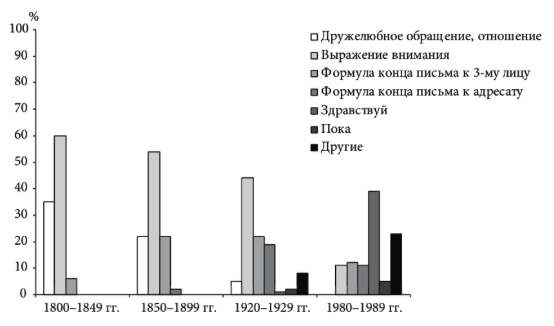
\includegraphics[width=0.8\textwidth]{img/book/privet/all}
    \caption{Значения слова \textit{привет} согласно~\cite{TwoCenturies}}
    \label{fig:TwoCenturiesPrivet}
\end{figure}

Таким образом, алгоритм отражает основные значения, в которых использовалось
слово \textit{привет}, согласуясь с данными из толкового словаря и историческим исследованием.

\section*{Пружина}

\begin{enumerate}
    \item Упругая узкая металлическая пластина или нить, согнутая преимущественно в форме спирали. \textit{Пружины матраца, дивана.}
(\textit{«Узкая упругая металлическая пластина или закрученная спиралью металлическая нить
(служащая обычно для приведения в действие механизмов, амортизации ударов и т.п.)»} в БТС,
\textit{«Упругая узкая металлическая пластина или нить, согнутая преимущ. спиралью.»} в ТСО,
\textit{«Он носил маску с железною пружиною, которая не мешала ему есть.»} в «Двух веках в двадцати словах»)

    \item Переносно, движущая сила в каком-то деле. \textit{Главная движущая пружина.}
(\textit{«Движущая сила в каком-н. деле.»} в ТСО, \textit{«Движущая сила чего-л.»} в БТС
\textit{«Природа есть первоначальная всему причина и самодвижущаяся пружина.»} в «Двух веках в двадцати словах»)

    \item Метафора сжатости, а именно, упругость как свойство объекта или субъекта. \textit{Пружины этой души были еще слабы и не расслаблены частым употреблением.}
(\textit{«Метафора сжатости (движения).»} в «Двух веках в двадцати словах»)
\end{enumerate}

\begin{figure}[H]
	\centering
	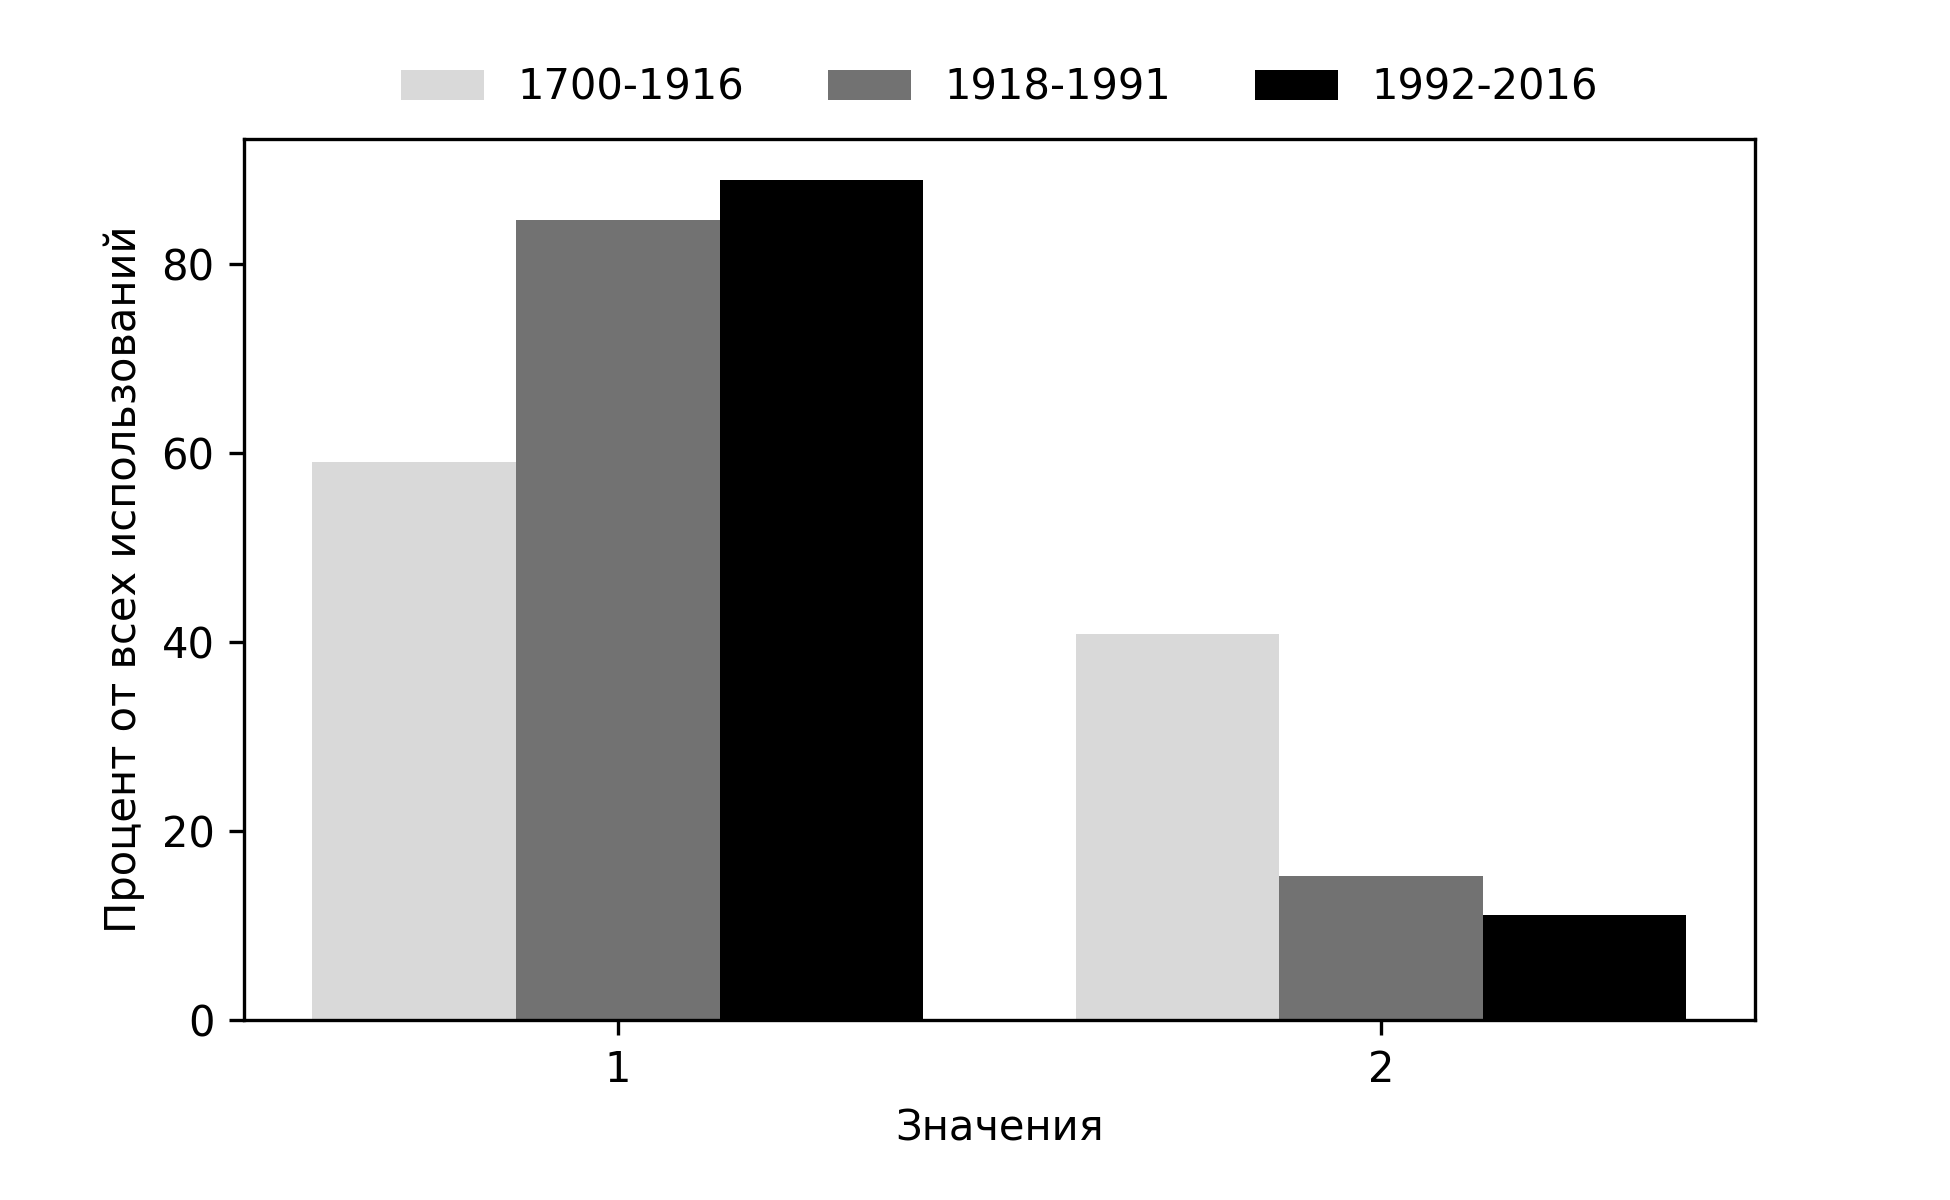
\includegraphics[width=0.8\textwidth]{img/visualizations/pruzhina_minimal}
	\caption{Изменение значений слова \textit{Пружина}}
	\label{fig:Пружина}
\end{figure}

Значения для визуализации слова \textit{пружина} (Параметры: eps=0.25, min\_samples=50).

\begin{enumerate}
    \item Механизм, приводимый в действие сжатием и разжатием упругого стержня.
    \item То, что является движущей силой, источником чего-либо.
\end{enumerate}

\subsection*{Анализ значений слова \textit{машина}}

Первое и второе определения корректно сформулированы.

\begin{itemize}
    \item ’Механизм, приводимый в действие сжатием и разжатием упругого стержня.’ имеет общий смысловой элемент с
’Упругая узкая металлическая пластина или нить, согнутая преимущественно в форме спирали.’, а именно семы \textit{’механизм’}, \textit{’упругость’}, \textit{’сжатие/разжатие’}, \textit{’стержень’}.

    \item ’То, что является движущей силой, источником чего-либо.’ полностью соответствует
’Переносно, движущая сила в каком-то деле.’, так как включает те же семы \textit{’движущая сила’}, \textit{’источник’}.
\end{itemize}

\begin{itemize}
    \item Метафорическое значение ’Метафора сжатости, а именно, упругость как свойство объекта или субъекта.’ не представлено в визуализации.
Это значение указано только в книге «Два века в двадцати словах» как самое редкое для всех периодов.
Вероятно, оно недостаточно распространено в исследуемом материале, поэтому не вошло в визуализацию.
\end{itemize}

Таким образом, для лексемы \textit{пружина} представлено 2 корректных определения.

Перейдем к частотности значений.

В книге «Два века в двадцати словах» (графики ниже) сообщается о постепенной замене
преобладающего метафорического значения слова (’Переносно, движущая сила в каком-то деле.’)
на прямое (’Упругая узкая металлическая пластина или нить, согнутая преимущественно в форме спирали.’)
в конце XIX века и о нынешнем преобладании прямого значения.
Такие же данные представлены в нашей визуализации, где использования
’То, что является движущей силой, источником чего-либо.’ падают с 40\% до 10\%.

\noindent % Prevents indentation for this line to align the images at the left margin
\begin{figure}[H]
    \centering % Centers the images
    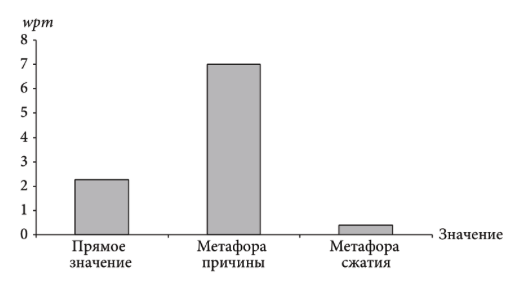
\includegraphics[width=0.8\textwidth]{img/book/pruzhina/1830-1859}
    \caption{Значения слова \textit{пружина} для 1830-1859 согласно~\cite{TwoCenturies}}
\end{figure}

\begin{figure}[H]
    \centering % Centers the images
    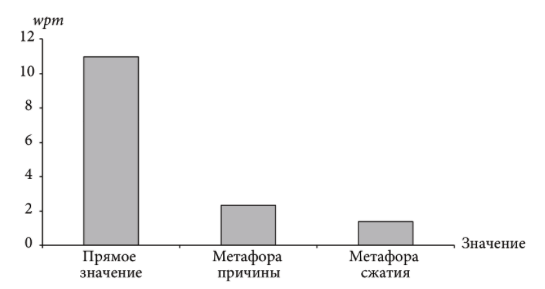
\includegraphics[width=0.8\textwidth]{img/book/pruzhina/1960-2008}
    \caption{Значения слова \textit{пружина} для 1960-2008 согласно~\cite{TwoCenturies}}
\end{figure}

Таким образом, алгоритм отражает основные значения, в которых использовалось
слово \textit{пружина}, согласуясь с данными из толкового словаря и историческим исследованием.

\section*{Публика}

В результате анализа семем лексемы \textit{публика} в толковых словарях были выделены следующие группы значений:

\begin{enumerate}
    \item Люди, присутствующие в качестве зрителей, слушателей, посетителей. \textit{Концертная, театральная публика.}
(\textit{«Лица, находящиеся где-либо в качестве посетителей, зрителей, слушателей.»} в БТС,
\textit{«Люди, находящиеся где-нибудь в качестве зрителей, слушателей, пассажиров.»} в ТСО,
\textit{«Публикой называют людей, которые собираются, присутствуют где-либо в качестве зрителей, слушателей.»} в ТСД,
\textit{«Публикой называют людей, которые собираются, присутствуют где-либо в качестве посетителей.»} в ТСД,
\textit{«Аудитория, зрители, слушатели»} в «Двух веках в двадцати словах»)

    \item Люди и общество вообще. \textit{Широкая публика.}
(\textit{«Люди, общество.»} в БТС,
\textit{«Вообще люди, общество.»} в ТСО,
\textit{«Публикой иронично называют категорию людей, которым свойственны какие-либо общие признаки.»} в ТСД)

    \item Группа лиц, объединённые по общим признакам, часто с негативной коннотацией. \textit{Знаю я эту публику - болтуны.}
(\textit{«Неодобрительно о лицах, объединённых по каким-либо признакам.»} в БТС,
\textit{«Общество или отдельные лица, объединённые по каким-н. общим признакам.»} в ТСО,
\textit{«Публикой иронично называют категорию людей, которым свойственны какие-либо общие признаки.»} в ТСД)

    \item Пассажиры, люди в общественном транспорте. \textit{Проголодавшаяся публика бросилась из вагонов в буфет.}
(\textit{«Пассажиры»} в «Двух веках в двадцати словах»,
\textit{«Люди, находящиеся где-нибудь в качестве зрителей, слушателей, пассажиров.»} в ТСО)

    \item Светское общество, привилегированный класс населения. \textit{В Москве всякий всякого по пяти раз на неделю может видеть в публике.}
(\textit{«Светское общество.»} в «Двух веках в двадцати словах»)

    \item Читатели, аудитория, воспринимающая литературные или иные творческие произведения. \textit{Теперь я понимаю, за что В*(яземский) и П*(ушкин] так любят уездных барышен. Они их истинная публика.}
(\textit{«Читатели»} в «Двух веках в двадцати словах»)

    \item Обозримая группа людей. \textit{Капитан тянул баритона, а расстрига спускал октаву, и кабацкая публика находила, что дуэты их выходят весьма чувствительны.}
(\textit{«Народец (обозримая группа людей).»} в «Двух веках в двадцати словах»)

    \item Скопление народа, уличная толпа, масса. \textit{Главные улицы, пассажи и городские ряды кишат публикой, являющейся за по-купками для обнов.}
(\textit{«Уличная толпа, масса.»} в «Двух веках в двадцати словах»)

%    \item Фразеологизмы:
%    \begin{enumerate}
%        \item Работать на публику — делать что-то с целью привлечения внимания и одобрения окружающих.
%        (\textit{«Если кто-либо работает на публику, то это означает, что этот человек делает что-либо с намерением, чтобы его действия были замечены, оценены кем-либо.»} в ТСД)
%    \end{enumerate}
\end{enumerate}

\begin{figure}[H]
	\centering
	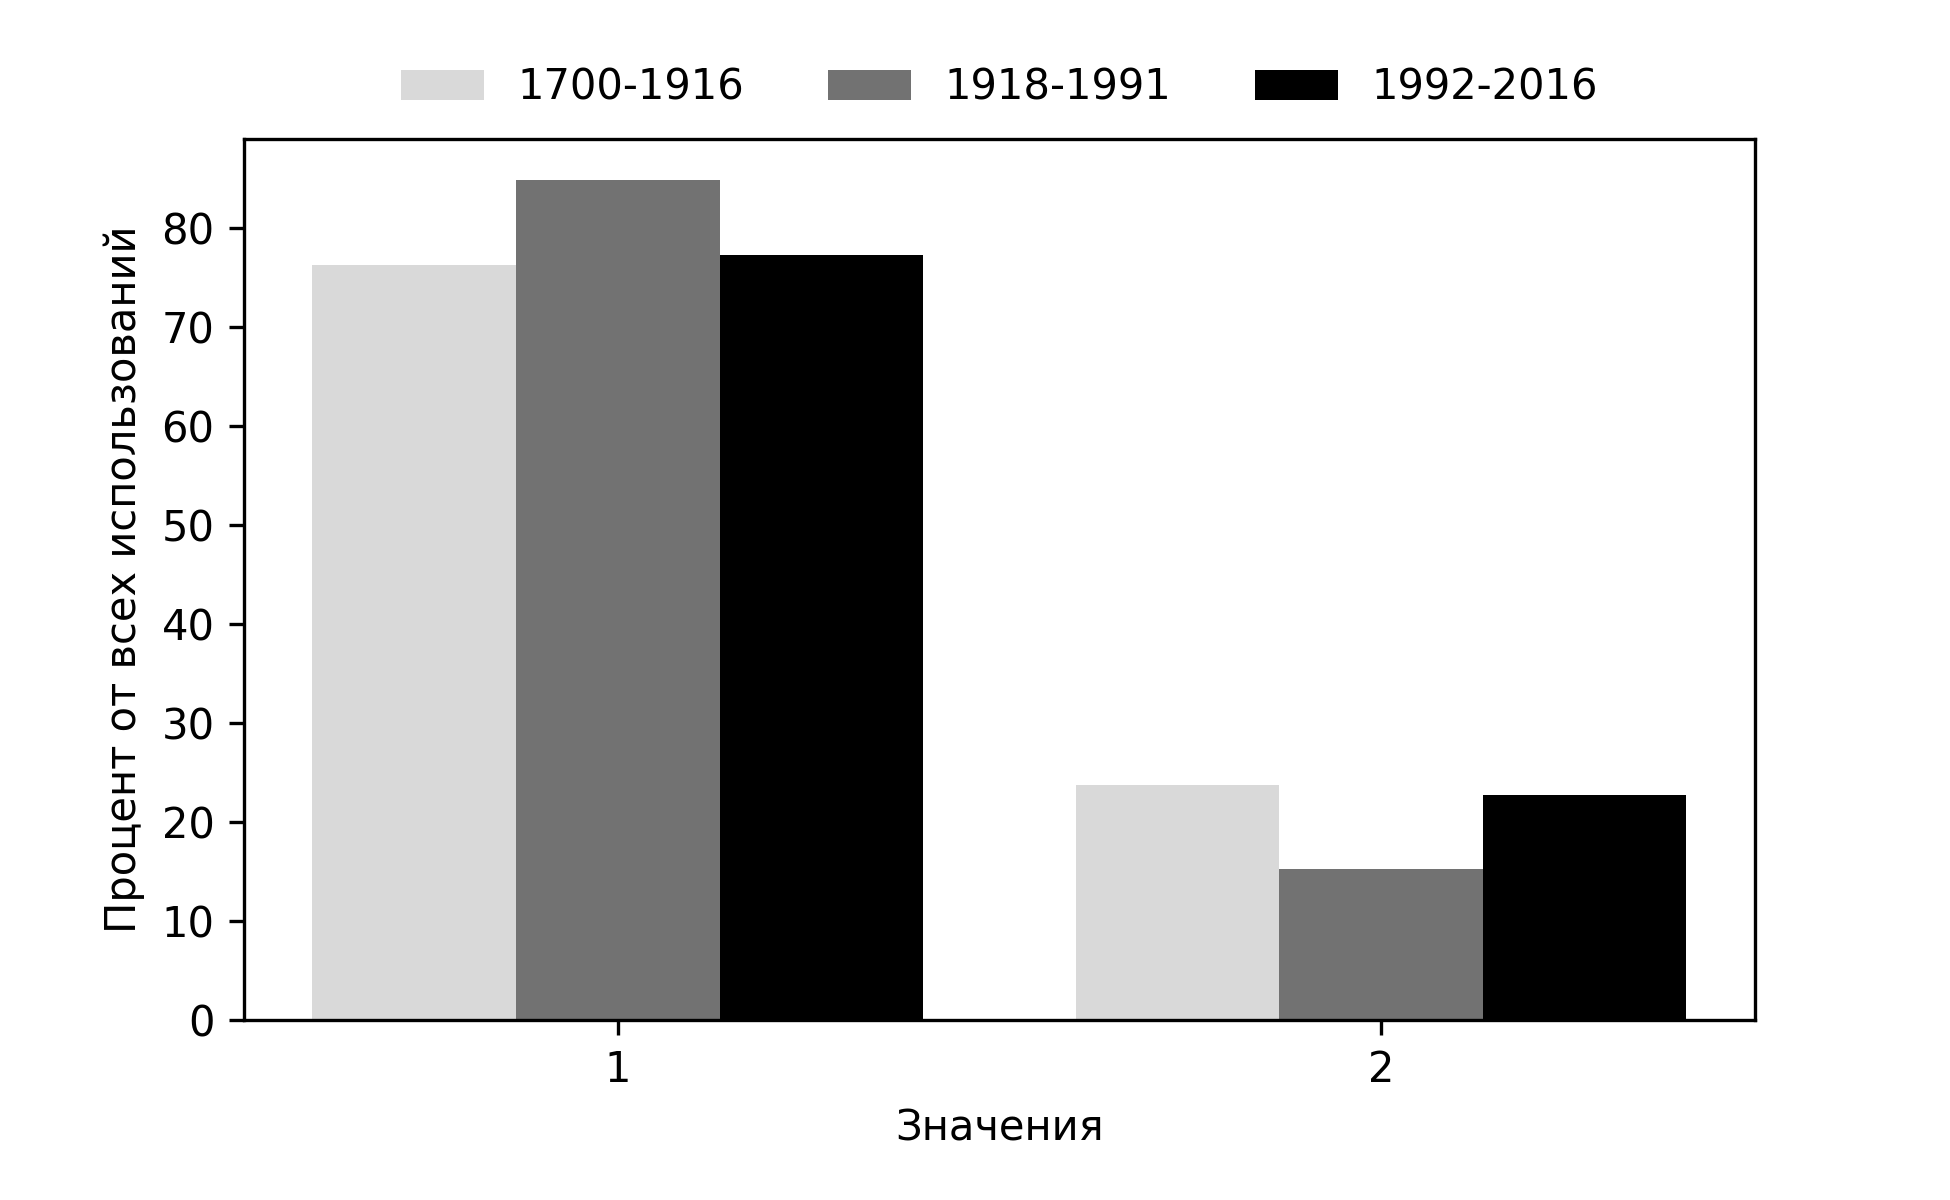
\includegraphics[width=0.8\textwidth]{img/visualizations/publika_minimal}
	\caption{Изменение значений слова \textit{Публика}}
	\label{fig:Публика}
\end{figure}

Значения для визуализации слова \textit{публика} (Параметры: eps=0.11, min\_samples=10).

\begin{enumerate}
    \item Люди, присутствующие на каком-л. собрании, спектакле, концерте и т. п.
    \item Общество, народ.
\end{enumerate}

\subsection*{Анализ значений слова \textit{публика}}

Оба определения корректно сформулированы.

Оба определения имеют явные аналоги в составленном ранее описании значений слова.

\begin{itemize}
    \item ’Люди, присутствующие на каком-л. собрании, спектакле, концерте и т. п.’ имеет соответствие с
    ’Люди, присутствующие в качестве зрителей, слушателей, посетителей.’.
    Общими смысловыми элементами являются \textit{’люди’}, \textit{’присутствующие’}, \textit{’мероприятие’}.

    \item ’Общество, народ.’ соответствует значению ’Люди и общество вообще.’.
    Общими семами являются \textit{’люди’}, \textit{’общество/народ’}.
\end{itemize}

Не предлагаются следующие значения:
\begin{itemize}
    \item ’Светское общество, привилегированный класс населения.’.
    \item ’Группа лиц, объединённые по общим признакам, часто с негативной коннотацией.’.
    \item ’Пассажиры, люди в общественном транспорте.’.
    \item ’Читатели, аудитория, воспринимающая литературные или иные творческие произведения.’.
    \item ’Обозримая группа людей.’.
    \item ’Скопление народа, уличная толпа, масса.’.
\end{itemize}

Таким образом, для лексемы \textit{публика} представлено 2 корректных определения.

Перейдем к частотности значений.

К сожалению, в книге «Два века в двадцати словах» не даётся
графиков частотности для слова \textit{публика}.
Гооврится лишь о преобладании значения ’аудитория’ и о его оттенках,
которые не удается полноценно сравнить из-за того, что алгоритм предложил довольно общие значения.

\section*{Свалка}

В результате анализа семем лексемы \textit{свалка} в толковых словарях были
выделены семь групп значений, которые можно условно сформулировать
следующим образом:

\begin{enumerate}
    \item Место для сбора мусора, нечистот. \textit{Вывезти мусор на свалку.}
(\textit{«Место, куда свозят, выбрасывают мусор, нечистоты, негодные вещи.»} в БТС,
\textit{«Место, куда вывозят, выбрасывают мусор, нечистоты, негодные вещи.»} в ТСД,
\textit{«Место для сбора мусора, нечистот»} в «Двух веках в двадцати словах»)
    \item Груда, куча, нагромождение чего-либо. \textit{Вывезти мусор на свалку.}
(\textit{«Беспорядочно накиданная груда, куча чего-л.»} и
\textit{«Если кто-либо превращает квартиру в свалку, то это означает, что там в беспорядке нагромождаются предметы, мебель и пр.»} в БТС,
\textit{«Свалкой называют беспорядочно накиданную груду каких-либо предметов.»} в ТСД,
\textit{«Груда»} в «Двух веках в двадцати словах»)
    \item Процесс сваливания. \textit{Свалка песка с платформы.}
(\textit{«к Свалить»} в БТС,
\textit{«Процесс сваливания»} в «Двух веках в двадцати словах»)
    \item Всеобщая драка. \textit{Вмешаться в свалку.}
(\textit{«Свалкой называют всеобщую драку, в которой участвует много людей»} в ТСД,
\textit{«Драка»} в «Двух веках в двадцати словах»)
    \item Скопление людей, толпа. \textit{Людская свалка.}
(\textit{«Скопление людей, толпа.»} в «Двух веках в двадцати словах» и в БТС)
    \item Вооруженное столкновение войск, битва. \textit{В жару свалки они в разных местах расстроили нашу линию, и человек 20 баварцев вдруг прорвались сквозь наш фронт.}
(\textit{«Битва»} в «Двух веках в двадцати словах»)
\end{enumerate}

\begin{figure}[H]
	\centering
	\includegraphics[width=0.8\textwidth]{img/visualizations/svalka_minimal}
	\caption{Изменение значений слова \textit{свалка} (Параметры: eps=0.12, min\_samples=25)}
	\label{fig:Свалка}
\end{figure}

Значения для визуализации слова \textit{Свалка}:

\begin{enumerate}
    \item Столкновение, драка.
    \item Беспорядочное, беспорядочное движение, толкотня.
    \item Беспорядочная, беспорядочная схватка.
    \item Место, где свалены, свалены в кучу какие-либо отходы.
    \item То, что свалено, свалено в кучу.
\end{enumerate}

Перейдем к анализу определений.

Первое определение корректно сформулированы.
Остальные определения имеют разного рода ошибки.

\begin{itemize}
    \item ’Столкновение, драка.’ соответствует ’Всеобщая драка.’, так как
имеет общий смысловой элемент, а именно семы \textit{’столкновение’} и \textit{’драка’}.

    \item ’Место, где свалены, свалены в кучу какие-либо отходы.’ соответствует
’Место, куда свозят, выбрасывают мусор, нечистоты, негодные вещи.’,
так как включает те же семы \textit{’место’}, \textit{’свалены’}, \textit{’отходы’}.
Однако повторение слова \textit{свалены} является ошибкой в генерации.
\end{itemize}

\begin{itemize}
    \item ’Беспорядочное, беспорядочное движение, толкотня.’ частично соответствует
’Скопление людей, толпа.’, которое также указано в «Двух веках в двадцати словах» как ’Толпа, давка.’,
так как подразумевает собрание большого количества людей.
Однако повторение слова \textit{беспорядочное} является ошибкой в генерации,
что также относит определение к избыточным.

    \item ’Беспорядочная, беспорядочная схватка.’ соответствует
’Всеобщая драка.’, включает семы \textit{’потасовка’}, \textit{’с участием большого количества людей’}.
Повторение слова \textit{беспорядочная} является ошибкой в генерации,
соответственно данное определение будет определено как избыточное.

    \item ’То, что свалено, свалено в кучу.’ соответствует
‘Груда, куча, нагромождение чего-либо.’, так как оба определения акцентируют внимание
на неорганизованном скоплении чего-либо.
Повторение слова \textit{свалено} является ошибкой в генерации,
поэтому мы классифицируем это определение как имеющее избыточность.
\end{itemize}

Обобщённые значения, не найденные в визуализации:

\begin{itemize}
    \item ’Процесс сваливания’ также отсутствует в визуализации.
%Это значение указывает на процесс, а не на результат, что могло быть причиной его отсутствия в предсказаниях модели.
Согласно~\cite{TwoCenturies}, это значение не является частым, что могло быть причиной отсутствия в визуализации.

    \item ’Вооруженное столкновение войск, битва’ отсутствует среди предложенных моделью значений.
Это значение не является частым, что могло быть причиной его невключения в результат.
\end{itemize}

Определения, предложенные алгоритмом с повторением слов, далее будут написаны без повторения.

Таким образом, для лексемы \textit{свалка} представлено 1 корректное определение.
Среди ошибок присутствует:
\begin{itemize}
    \item Избыточность или чрезмерное использование общих фраз: 3
    \item Близкое значение, а также избыточность или чрезмерное использование общих фраз: 1
\end{itemize}

Перейдем к частотности значений.

В книге «Два века в двадцати значениях» как появившееся в 1900-ых годах указано
значение \textit{«Место для сбора мусора, помойка.»}, соответствующее четвёртому значению,
предложенному алгоритмом ’Место, где свалены, в кучу какие-либо отходы.’.
Как видно из графика результатов алгоритма, оно почти не используется в досоветский период,
но становится главным
с 60\% использования в советский период и доминирует в постсоветский с около 85\%.
Эти данные совпадают с тем, что говорится в книге, где утверждается 87\% использования
значения \textit{«Помойка.»} в 1998-1997 годы, 32\% для 1925-1949 годов.

Уменьшается же судя по графику преимущественно значение 1 (’Столкновение, драка.’),
которое падает с 50\% использований в досоветский период до 5\% в постсоветский.
В книге резульаты схожи.
Так, утверждается, что в 1875-1899 году слово имело значение ’Драка.’
в 71\% использований,
а к 1998-1997 значение упало до 12\%.

\noindent % Prevents indentation for this line to align the images at the left margin
\begin{figure}[H]
    \centering % Centers the images
    \includegraphics[width=0.32\textwidth]{img/book/Свалка 1998-1999}
    \hfill % Fills the space between the images
    \includegraphics[width=0.32\textwidth]{img/book/Свалка 1875-1799}
    \hfill % Fills the space between the images
    \includegraphics[width=0.32\textwidth]{img/book/Свалка 1925-1949}
    \caption{Визуализации для слова \textit{свалка} согласно~\cite{TwoCenturies}}
\end{figure}

Таким образом, модель довольно точно отражает реальное изменение значений слова \textit{свалка}
во времени, согласуясь с данными из толкового словаря и историческим исследованием.
Она адекватно выделяет как наиболее широко используемое сегодня значение,
связанное с местом сбора мусора,
так и менее очевидные значения, включая драку,
однако предложенные моделью определения имеют излишние повторения слов.

\section*{Сволочь}

В результате анализа семем лексемы \textit{сволочь} в толковых словарях были выделены шесть групп значений,
которые можно условно сформулировать следующим образом:

\begin{enumerate}
    \item Подлый, скверный человек; негодяй. \textit{Обманул-таки, сволочь.!}
(\textit{«Грубо. Скверный, подлый человек; негодяй.»} в БТС,
\textit{«Негодяй, мерзавец.»} в ТСО,
\textit{«Подлец»} в «Двух веках в двадцати словах»)

    \item Собирательное наименование для дрянных, подлых людей; сброд, подонки. \textit{Всякая сволочь.}
(\textit{«собир. Дрянные, подлые люди; сброд, подонки.»} в БТС,
\textit{«собир. Сброд, подлые люди.»} в ТСО,
\textit{«Сброд»} в «Двух веках в двадцати словах»)

    \item Военный сброд, разброд войска. \textit{Многочисленные колонны наши обратились в буйную сволочь, в которой солдаты разных полков были чужды один другому}
(\textit{«Вольница, военный сброд»} в «Двух веках в двадцати словах»)

    \item Малые люди, чернь, мелкая канцелярская чернь. \textit{...на другой день вся эта мелкая канцелярская сволочь явилась у меня в передней с поклонами, поздравлениями и доносами.}
(\textit{«Маленькие люди, чернь»} в «Двух веках в двадцати словах»)

    \item Сборище, компания. \textit{Вчера я обедал со всею сволочью здешних литераторов.}
(\textit{«Сборище»} в «Двух веках в двадцати словах»)

    \item Экспрессивное восклицание, выражающее негативные эмоции. \textit{Крепкое, сволочь! Аж в голову ступило...}
(\textit{«Экспрессивное восклицание»} в «Двух веках в двадцати словах»)
\end{enumerate}

\begin{figure}[H]
	\centering
	\includegraphics[width=0.8\textwidth]{img/visualizations/svoloch'_minimal}
	\caption{Изменение значений слова \textit{cволочь}}
	\label{fig:Сволочь}
\end{figure}

Значения для визуализации слова \textit{cволочь} (Параметры: eps=0.1, min\_samples=10).

\begin{enumerate}
    \item Употребляется как бранное слово.
%    \item Таща, доставить куда-либо.
    \item О подлом, гнусном человеке.
\end{enumerate}

\subsection*{Анализ значений слова \textit{сволочь}}

Определения корректно сформулированы.

\begin{itemize}
    \item ’Употребляется как бранное слово.’ имеет общий смысловой элемент с
’Экспрессивное восклицание, выражающее негативные эмоции.’,
а именно семы \textit{’бранное слово’} и \textit{’экспрессивное восклицание’}.

    \item ’О подлом, гнусном человеке.’ соответствует
    ’Подлый, скверный человек; негодяй.’, так как включает те же семы \textit{’подлый’}, \textit{’гнусный’}.
\end{itemize}

%\begin{itemize}
%    \item ’Таща, доставить куда-либо.’ является некорректным значением,
%    так как в обобщенных значениях нет упоминания о действии «тащить» или «доставлять».
%\end{itemize}

Обобщённые значения, не найденные в визуализации:
\begin{itemize}
    \item ’Собирательное наименование для дрянных, подлых людей; сброд, подонки’ отсутствует среди предложенных моделью значений.
%Возможно, информации из контекста использований недостаточно для выявления этого значения.

    \item ’Военный сброд, разброд войска’ также отсутствует в визуализации.
Это может быть связано с редкостью использования данного значения в контекстах датасета.

    \item ’Малые люди, чернь, мелкая канцелярская чернь’ также не представлено в визуализации,
что может указывать на недостаточное количество примеров с этим значением в датасете.

    \item ’Сборище, компания’ также не было явно выделено.
\end{itemize}

Таким образом, для лексемы \textit{сволочь} представлено 2 корректных определения.

Перейдем к частотности значений.

К сожалению, оба выделенных значения подпадают под значение ’Индивидуальное оскорбление.’
в книге «Два века в двадцати словах».
Также в визуализации отсутствуют ключевые значения,
которые часто использовались в досоветский период, такие как ’Собирательное наименование для дрянных, подлых людей; сброд, подонки’.
Таким образом, анализ изменений значения сделать не представляется возможным.

\section*{Стиль}

В результате анализа семем лексемы \textit{стиль} в толковых словарях были выделены следующие группы значений,
которые можно условно сформулировать следующим образом:

\begin{enumerate}
    \item Совокупность признаков, черт, приёмов, создающих целостный образ искусства определённого времени, направления, индивидуальной манеры художника. \textit{Стили в живописи.}
(\textit{«Совокупность признаков, черт, создающих целостный образ искусства определённого времени, направления, индивидуальной манеры художника в отношении идейного содержания и художественной формы.»} в БТС,
\textit{«Совокупность черт, близость выразительных художественных приёмов и средств, обусловливающие собой единство какого-н. направления в творчестве.»} в ТСО,
\textit{«Стилем называют жанровую и тематическую направленность художественного произведения.»} и \textit{«Стилем называют совокупность литературных приёмов, характерных для какого-либо направления, жанра, произведения.»} в ТСД,
\textit{«Особенности направления архитектуры»} в «Двух веках в двадцати словах»)

    \item Способ летоисчисления. \textit{Новый стиль.}
(\textit{«Способ летосчисления.»} в БТС, ТСО и ТСД,
\textit{«Способ летоисчисления»} в «Двух веках в двадцати словах»)

    \item Способ, метод, совокупность приёмов осуществления какой-либо деятельности, работы. \textit{Стиль руководства.}
(\textit{«Способ осуществления чего-л., характер деятельности, работы в их отличительных признаках.»} в БТС,
\textit{«Метод, совокупность приёмов какой-н. работы, деятельности, поведения.»} в ТСО,
\textit{«Стилем называется способ осуществления чего-либо.»} в ТСД)

    \item Совокупность приёмов использования языковых средств. \textit{Романтический стиль.}
(\textit{«Совокупность приёмов использования средств языка, характерная для какого-л. писателя или литературного произведения, направления, жанра.»} в БТС,
\textit{«Совокупность приёмов использования языковых средств для выражения тех или иных идей, мыслей в различных условиях речевой практики, слог.»} и \textit{«Совокупность приёмов использования языковых средств, а также вообще средства художественной выразительности, определяющие своеобразие творчества писателя, отдельного произведения.»} в ТСО,
\textit{«Характеристика языковых средств»} в «Двух веках в двадцати словах»)

    \item Индивидуальная манера художника, писателя. \textit{Свой стиль Щедрин называет эзоповским.}
(\textit{«Стилем называют индивидуальную авторскую манеру, которая ощущается читателем, зрителем в нескольких произведениях одного автора.»} в ТСД,
\textit{«Черты, свойственные конкретному человеку (например, деятелю искусства)»} в «Двух веках в двадцати словах»)

    \item Совокупность наиболее характерных черт в искусстве какого-либо народа, страны, региона. \textit{Русский стиль.}
(\textit{«совокупность наиболее общих черт в искусстве какого-л. народа, страны, региона, отличающихся от искусства соседних народов и т.п..»} в БТС,
\textit{«Стилем называют совокупность наиболее характерных черт в искусстве какого-либо народа, страны и т. п.»} в ТСД)

    \item Манера словесного изложения. \textit{Лаконичный стиль.}
(\textit{«Построение речи в соответствии с нормами литературного языка, манера словесного изложения.»} в БТС,
\textit{«Стилем называют чью-либо манеру словесного изложения какой-либо информации.»} в ТСД)

    \item Функциональная разновидность литературного языка. \textit{Официально-деловой стиль.}
(\textit{«Функциональная разновидность литературного языка.»} в БТС,
\textit{«Стилем называют функциональную разновидность литературного языка.»} в ТСД)

    \item Характерная манера совершения движения, в т.ч. в спорте. \textit{Стили гребли.}
(\textit{«Совокупность признаков, черт, приёмов, выделяющих какую-л. вещь, предмет на фоне аналогичных и образующих их суть (в спорте).»} в БТС,
\textit{«Стилем называют характерную манеру совершения движения.»} в ТСД)

    \item Модное веяние в одежде, совокупность признаков, черт вещей, одежды. \textit{Джинсовый стиль.}
(\textit{«Совокупность признаков, черт, отличающих направление, вещь от других (в моде, в одежде).»} в БТС,
\textit{«Стилем называют модное веяние, которое воспринято многими.»} в ТСД)

    \item Изменяющаяся социальная форма жизни, деятельности. \textit{Московский стиль жизни.}
(\textit{«Совокупность признаков общественной жизни, активности в тот или иной период.»} в БТС,
\textit{«Стилем называют изменяющуюся социальную форму жизни, деятельности.»} в ТСД)

    \item Индивидуальная манера поведения, общения, одежды и т.п. \textit{Стиль поведения, общения.}
(\textit{«Индивидуальная манера осуществления какой-л. деятельности, работы, проявления личных качеств в разговоре, поведении, одежде и т.п.»} в БТС,
\textit{«Стилем называют изменяющуюся индивидуальную форму жизни, деятельности.»} и \textit{«Манера, совокупность особенностей по отношению к широкому кругу явлений (поведение, одежда, взгляды, внешность, интерьер)»} в «Двух веках в двадцати словах»)

%    \item В стиле кого-либо, чего-либо (следование примеру, подражание кому-либо, чему-либо).
%(\textit{«Если кто-либо делает что-либо в стиле кого-либо, чего-либо, то это означает, что этот человек следует примеру кого-либо, подражает чему-либо и т. п.»} в ТСД)

\end{enumerate}

\begin{figure}[H]
	\centering
	\includegraphics[width=0.8\textwidth]{img/visualizations/stil'_minimal}
	\caption{Изменение значений слова \textit{стиль}}
	\label{fig:Стиль_книга}
\end{figure}

Значения для визуализации слова \texit{стиль} (Параметры: eps=0.15, min\_samples=25).

\begin{enumerate}
    \item Совокупность художественных приемов, характерных для какого-либо искусства, литературы и т. п.
    \item Система летосчисления, принятая в какой-л. стране, а также время по этой системе.
    \item Характер, манера, образ действий, поведения кого-либо.
\end{enumerate}

Перейдем к анализу определений.

Определения корректно сформулированы.

\begin{itemize}
    \item ’Совокупность художественных приемов, характерных для какого-либо искусства, литературы и т. п.’ имеет общий смысловой элемент с
’Совокупность признаков, черт, приёмов, создающих целостный образ искусства определённого времени, направления, индивидуальной манеры художника.’,
%’Индивидуальная манера художника, писателя.’
’Совокупность наиболее характерных черт в искусстве какого-либо народа, страны, региона.’, а также
’Совокупность приёмов использования языковых средств.’,
а именно компоненты значения \textit{’совокупность’}, \textit{’приемы’}, \textit{’искусство’}, \textit{’литература’}.

    \item ’Система летосчисления, принятая в какой-л. стране, а также время по этой системе’ полностью соответствует
’Способ летоисчисления.’, так как включает те же семы \textit{’система’}, \textit{’летосчисление’}, \textit{’страна’}.
\end{itemize}

\begin{itemize}
    \item ’Характер, манера поведения кого-либо.’ наиболее близко к
’Индивидуальная манера поведения, общения, одежды и т.п.’
\end{itemize}

Обобщённые значения, не найденные в визуализации:
\begin{itemize}
    \item ’Функциональная разновидность литературного языка.’ отсутствует среди предложенных моделью значений.
Можно предположить, что информации из контекста использований недостаточно для отделения этого значения от ’Совокупность художественных приемов, характерных для какого-либо искусства, литературы и т. п.’.

    \item ’Модное веяние в одежде, совокупность признаков, черт вещей, одежды.’ также отсутствует в визуализации.
%Однако, модель способна на выделение данного значения.

    \item ’Изменяющаяся социальная форма жизни, деятельности.’ и ’Характерная манера совершения движения, в т.ч. в спорте.’ также отсутствуют.
Возможно, эти значения не были включены из-за их меньшей частоты в исследуемом материале.
\end{itemize}

Таким образом, для лексемы \textit{стиль} представлены 3 корректные определения.

Перейдем к частотности значений.

К сожалению, в книге «Два века в двадцати словах» указано,
что все значения слова «стиль» появились в досоветский период,
а также все графики даны только для этого периода.
Однако в книге говорится, что частота употребления значения ’Способ летоисчисления.’
снижается значительно с досоветского периода, что согласуется с данными нашего исследования.
В остальном, представляется затруднительным сравнение результатов модели с данными из книги.

\begin{figure}[H]
    \centering % Centers the images
    \includegraphics[width=0.8\textwidth]{img/book/stil'/1860-1899}
    \caption{Визуализации для слова \textit{стиль} для 1860-1899 согласно~\cite{TwoCenturies}}
    \label{fig:Стиль}
\end{figure}

\section*{Тётка}

В результате анализа семем лексемы \textit{тётка} в толковых словарях были выделены следующие группы значений:

\begin{enumerate}
    \item Вообще женщина. \textit{Уселись тётки на лавочке.}
(\textit{«Обо всякой взрослой женщине.»} в БТС,
\textit{«Тёткой грубо называют женщину или девушку.»} в ТСД,
\textit{«Вообще женщина (чаще пожилая).»} в ТСО,
\textit{«Женщина (вне контекста обращения)»} в «Двух веках в двадцати словах»)

    \item Сестра отца или матери, а также жена дяди.  \textit{Родная, двоюродная тётка.}
(\textit{«Сестра отца или матери, а также жена дяди.»} в ТСО,
\textit{«Тёткой называют сестру матери или отца.»} в ТСД,
\textit{«=Тётя (1 зн.).»} в БТС,
\textit{«Сестра матери.»} в «Двух веках в двадцати словах»)

    \item Обращение к незнакомой женщине. \textit{— Не хлопочи, тётка, — сказал Алексей, войдя в избу.}
(\textit{«Обращение к незнакомой женщине (ед. или мн. ч.)»} в «Двух веках в двадцати словах»)

    \item Незнатная женщина, употребляется вместе с именем.
(\textit{«Называние незнатной женщины в форме «тётка + имя»»} в «Двух веках в двадцати словах»)
%    \item Фразеологизм «Голод не тётка».
%    (\textit{«Голод не тётка (Погов.)»} в БТС,
%    \textit{«Голод не т. (посл. о проголодавшемся; шутл.)»} в ТСО,
%    \textit{«Фраза Голод не тётка употребляется в том случае, если речь идёт о чьём-либо нестерпимом желании поесть, утолить голод.»} в ТСД)
%
    \item Карточная игра. \textit{Играют в «тётку».}
(\textit{«Карточная игра»} в «Двух веках в двадцати словах»)
\end{enumerate}

\begin{figure}[H]
	\centering
	\includegraphics[width=0.8\textwidth]{img/visualizations/tetka_minimal}
	\caption{Изменение значений слова \textit{тётка}}
	\label{fig:Тётка}
\end{figure}

Значения для визуализации слова \textit{тётка} (Параметры: eps=0.1, min\_samples=15).

\begin{enumerate}
    \item Родная сестра отца или матери.
    \item Женщина средних лет.
\end{enumerate}

\subsection*{Анализ значений слова \textit{тётка}}

Первое определение корректно сформулировано.
Второе определение имеет слишком узкое значение, так как в словарях значение охватывает всех взрослых женщин,
а не только женщин средних лет.

\begin{itemize}
    \item ’Родная сестра отца или матери.’ имеет общий смысловой элемент с
’Сестра отца или матери, а также жена дяди.’, а именно семы \textit{’родственник’}, \textit{’сестра одного из родителей’}.

    \item ’Женщина средних лет.’ соответствует ’Вообще женщина.’, хоть и более узкое,
так как обобщенное определения включает всех женщин, а не только женщин средних лет.
Сема \textit{’средних лет’} делает его слишком узким.
\end{itemize}

Обобщённые значения, не найденные в визуализации:
\begin{itemize}
    \item ’Обращение к незнакомой женщине.’, как и ’Незнатная женщина.’ моделью отдельно от
’Женщина средних лет.’ не выделяется.

    \item ’Карточная игра’ также отсутствует в визуализации.
Его отсутствие обусловлено тем, что это значение не так часто встречается в исследуемом корпусе.
Данное определение указано только в «Двух веках в двадцати словах», где приводятся только
единичные использования слова в этом значении, не влияющие в целом на статистику значений.
\end{itemize}

Таким образом, для лексемы \textit{тётка} представлено 1 корректное определение.
Среди ошибок присутствует:
\begin{itemize}
    \item Избыточно конкретизированные: 1
\end{itemize}

Перейдем к частотности значений.

Главным изменением для слова \textit{тётка} является появление в конце советского периода
его использования по отношению ко всем женщинам, а не только родственницам (30\% для 1980-1985 гг.
и около 5\% для 1910-1920 и 1940-1954 гг.), что приводится в графиках снизу.
К сожалению, в книге не приводится информация об использовании слова в постсоветский период.
Данные из нашей визуализации согласуются с вышеописанными изменениями.
Так, значение ’Женщина средних лет.’ появляется в советский период с около 10\%
использований и выходит на лидирующие позиции в постсоветский период с больше 60\%.

\noindent % Prevents indentation for this line to align the images at the left margin
\begin{figure}[H]
    \centering % Centers the images
    \includegraphics[width=0.8\textwidth]{img/book/tetka/1800-1899}
    \caption{Значения слова \textit{тётка} для 1800-1899 согласно~\cite{TwoCenturies}}
\end{figure}

\begin{figure}[H]
    \centering % Centers the images
    \includegraphics[width=0.8\textwidth]{img/book/tetka/1910-1985}
    \caption{Значения слова \textit{тётка} для 1910-1985 согласно~\cite{TwoCenturies}}
\end{figure}

Таким образом, алгоритм полностью отражает значения, в которых использовалось
слово \textit{тётка}, согласуясь с данными из толкового словаря и историческим исследованием.

\section*{Червяк}

В результате анализа семем лексемы \textit{червяк} в толковых словарях были выделены четыре группы значений,
которые можно условно сформулировать следующим образом:

\begin{enumerate}
    \item Маленькое беспозвоночное животное. \textit{Дождевой червяк.}
    (\textit{«=Червь (1.Ч.; 1-2 зн.).»} в БТС,
    \textit{«То же, что червь.»} в ТСО,
    \textit{«Маленькое беспозвоночное животное»} в «Двух веках в двадцати словах»)

    \item Ничтожное, жалкое создание. \textit{Я ваш червяк.}
    (\textit{«О жалком, ничтожном человеке (презр)»} в ТСО,
    \textit{«Ничтожное создание»} в «Двух веках в двадцати словах»)

    \item Тревожное, мучительное чувство. \textit{Червяк гложет сердце.}
    (\textit{«О постоянном наличии какого-л. чувства, состояния, плохо воздействующего на кого-л.»} в БТС,
\textit{«Внутренний паразит»} в «Двух веках в двадцати словах»)

    \item Техническое приспособление в виде винта для передачи движения. \textit{Червяк износился.}
    (\textit{«Проф. Червячная передача; деталь механизма для такой передачи.»} в БТС,
    \textit{«Зубчатое колесо в форме винта для передачи движения в нек-рых механизмах (спец.)»} в ТСО,
    \textit{«Техническое приспособление»} в «Двух веках в двадцати словах»)
\end{enumerate}

\begin{figure}[H]
	\centering
	\includegraphics[width=0.7\textwidth]{img/visualizations/chervjak_minimal}
	\caption{Изменение значений слова \textit{червяк}}
	\label{fig:Червяк}
\end{figure}

Значения для визуализации слова \textit{червяк} (Параметры: eps=0.16, min\_samples=10).

\begin{enumerate}
    \item Насекомое, похожее на червя, а также его личинка.
    \item О мелком, ничтожном человеке.
    \item Употребляется как бранное слово.
    \item О ком-, чем-либо маленьком, тонком, извивающемся.
    \item О каком-л. неприятном, мучительном чувстве, испытываемом кем-л.
\end{enumerate}

\subsection*{Анализ значений слова \textit{червяк}}

Второе и пятое определения корректно сформулированы.
Первое, третье и четвертое определения не соответствуют обобщенным значениям.

\begin{itemize}
    \item ’Насекомое, похожее на червя, а также его личинка.’ имеет общий смысловой элемент с
’Маленькое беспозвоночное животное.’, а именно семы \textit{’маленькое’}, \textit{’животное’}, \textit{’беспозвоночное’}.
Тем не менее, оно содержит ошибку, а именно то, что червь не является насекомым.

    \item ’О мелком, ничтожном человеке.’ соответствует
’Ничтожное, жалкое создание.’, так как включает те же семы \textit{’ничтожность’}, \textit{’жалкость’}.

    \item ’О каком-л. неприятном, мучительном чувстве, испытываемом кем-л.’ соответствует
’Тревожное, мучительное чувство.’, так как включает семы \textit{’неприятное’}, \textit{’мучительное’} и
\text{’чувство’}.
\end{itemize}

\begin{itemize}
    \item ’Употребляется как бранное слово.’ является близким значением к
’Ничтожное, жалкое создание.’, так как бранное слово может указывать на презрение,
но не полностью соответствует исходному значению.

    \item ’О ком-, чем-либо маленьком, тонком, извивающемся.’ является близким значением к
’Маленькое беспозвоночное животное.’, которое не раскрывает отличительные стороны денотата.
\end{itemize}

Обобщённые значения, не найденные в визуализации:
\begin{itemize}
    \item ’Техническое приспособление в виде винта для передачи движения.’ отсутствует среди
предложенных моделью значений.
Модель способна на выделение этого значения, сгенерировав
’металлический стержень, служащий для передачи вращательного движения’ для вхождения
\textit{При установке киноаппарата в боксе надо следить за тем, чтобы червячное колесо и
червяк вошли в зацепление.}
Вероятно, модель не распознала это значение из-за его редкости в общем корпусе текстов.
\end{itemize}

Таким образом, для лексемы \textit{червяк} представлены 2 корректных определения.
Среди ошибок присутствуют:
\begin{itemize}
    \item Близкие значения: 3
\end{itemize}

Перейдем к частотности значений.

В книге «Два века в двадцати словах» не даётся графиков изменения частоты использования значений
для слова \textit{червяк}, однако упоминается о том, что значения
’Ничтожное, жалкое создание.’ и ’Тревожное, мучительное чувство.’
реже используются со временем, особенно во второй половине XX века.
Эти данные подтверждаются в нашей визуализации, где использование
’О мелком, ничтожном человеке.’ падает с 20\% в досоветский период до 10\% в советский и постсоветский,
а также использование ’О каком-л. неприятном, мучительном чувстве, испытываемом кем-л.’
уменьшается с около 8\% в досоветский период до 1-2\% в советский и 3\% в постсоветский.

Таким образом, алгоритм в целом отражает значения, в которых использовалось
слово \textit{червяк}, согласуясь историческим исследованием, но допуская различного рода ошибки
в 3 из 5 сгенерированных определениях.

\chapter{Обучение модели}

\begin{longtable}{ll}
\caption{LoRa параметры} \\
\hline
\textbf{Параметр} & \textbf{Значение} \\
\hline
r & 32 \\
lora\_alpha & 64 \\
lora\_dropout & 0.1 \\
\hline
\end{longtable}

\begin{longtable}{ll}
\caption{Trainer параметры} \\
\hline
\textbf{Параметр} & \textbf{Значение} \\
\hline
learning\_rate & 1e-3 \\
lr\_scheduler\_type & linear \\
batch\_size & 16 \\
gradient\_checkpointing & true \\
gradient\_accumulation\_steps & 1 \\
weight\_decay & 0.1 \\
optimizer & adafactor \\
num\_train\_epochs & 6 \\
\hline
\end{longtable}

\chapter{Дообучение векторизатора}

\begin{table}[H]
\centering
\begin{tabular}{|l|l|}
\hline
\textbf{Hyperparameter}    & \textbf{Value} \\ \hline
Batch size                 & 32    \\ \hline
Loss function              & CosineSimilarityLoss \\ \hline
Epochs                     & 2     \\ \hline
Warmup steps               & 100   \\ \hline
Evaluation steps           & 50    \\ \hline
Training data split ratio  & 80/20 \\ \hline
Random seed                & 42    \\ \hline
\end{tabular}
\caption{Параметры дообучения векторизатора}
\label{tab:hyperparameters}
\end{table}


\end{document}
